%!TEX root = ../../PhD_thesis__Edouard_Leurent.tex

\graphicspath{{2-Chapters/7-Chapter/}}

\chapter{Preparing for the Worst}
\label{chapter:7}

\begin{flushright}
	\begin{tabular}{@{}l@{}}
		\emph{Two roads diverged in a wood, and I--}\\
		\emph{I took the one less traveled by,}\\
		\emph{And that has made all the difference.}\\
	\end{tabular}
	
%	Robert Frost, \href{https://eleurent.github.io/sisyphe/texts/the-road-not-taken.html}{\enquote{The Road Not Taken}}. \emph{Mountain Interval}.
	Robert Frost, \href{https://eleurent.github.io/sisyphe/texts/the-road-not-taken.html}{\emph{The Road Not Taken}}.
\end{flushright}

\abstractStartChapter{}%
Model-based algorithms often assume a \emph{certainty equivalence} to decouple estimation and control: they use a point estimate $\hat{\Ps}$ of the dynamics as if it was the true value. Unfortunately, this \textit{model bias} can significantly degrade the performances. In this chapter, we address this issue by resorting to \emph{robust} decision-making: instead of a mere point estimate, we build a \emph{confidence region} that contains the true dynamics $\Ps$ with high probability, and consider the worst-case outcome with respect to this uncertainty. We propose an integrated framework leveraging non-asymptotic linear regression, interval prediction and tree-based planning to achieve robust stabilisation and minimax control with generic costs; along with an end-to-end analysis.\footnote{This chapter is based on two articles published in the \emph{2019 and 2020 Conferences on Decision and Control} \citep{Leurent2019interval,Leurent2020robust} and one submitted to the \emph{2020 Conference on Neural Information Processing Systems} \citep{Leurent2020beyond}.}
\minitocStartChapter{}

\section{Motivation}
\label{sec:robust-motivation}

\begin{remark}[Change of notations]
\begin{leftbar}[remarkbar]
So far, we borrowed notations from the \glsxtrlong*{RL} community to describe states $s\in \cS$, actions $a\in\cA$ and transitions $s_{t+1} = \Ps\parentheses{s_{t+1}\mid s_t,a_t}$. In this chapter, we change conventions and switch to notations from the Control community, which are better suited to describe continuous-time dynamics: states are denoted as $x(t)$, controls as $u(t)$, and dynamics as $\dot{x}(t) = f(x(t), u(t))$. 
The system dynamics are described in continuous time, but sensing and control are performed in discrete time with time-step $\timestep>0$. For any variable $z$, we use subscript to refer to these discrete times: $z_n = z(t_n)$ with $t_n = n\timestep$ and $n\in\Natural$. We use bold symbols to denote temporal sequences $\bz = (z_n)_{n\in\Natural}$.
\end{leftbar}
\end{remark}

% --- 1. Model bias and robust control
\paragraph{Model bias}
Despite the recent successes of Reinforcement Learning \citep[\eg][]{Mnih2015humanlevel,Silver2018}, it has hardly been applied in real industrial issues. This could be attributed to two undesirable properties which limit its practical applications. First, it depends on a tremendous amount of interaction data that cannot always be simulated. This issue can be alleviated by model-based methods -- which we consider in this part -- that often benefit from better sample efficiencies than their model-free counterparts. Second, it relies on trial-and-error and random exploration, which is unacceptable in a critical setting where mistakes are costly and must be avoided at all time.

Since experiencing failures is out of the question, the only way to prevent them from the outset is to rely on some sort of prior knowledge. In this chapter, we assume that the system dynamics are \emph{partially known}, in the form of differential equation with unknown parameters and inputs. More precisely,

\begin{assumption}[Structure \textsc{I}]
\begin{leftbar}[assumptionbar]
We consider a dynamical system with state $x\in\Real^p$, acted on by controls $u\in\Real^q$ and perturbations $\omega\in\Real^r$, with dynamics in the form
\begin{equation*}
\dot{x}(t) = f_\theta\left(x(t),u(t),\omega(t)\right),
\end{equation*}
where the dynamics structure $f:\theta\rightarrow f_\theta$ is \emph{known}, and the parameter vector $\gls+{params}$ belongs to a known compact set $\Theta \subset \Real^d$.
\end{leftbar}
\end{assumption}
\noindent We argue that this structure assumption is realistic given that most industrial applications to date have been relying on physical models to describe their processes and well-engineered controllers to operate them, rather than machine learning. Our framework relaxes this modelling effort by allowing some \emph{structured uncertainty} around the nominal model.

We adopt a data-driven scheme to estimate the parameters $\theta$ more accurately as we interact with the true system. Most model-based reinforcement learning algorithms rely on the estimated dynamics $\hat{\theta}$ to derive the corresponding optimal controls \citep[\eg][]{Lenz2015,Levine2016}, but suffer from \emph{model bias}: they ignore the error between the learned and true dynamics, which can dramatically degrade control performances \citep{Doyle1978,Schneider1997}. 


\begin{figure}[ht]
	\begin{center}
		\begin{subfigure}[t]{0.45\linewidth}
			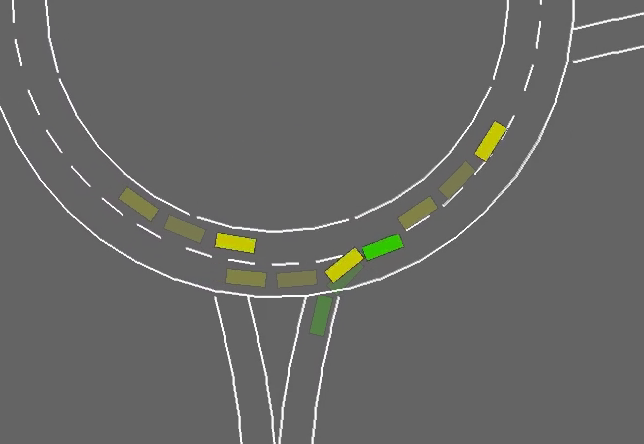
\includegraphics[width=\linewidth]{img/bias-oracle}
			\caption{Optimal control (\gls{RL}) operates near constraint saturation which produces risky behaviours.}
			\label{fig:bias-oracle}
		\end{subfigure}\hfill
		\begin{subfigure}[t]{0.46\linewidth}
			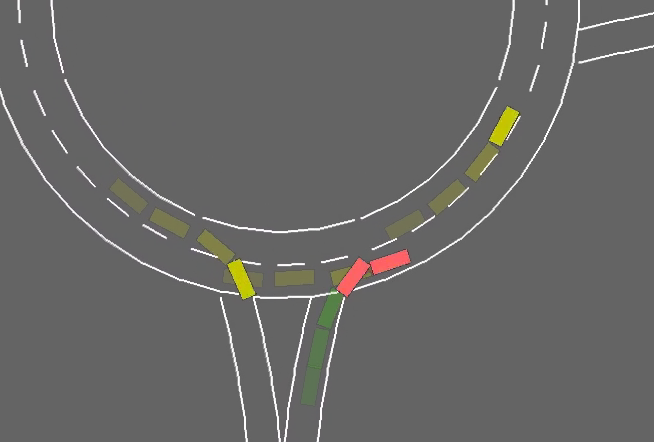
\includegraphics[width=\linewidth]{img/bias-bias}
			\caption{As a result, model bias easily causes accidents when predictions are slightly wrong (here by less than half a meter).}
			\label{fig:bias-bias}
		\end{subfigure}
		\caption[Illustration of the issue of model bias when merging into a roundabout.]{Illustration of the issue of model bias when merging into a roundabout.\footnotemark}
	\end{center}
\end{figure}


It is particularly likely to happen when maximising an objective under constraints, which naturally pushes the system to operate in the vicinity of constraint saturation and makes it prone to failure. For instance, consider the task of merging into a roundabout with flowing traffic, where the agent is rewarded for driving fast while avoiding collision, as defined in \eqref{eq:reward-function}. This formulation is almost equivalent to the problem of maximising speed under a collision-free constraint. When planning with the oracle (true) dynamics, an optimal policy will generally operate as close as possible to the system constraints, \ie it will \emph{brush} other vehicles, resulting in dangerous behaviours as shown in \Cref{fig:bias-oracle}. Consequently, when the model predictions are slightly wrong, collisions will happen, as shown in \Cref{fig:bias-bias}\footnotetext{An illustrative video is also available at \href{https://www.youtube.com/embed/8khqd3BJo0A?start=3\&end=39}{https://www.youtube.com/embed/8khqd3BJo0A?start=3\&end=39}.}. In short, there is no such thing as \emph{continuity} of the optimal policy with respect to the underlying dynamics, especially when the reward function is sharp. A reward-engineering solution to this issue would be to modify the reward function $\reward(s,a)$ to include a notion of \emph{safety distance}, that the agent would be penalised for not respecting. However, this would require a tedious tuning of the penalty for the possible location and speed of every vehicle nearby, and would not generalise to other situations. In contrast, in this thesis we would rather specify a reward function as simple and straightforward as possible --avoid collisions--, and wish to see the notion of safety distance \emph{emerge} as a by-product of safe decision-making with respect to our uncertainty of other vehicles' behaviours.

% --- 2. We need to estimate a confidence region -> linear dependency in the parameters.
\paragraph{Embracing model ambiguity}
\begin{figure}[ht]
	\centering
	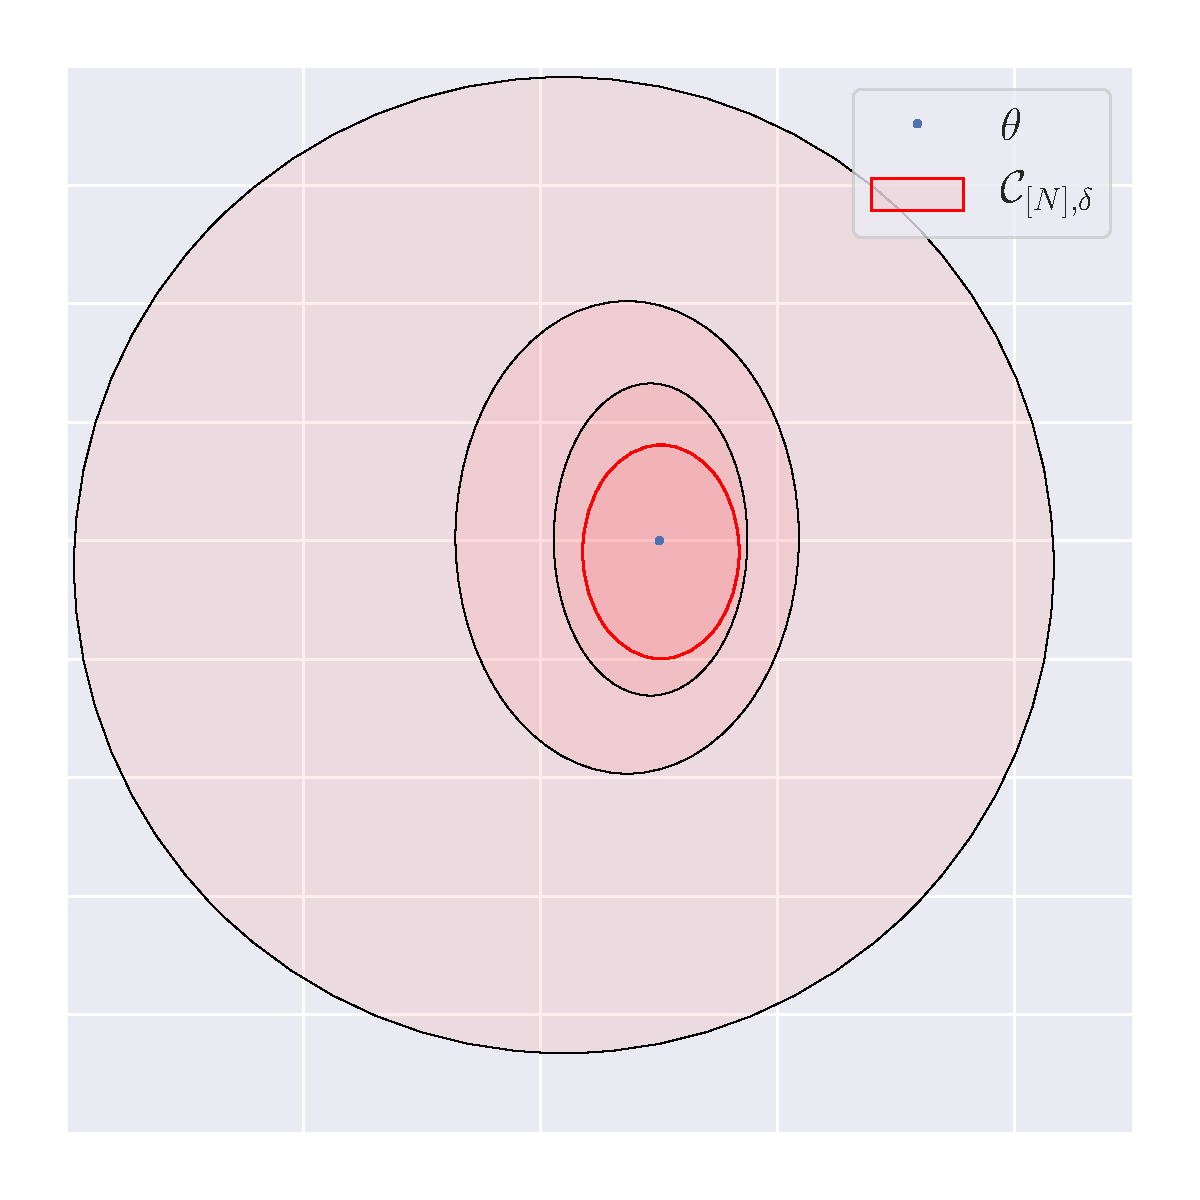
\includegraphics[trim={1cm 0 0 0}, clip, width=0.5\linewidth]{img/ellipsoid}
	\caption{The model estimation procedure. The confidence region $\confidenceset$ shrinks with the number of samples $N$.}
	\label{fig:estimation}
\end{figure}
To address the issue of model bias, we turn to the framework of \emph{robust} decision-making: At time step $N\in\Natural$, instead of merely considering a point estimate of the dynamics, the control scheme needs to rely on an entire \emph{confidence region} $\gls+{confidenceset}$, illustrated in \Cref{fig:estimation}, that contains the true dynamics parameters with high probability:
\begin{align}
\probability{\theta\in \gls+{confidenceset}} \geq 1-\gls+{confidence},
\label{eq:confidence}
\end{align}
where $\confidence\in(0,1]$ is the confidence level. 
In order to derive an explicit form for this confidence region $\confidenceset$, additional assumptions need to be taken regarding the relation between the state transition $\dot{x}$ and its parameter $\theta$. Out of the various hypothesis classes that could represent $f_\theta$, we require one that provides confidence regions for regression. Thus, we make a first assumption that $f_\theta$ is linearly dependent on $\theta$, so as to leverage the statistical tools developed for non-asymptotic linear regression.

\begin{assumption}[Structure \textsc{II}]
	\begin{leftbar}[assumptionbar]
	We assume that $f_\theta$ takes the form
	\begin{equation*}
	\dot{x}(t) = \phi\left(x(t),u(t),\omega(t)\right)\gls+{params} + \psi\left(x(t),u(t),\omega(t)\right),
	\end{equation*}
	where $\phi$ and $\psi$ are known functions that depend on $x(t),u(t),\omega(t)$ but not $\params$.
	\end{leftbar}
\end{assumption}

In \textbf{\Cref{sec:estimation}}, having observed a history $\cD_{[N]} = \{(x_n, y_n,u_n)\}_{n\in[N]}$ of transitions, our first contribution extends the work of \citet{Abbasi2011}, who provide a confidence ellipsoid for the least-square estimator, to our setting of feature matrices rather than feature vectors.

% --- 3. We need to propagate model uncertainty to predicted trajectories -> linear dependency in the states
\paragraph{Propagation of uncertainty}

\begin{figure}[ht]
	\centering
	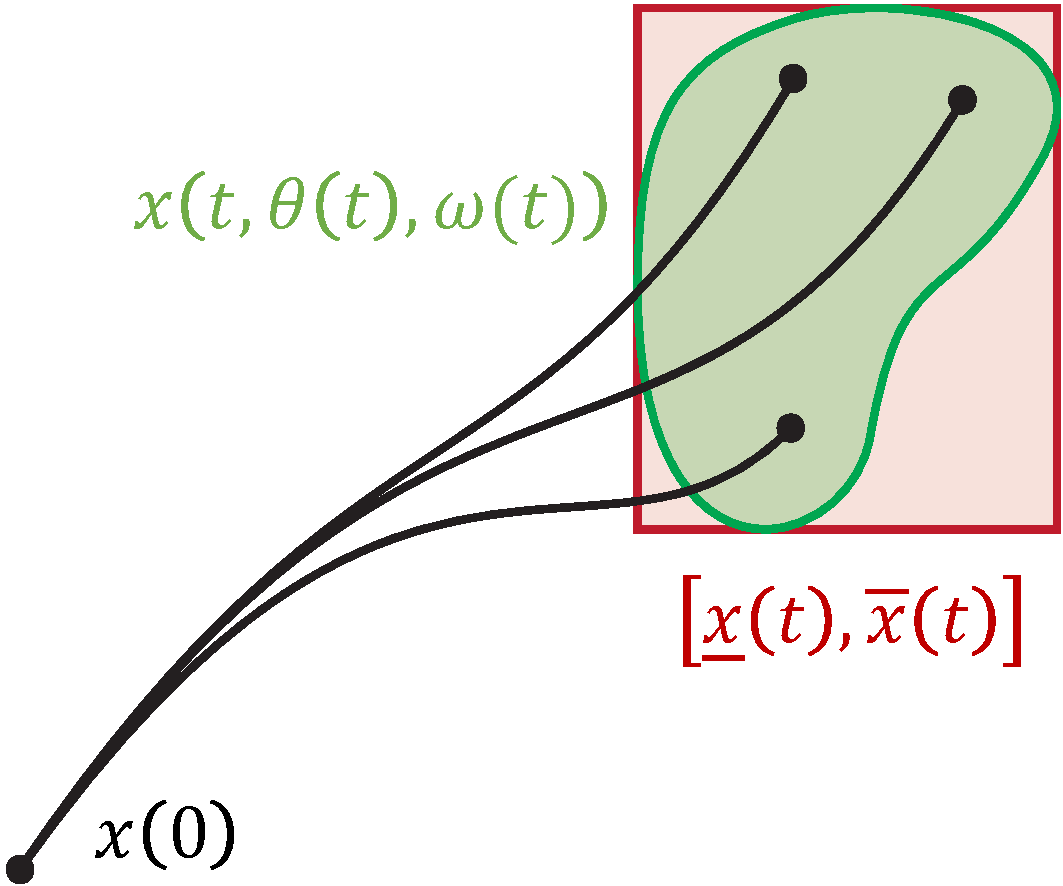
\includegraphics[trim={0 0 0 0}, clip, width=0.5\linewidth]{img/interval-hull}
	\caption{The state prediction procedure. At each time step, we bound the set of reachable states \hlg{$x(t)$ (in green)} under model uncertainty $\confidenceset$ inside the interval \hlr{$[\ux(t), \ox(t)]$ (in red)}.}
	\label{fig:prediction}
\end{figure}

In order to inform the controls, the uncertainty $\confidenceset$ about the dynamics needs to be propagated to the induced trajectories. To that end, we wish to derive an interval predictor $[\ux(t),\ox(t)]$ which takes the information on the current state ${x}_N$, the confidence region $\confidenceset$, a planned control sequence $\bu$ and admissible perturbation bounds $[\underline{\omega}(t),\overline{\omega}(t)]$; and verifies the \emph{inclusion property} illustrated in \Cref{fig:prediction}:
\begin{equation}
\label{eq:inclusion-property}
\gls+{underx}(t)\leq x(t)\leq \gls+{overx}(t),\; \forall t\geq t_N.
\end{equation}
Yet, in order to obtain a closed-form for $[\ux(t),\ox(t)]$, we need to know how the uncertainty over $x(t)$ can affect that of the next state $x(t+dt)$, which requires further specifying the shape of the features $\phi$ and $\psi$. Again, we make an assumption that $\phi$ and $\psi$ are linearly dependent on the states $x(t)$, controls $u(t)$ and perturbations $\omega(t)$, so as to draw on the theory of interval observers for linear systems. Thus, in this chapter we will consider a dynamical system in the following form.

\begin{assumption}[Structure \textsc{III}]
	\label{assumpt:structure}
	\begin{leftbar}[assumptionbar]
		There exists a known feature tensor $\features\in \Real^{d \times p \times p}$ such that for all $\theta\in\Theta$,
		
		\begin{equation}
		\label{eq:dynamics}
		\dot{x}(t)=\gls+{structureddynamics} x(t) + B u(t) + D \omega(t),\;t\geq0,
		\end{equation}
		with
		\begin{equation}
		\gls+{structureddynamics} = A + \sum_{i=1}^d \gls+{params}_i\gls+{features}_i,
		\end{equation}
		where $A,\features_1,\dots,\features_d\in\Real^{p\times p}$ are known. 
	\end{leftbar}
\end{assumption}
For all $n$, we denote $\Phi_n = [\phi_1 x_n \dots \phi_d x_n]\in\Real^{p\times d}$.
The control matrix $B\in\Real^{p\times q}$ and disturbance matrix $D\in\Real^{p\times r}$ are known. We also assume access to the observation of $x(t)$ and to a noisy measurement of $\dot{x}(t)$ in the form 
% We do not take y1,y2 with noise on x for now.
\begin{equation}
\label{eq:outputs}
y(t)=\dot{x}(t) + C\nu(t),
\end{equation}
where $\nu(t)\in\Real^s$ is a measurement noise and $C\in\Real^{p\times s}$ is known. Assumptions over the disturbance $\omega$ and noise $\nu$ will be detailed further, and we denote $\eta(t) = C\nu(t) + D\omega(t)$. 

In \textbf{\Cref{sec:prediction}}, as a second contribution, we derive an \emph{interval predictor} $[\ux(t),\ox(t)]$ for the system \eqref{eq:dynamics}, and analyse its stability.

% --- 4. First application: stabilisation and robust constraint satisfaction
\paragraph{Robust stabilisation and constraint satisfaction}

As a third contribution and first application, we consider the problem of robustly stabilising the system \eqref{eq:dynamics} at a vicinity of the origin under parametric uncertainty and bounded perturbations, while also ensuring that
\begin{equation}
x(t)\in\safestates,\;u(t)\in\safecontrols\quad\forall t\geq0, \label{eq:constraints}
\end{equation}
where $[\ux_{0},\ox_{0}]\subset\safestates\subset\Real^{p}$ and $\safecontrols\subset\Real^{q}$ are given bounded constraint sets for the state and the control, respectively.
In \textbf{\Cref{sec:robust-stabilisation}}, we introduce a Dual-\gls{MPC} scheme that achieves this result by relying on a stabilising control for the predicted intervals $[\ux(t), \ox(t)]$.

% --- 5. Second application: minimax control of generic costs
\paragraph{Minimax control beyond quadratic costs}
Yet, many tasks cannot be framed as stabilisation problems (\eg obstacle avoidance). To achieve more flexible goals, these tasks can be better formulated with the \emph{minimax control objective} \citep{Bental2009,Bertsimas2011,Gorissen2015}, that we consider as a second application. This objective aims to maximise the worst-case return $V^r$ with respect to the confidence region $\confidenceset$ and admissible perturbations
\begin{equation}
\label{eq:minimax-obj}
\hlg{\sup_{\bu\in{(\Real^q)}^\Natural}} \underbrace{\hlr{\inf_{\substack{\theta \in \confidenceset \\ \bom\in[\underline{\bom},\overline{\bom}]^\Natural}}} \left[\sum_{n=N+1}^\infty \gamma^n R(x_n(\bu,\bom))\right]}_{{V^r(\bu)}},
\end{equation}
where $x_n(\bu,\bom)$ is the state reached at step $n$ under controls $\bu$ and perturbations $\bom$ within the given admissible bounds $[\underline\omega(t),\overline\omega(t)]$, and $\R$ is an \emph{arbitrary} bounded reward function. This choice of rich reward space is crucial to have sufficient flexibility to model non-convex and non-smooth functions that naturally arise in many practical problems involving combinatorial optimisation, branching decisions, etc., while quadratic costs are mostly suited for tracking a fixed reference trajectory \citep[\eg][]{Kumar2013}.

Unfortunately, minimax problems such as $\eqref{eq:minimax-obj}$ are already notoriously hard when the reward $\R$ has a simple form. Without a restriction on the shape of functions $\R$, solving the optimal -- not to mention the robust -- control objective is intractable and we cannot hope to derive an explicit solution. Thus, in \textbf{\Cref{sec:control}} we propose a robust \gls{MPC} algorithm for solving \eqref{eq:minimax-obj} numerically. Facing a sequential decision problem with continuous states, we turn to the literature of tree-based planning algorithms studied in \Cref{chapter:6}.
However, these techniques are designed for a single known generative model rather than a confidence region for the system dynamics. We adapt them to the robust objective \eqref{eq:minimax-obj} by approximating it with a tractable surrogate $\hat{V}^r$ that exploits the interval predictions $[\ux(t), \ox(t)]$ to define a pessimistic reward $\underline{R}$. In our main result, we show that the best surrogate performance achieved during planning is guaranteed to be attained on the true system, and provide an upper bound for the approximation gap and simple regret of our framework in \Cref{thm:minimax-regret-bound}. This is our fourth contribution and the first result of this kind for minimax control with generic costs to the best of our knowledge. 

\paragraph{Multi-model extension}
In \textbf{\Cref{sec:multi-model}}, our fifth contribution extends the proposed framework to consider multiple modelling assumptions, while narrowing uncertainty through data-driven model rejection, and still ensuring safety via robust model-selection during planning.

\paragraph{Numerical experiments}
Finally, in \textbf{\Cref{sec:interval-experiments}} we demonstrate the applicability of our approach in two numerical experiments: a simple illustrative example and a more challenging simulation for safe autonomous driving on \textsc{highway-env}.

\subsection{Related Work}

The control of uncertain systems is a long-standing problem, to which a vast body of literature is dedicated. Existing work is mostly concerned with the problem of \emph{stabilisation} around a fixed reference state or trajectory, including approaches such as $\cH_\infty$ control \citep[][]{Basar1996}, sliding-mode control \citep{Lu1997} or system-level synthesis \citep{Dean2019,Dean2018}. This chapter fits in the popular \gls{MPC} framework, for which adaptive data-driven schemes have been developed to deal with model uncertainty \citep{Sastry1990,Tanaskovic2014,Amos2018}, but lack guarantees. The family of tube-MPC algorithms seeks to derive theoretical guarantees of \emph{robust constraint satisfaction}: as in \Cref{sec:robust-stabilisation}, the state $x$ and control $u$ are constrained in a safe region $\safestates\times\safecontrols$ around the origin, often chosen convex \citep{Fukushima2007,Adetola2009,Aswani2013,Turchetta2016,Lorenzen2017,Kohler2019,Lu2019}. Our work in \Cref{sec:robust-stabilisation} mainly differs in that it relies on intervals rather than zonotopes, for simplicity of implementation and computational efficiency.

Moreover, as we argue previously, many tasks cannot be framed as stabilisation problems (\eg obstacle avoidance) and are better addressed with the minimax control objective, which can allow more flexible goal formulations. Minimax control has mostly been studied in two particular instances.

\paragraph{Finite states} Minimax control of finite Markov Decision Processes with uncertain parameters was studied in \citep{Iyengar2005,Nilim2005,Wiesemann2013}, who showed that the main results of Dynamic Programming can be extended to their robust counterparts only when the dynamics ambiguity set verifies a certain rectangularity property. Since we consider continuous states, these methods do not apply.

\paragraph{Linear dynamics and quadratic costs} Several approaches have been proposed for cumulative regret minimisation in the \gls+{LQ} problem. In the \gls+{OFU} paradigm, the best possible dynamics within a high-confidence region is selected under a controllability constraint, to compute the corresponding optimal control in closed-form by solving a Riccati equation. The results of 	\citep{abbasi-yadkori11a,Ibrahimi2013,Faradonbeh2020} show that this procedure achieves a $\tilde{\cO}\left(N^{1/2}\right)$ regret. Posterior sampling algorithms \citep{Ouyang2017,abeille18a} select candidate dynamics randomly instead, and obtain the same result. Other works use noise injection for exploration, such as \citep{Dean2019,Dean2018}. However, neither optimism nor random exploration fits a critical setting, where ensuring safety requires instead to consider pessimistic outcomes. The work of \citet{Dean2019} is close to our setting: after an offline estimation phase, they estimate a simple regret between a minimax controller and the optimal performance. Our work differs in that it addresses a generic shape cost. 
Another work of interest is that of \citet{Rosolia2019} where worst-case generic costs are considered. However, they assume knowledge of the dynamics, and their rollout-based solution only produces inner-approximations and does not yield any guarantee. In this chapter, interval prediction is used to produce oversets, while a near-optimal control is found using a tree-based planning procedure.


\section{Confident model estimation}
\label{sec:estimation}

The goal of this section is to derive a confidence region \eqref{eq:confidence} for the parameters $\theta$ of the dynamics \eqref{eq:dynamics}.

We abuse notations and define a virtual measurement signal, still denoted $y(t)$, that includes additional known terms
\begin{equation*}
%\label{eq:measurement}
y(t) = \dot{x}(t) + C\nu(t) - A x(t) - Bu(t),
\end{equation*}
to obtain a linear regression system
$
y_n = \Phi_n\theta + \eta_n.
$

\paragraph{Regularised least square} To derive an estimate on $\theta$, we consider the weighted $L_2$-regularised regression problem with weights $\Sigma_p\in\Real^{p\times p}$ and parameter $\lambda\in\Real^+_*$:
\begin{equation}
\label{eq:regression_min}
\min_{\theta\in\Real^d} \sum_{n=1}^N \|y_n -\Phi_n\theta\|_{\Sigma_p^{-1}}^2 + \lambda\|\theta\|_{}^2.
\end{equation}


The solution can be obtained as:

\begin{proposition}[Regularised solution]
	\label{prop:regularized_solution}
	\begin{leftbar}[propositionbar]
	The solution to \eqref{eq:regression_min} is
	\begin{align}
	\label{eq:vector_rls}
	\gls+{lse} &\eqdef G_{N, \lambda}^{-1} \sum_{n=1}^N \Phi_n^\transp \Sigma_p^{-1} y_n,\\
	\label{eq:g_n_lambda}
	\text{where }\quad \gls+{gramian} &\eqdef \sum_{n=1}^N \Phi_{n}^\transp\Sigma_p^{-1}\Phi_{n}  + \lambda I_d \in \Real^{d\times d}.
	\end{align}
	\end{leftbar}
\end{proposition}
\begin{proof}
	We provide a proof in \Cref{sec:proof-regularized_solution}.
\end{proof}

Substituting $y_n$ into \eqref{eq:vector_rls} yields the regression error
\begin{align}
\theta_{N,\lambda} - \theta = G_{N, \lambda}^{-1}\sum_{n=1}^N \Phi_n^\transp \Sigma_p^{-1}\eta_n - \lambda G_{N, \lambda}^{-1}\theta.
\end{align}


Depending on the assumption we have over the noise $\eta_n$, we can bound this error in different ways.


\subsection{Bounded noise}

\begin{assumption}[Bounded noise]
\label{assumpt:bounded-noise}
\begin{leftbar}[assumptionbar]
The noise $\eta(t)$ is bounded in $\|\cdot\|_\infty$.
	
More precisely, we assume that there exists known signals $\underline{\omega},\overline{\omega}\in\cL_{\infty}^{r}$ such that $\underline{\omega}(t)\leq \omega(t)\leq\overline{\omega}(t)$ for all $t\geq0$.
\end{leftbar}
\end{assumption}

This is a deterministic assumption, then by Hölder inequality a confidence region $\cC_{[N],0}$ can be derived based on a $L_1$-ball estimate of $\theta$ at time $N$, \ie a polytope with $2d$ vertices
\begin{equation}
\label{eq:bounded-noise-polytope}
\|\theta_{N,\lambda}\! -\! \theta\|_1\! \leq \! \|G_{N, \lambda}^{-1}\!\sum_{n=1}^N \!\Phi_n^\transp\! \Sigma_p^{-1}\!\|_1\|\eta\|_\infty\! +\!\lambda\|G_{N, \lambda}^{-1}\!\|_1S
\end{equation}

\subsection{Sub-Gaussian noise}

There may be cases where \Cref{assumpt:bounded-noise} does not hold. For instance, when the noise $\eta$ is Gaussian, then $\|\eta\|_\infty=+\infty$ which makes \eqref{eq:bounded-noise-polytope} uninformative. Then, another probabilistic assumption can be made.

\begin{assumption}[Sub-Gaussian Noise]
	\label{assumpt:gaussian-noise}
	\begin{leftbar}[assumptionbar]
	At each time $t\geq0$ the noise $\eta(t)$ is an independent sub-Gaussian noise with covariance proxy $\Sigma_p \in \Real^{p\times p}$:
	\begin{equation*}
	\forall u\in\Real^p,\, \expectedvalue \left[ \exp{\left( u^\transp \eta(t)\right)}\right] \leq \exp{\left( \frac{1}{2} u^\transp \Sigma_p u\right)}.
	\end{equation*}
	\end{leftbar}
\end{assumption}
For instance, it is the case when $\nu$ and $\omega$ are Gaussian noises with covariance matrices $\Sigma_r$ and $\Sigma_s$, with $\Sigma_p \eqdef C\Sigma_r C^\transp + D\Sigma_s D^\transp$. Note that \Cref{assumpt:bounded-noise} implies that $\eta$ is sub-Gaussian with covariance proxy $\Sigma_p=\|\eta\|_\infty I_p$.

\begin{remark}
	\begin{leftbar}[remarkbar]
		The robust objective \eqref{eq:minimax-obj} involves bounds $\underline{\omega}(t)\leq \omega(t) \leq \overline{\omega}(t)$ over the possible perturbations we want to protect against. In the unbounded sub-Gaussian noise setting of \Cref{assumpt:gaussian-noise}, we can use the same formulation by deriving local high-confidence bounds that each holds with confidence $\confidence_n$. By choosing $\confidence_n = \frac{\confidence}{n(n+1)}$, the event $\{\forall n, \underline{\omega}(t_n) \leq \omega(t_n) \leq \overline{\omega}(t_n)\}$ holds with probability $1-\confidence$.
	\end{leftbar}
\end{remark}

Under this assumption, we can derive a confidence ellipsoid for $\params$.

\begin{theorem}[Confidence ellipsoid, a matricial version of \citealp{Abbasi2011}]
	\label{thm:confidence_ellipsoid}
	\begin{leftbar}[theorembar]
	Under \Cref{assumpt:gaussian-noise}, it holds with probability at least $1-\confidence$ that
	\begin{align}
	\label{eq:confidence-ellipsoid}
	\| \theta_{N,\lambda}  - \theta\|_{G_{N,\lambda}} \leq \beta_N(\confidence),
	\end{align}
	with
	\begin{equation}
	\label{eq:beta_n}
	\beta_N(\confidence)\eqdef \sqrt{2\log \left(\frac{\det(G_{N,\lambda})^{1/2}}{\confidence\det(\lambda I_d)^{1/2}}\right)}
	+ (\lambda d)^{1/2}\|\theta\|_\infty.
	\end{equation}
	\end{leftbar}
\end{theorem}
\begin{proof}
	We provide a proof in \Cref{sec:proof-confidence_ellipsoid}.
\end{proof}

\section{State interval prediction}

\label{sec:prediction}

%There are plenty of emerging application domains nowadays, where the decision algorithms have to operate in the conditions of severe uncertainty. In most of these applications, even the nominal simplified models are nonlinear, and in order to solve the problem of estimation and control in nonlinear and uncertain systems, a popular approach is based on the Linear Parameter-Varying (LPV) representation of their dynamics \citep{Shamma2012,Marcos_Balas04,Shamma_Cloutier93,Tan97}, since it allows to reduce the problem to the linear context at the price of augmented parametric variation.

In this section, we view our dynamics \eqref{eq:dynamics} of \Cref{assumpt:structure} as an instance of the more general context of the \gls{LPV} representation of the dynamics \citep{Shamma2012,Marcos_Balas04,Shamma_Cloutier93,Tan97}
\begin{equation}
\dot{x}(t)=A(\hlrb{\theta(t)})x(t)+ Bu(t) + D\omega(t),\;t\geq0,\label{eq:LPV_syst}
\end{equation}
where the (known) matrix function $A:\Theta\to\Real^{n\times n}$ is only locally bounded (continuous) and does not have to be linear in $\theta$, and where unknown parameters $\theta(t)$ are free to evolve within the known set of admissible values $\Theta$, $\theta\in\cL_{\infty}^{d}$. 

Moreover, we assume that \Cref{assumpt:bounded-noise} is verified, such that the input $\omega(t)$ belongs to a known bounded interval $[\underline{\omega}(t),\overline{\omega}(t)]$ for all $t\in\Real_{+}$, which is the standard hypothesis for interval estimation \citep{Efimov2016,Raiessi2018}. We also suppose in the following  \Cref{assumpt:bounded-state} that the system \eqref{eq:LPV_syst} generates stable trajectories with a bounded state $x$ for the applied class of inputs $u(t),\,\omega(t)$, and the initial conditions $x(0)$ are constrained to belong to a given interval $[\ux_{0},\ox_{0}]$.
\begin{assumption}[Bounded state]
	\label{assumpt:bounded-state}
	\begin{leftbar}[assumptionbar]
		In the system \eqref{eq:LPV_syst}, $x\in\cL_{\infty}^{n}$. 
		
		In addition, $x(0)\in[\ux_{0},\ox_{0}]$ for some known $\ux_{0},\ox_{0}\in\Real^{n}$.
	\end{leftbar}
\end{assumption}

Note that since the function $A$ and the set $\Theta$ are known, and $\theta\in\Theta$, then there exist matrices $\underline{A},\overline{A}\in\Real^{p\times p}$, which can be easily computed, such that 
\[
\underline{A}\leq \structureddynamics\leq\overline{A},\quad\forall\theta\in\Theta.
\]

The objective of this section is to design an \emph{interval predictor} for the system \eqref{eq:LPV_syst}, which takes the information on the initial conditions $[\ux_{0},\ox_{0}]$, the admissible bounds on the values of the exogenous input $[\underline{\omega}(t),\overline{\omega}(t)]$, the information about $A(\cdot)$ and $\Theta$ (\eg the matrices $\underline{A},\overline{A}$, but not the instant value of $\theta(t)$) and generates bounded interval estimates $\ux(t),\ox(t)\in\Real^{p}$ such that
\begin{equation}
\gls+{underx}(t)\leq x(t)\leq\gls+{overx}(t),\quad\forall t\geq0.\tag{\ref{eq:inclusion-property}}
\end{equation}

In the presence of uncertainty (unknown parameters $\params$ or/and external disturbances $\omega(t)$) the design of a conventional estimator or predictor, approaching the ideal value of the state, can be realised under restrictive assumptions only. However, an interval estimation/prediction remains frequently feasible: using input-output information an algorithm evaluates the set of admissible values (interval) for the state at each instant of time \citep{Efimov2016,Raiessi2018}. The interval length must be minimised via a parametric tuning of the system, and it is typically proportional to the size of the model uncertainty \citep{Chebotarev2015}. It is worth stressing that the interval estimation or prediction is not a relaxation of the original problem, in fact it is an improvement since the interval mean value can be used as the state pointwise estimate, while the interval bounds provide a simultaneous accuracy evaluation for given uncertainty.

There are many approaches to design interval/set-membership estimators and predictors \citep{Jaulin02,Kieffer2004,Bernard_Gouze04,Moisan_Bernard_Gouze09}, and this section focuses on the design based on the monotone systems theory \citep{Bernard_Gouze04,Moisan_Bernard_Gouze09,RVZ10,REZ11,Efimov2012}.
In such a way the main difficulty for synthesis consists in ensuring cooperativity of the interval error dynamics by a proper design of the algorithm. As it has been shown in \citep{MazencBernard11,REZ11,Combastel2012}, such a complexity of the design can be handled by applying an additional transformation of coordinates, which maps a stable system into a stable and monotone one. An approach for selection of a constant similarity transformation matrix representing a given interval of matrices to an interval of Metzler matrices (providing monotonicity) has been developed in \citep{Efimov_a2013,Chebotarev2015}. 

When designing a predictor, the main difficulty to overcome is the predictor stability, which contrarily to an observer cannot be imposed by a proper design of the gains. An interval inclusion of the uncertain components can be restrictive and transform an initially stable system to an unstable one. In other words, an important problem is to keep the interval predictor stability in the presence of uncertainties and saving the interval inclusion property of the estimates, then an unstable system can definitely enclose the trajectories of a stable one, but at the price of precision. To solve this problem, first, a generic predictor is proposed for an \gls{LPV} system, whose estimates can be combined with the interval frequency-based estimator presented earlier. To analyse the stability of the predictor, which is modelled by a nonlinear Lipschitz dynamics, a novel non-conservative Lyapunov function is developed, whose features can be verified through solution of \glspl{LMI}. Second, we revisit the case of \gls{LTI} models and demonstrate an asymptotic accuracy improvement that can be achieved if a piece of  additional information about external signals is given: the admissible interval of frequency spectrum. Finally, the utility of the developed theory is demonstrated with a safe motion planning application on \highwayenv.

The section is organised as follows: in \Cref{sec:interval-preliminaries}, we start by giving an introduction to the theory of interval estimation for \gls{LTI} systems, before considering a motivating example. An improved interval predictor is presented in \Cref{sec:Main-results}. The asymptotic accuracy is enhanced using frequency-based estimation in \Cref{sec:Frequency}. Application of the developed theory to the problem of path planning for an autonomous vehicle is shown in \Cref{sec:interval-prediction-experiments}.

\subsection{Preliminaries}
\label{sec:interval-preliminaries}

We first give some background on interval arithmetic and nonnegative systems, before considering a motivating example.

\subsubsection{Interval arithmetic}

\begin{lemma}[\citealp{Efimov2012}]
	\label{lem:interval}
	Let $x\in\mathbb{R}^{n}$ be a vector variable, $\ux\le x\le\ox$ for some $\ux,\ox\in\mathbb{R}^{n}$. 
	
	\textup{(1)} If $A\in\Real^{m\times n}$ is a constant matrix, then
	\begin{equation}
	A^{+}\ux-A^{-}\ox\le Ax\le A^{+}\ox-A^{-}\ux.\label{eq:Interval1}
	\end{equation}
	
	\textup{(2)} If $A\in\Real^{m\times n}$ is a matrix variable and \textup{$\underline{A}\le A\le\overline{A}$} for some $\underline{A},\overline{A}\in\Real^{m\times n}$, then
	\begin{gather}
	\underline{A}^{+}\ux^{+}-\overline{A}^{+}\ux^{-}-\underline{A}^{-}\ox^{+}+\overline{A}^{-}\ox^{-}\leq Ax\label{eq:Interval2}
	\leq\overline{A}^{+}\ox^{+}-\underline{A}^{+}\ox^{-}-\overline{A}^{-}\ux^{+}+\underline{A}^{-}\ux^{-}. 
	\end{gather}
\end{lemma}
Furthermore, if $-\overline{A}=\underline{A}\le0\le\overline{A}$, then the inequality \eqref{eq:Interval2} can be simplified: $$-\overline{A}(\ox^{+}+\ux^{-})\leq Ax\leq\overline{A}(\ox^{+}+\ux^{-}).$$

\subsubsection{Nonnegative systems}

\begin{definition}[Hurwitz]
	\begin{leftbar}[defnbar]
		A matrix $A\in\Real^{n\times n}$ is called {Hurwitz} if all its eigenvalues have negative real parts, 
	\end{leftbar}
\end{definition}
\begin{definition}[Metzler]
	\begin{leftbar}[defnbar]
		A matrix $A\in\Real^{n\times n}$ is called {Metzler} if all its elements outside the main diagonal are nonnegative.
	\end{leftbar}
\end{definition}

Any solution of the \gls{LTI} system
\begin{gather}
\dot{x}(t)=Ax(t)+Bu(t)+ D\omega(t),\:t\geq0,\label{eq:LTI_syst}\\
y(t)=Cx(t)+E\omega(t),\nonumber 
\end{gather}
with $x(t)\in\Real^{n}$, $y(t)\in\Real^{p}$ and a Metzler matrix $A\in\Real^{p\times p}$, is elementwise nonnegative for all $t\ge0$ provided that $x(0)\ge0$, $u:\Real_{+}\to\Real_{+}^{q}$, $\omega:\Real_{+}\to\Real_{+}^{r}$ and $B\in\Real_{+}^{p\times q}$, $D\in\Real_{+}^{p\times r}$ \citep{FarinaRinaldi2000,Smith95}. The output solution $y(t)$ is nonnegative if $C\in\Real_{+}^{s\times p}$ and $E\in\Real_{+}^{s\times r}$. Such dynamical systems are called cooperative (monotone) or nonnegative if only initial conditions in $\Real_{+}^{n}$ are considered \citep{FarinaRinaldi2000,Smith95}.

\begin{lemma}[\citealp{REZ11}]
	\label{lem:l2}
	\begin{leftbar}[lemmabar]
		Given the matrices $A\in\Real^{p\times p}$, $Y\in\Real^{p\times p}$ and \textup{$C\in\Real^{s\times p}$. }If there is a matrix \textup{$L\in\Real^{p\times s}$} such that the matrices $A-LC$ and $Y$ have the same eigenvalues, then there is a matrix $S\in\Real^{p\times p}$ such that $Y=S(A-LC)S^{-1}$ provided that the pairs $(A-LC,\chi_{1})$ and $(Y,\chi_{2})$ are observable for some $\chi_{1}\in\Real^{1\times p}$, $\chi_{2}\in\Real^{1\times p}$.
	\end{leftbar}
\end{lemma}
This result allows to represent the system \eqref{eq:LTI_syst} in its nonnegative form via a similarity transformation of coordinates.
\begin{lemma}[\citealp{Efimov_a2013}]
	\label{lem:l3}
	\begin{leftbar}[lemmabar]
		Let $D\in\Xi\subset\Real^{p\times p}$ be a matrix variable satisfying the interval constraints $\Xi=\{D\in\Real^{p\times p}:\,D_{a}-\Delta\le D\le D_{a}+\Delta\}$ for some $D_{a}^{\text{T}}=D_{a}\in\Real^{p\times p}$ and $\Delta\in\Real_{+}^{p\times p}$. If for some constant $\mu\in\Real_{+}$ and a diagonal matrix $\Upsilon\in\Real^{p\times p}$ the Metzler matrix $Y=\mu E_{p\times p}-\Upsilon$ has the same eigenvalues as the matrix $D_{a}$, then there is an orthogonal matrix $S\in\Real^{p\times p}$ such that the matrices $S^{\text{T}}DS$ are Metzler for all $D\in\Xi$ provided that $\mu>p||\Delta||_{max}$.\textup{ }
	\end{leftbar}
\end{lemma}
In the last lemma, the existence of similarity transformation is proven for an interval of matrices, \emph{e.g}. in the case of \gls{LPV} dynamics.


\subsubsection{A motivating example}

Following the result of \Cref{lem:interval}, there is a straightforward solution to the problem:


\begin{proposition}
	\label{prop:interval-predictor-naive}
	\begin{leftbar}[propositionbar]
		Let \Cref{assumpt:bounded-noise,assumpt:bounded-state} be satisfied for the system \eqref{eq:LPV_syst}, then the interval predictor
		\begin{align}
		\label{eq:predictor-naive}
		\begin{split}
		\dot{\ux}(t) = {} & \underline{A}^{+}\ux^{+}(t)-\overline{A}^{+}\ux^{-}(t)-\underline{A}^{-}\ox^{+}(t) +\overline{A}^{-}\ox^{-}(t) + Bu(t)+D^{+}\underline{\omega}(t)-D^{-}\overline{\omega}(t),\\
		\dot{\ox}(t) =  {} & \overline{A}^{+}\ox^{+}(t)-\underline{A}^{+}\ox^{-}(t)-\overline{A}^{-}\ux^{+}(t) +\underline{A}^{-}\ux^{-}(t) + Bu(t) +D^{+}\overline{\omega}(t)-D^{-}\underline{\omega}(t), \\
		\text{with }\, & \ux(0)=  \ux_{0},\;\ox(0)=\ox_{0}, 
		\end{split}
		\end{align}
		ensures the inclusion property \eqref{eq:inclusion-property}. 
	\end{leftbar}
\end{proposition}
\begin{proof}
	The relations \eqref{eq:inclusion-property} can easily be obtained by recursively applying \Cref{lem:interval} at each time step.
\end{proof}
Unfortunately, the stability analysis of the system \eqref{eq:predictor-naive} is more tricky. Indeed, \eqref{eq:predictor-naive} is a purely nonlinear system (since $\ux^{+}$, $\ux^{-}$, $\ox^{+}$ and $\ox^{-}$ are globally Lipschitz functions of the state $\ux$ and $\ox$), whose robust stability with respect to the bounded external inputs $\underline{\omega}$ and $\overline{\omega}$ can be assessed if a suitable Lyapunov function is found. And it is easy to find an example, where the matrices $\underline{A}$ and $\overline{A}$ are stable, but the system \eqref{eq:predictor-naive} is not:
\begin{example*}[motivating]
	\begin{figure}[t]
		\begin{centering}
			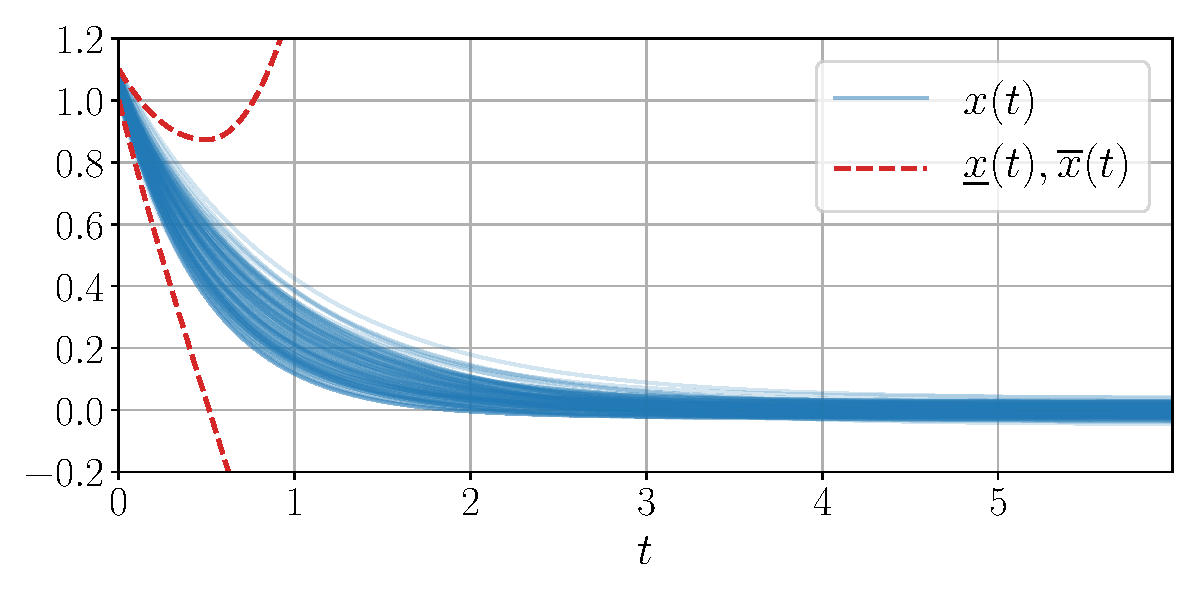
\includegraphics[width=0.8\linewidth]{img/observer}
			\par\end{centering}
		\caption{\label{fig:IP_Direct} The results of prediction by \eqref{eq:predictor-naive}: even in such a simplistic setting, the predictor is unstable and diverges quickly.}
	\end{figure}
	Consider a scalar system
	\[
	\dot{x}(t)=-\theta(t)x(t)+\omega(t),\;t\geq0,
	\]
	where $x(t)\in\Real$ with $x(0)\in[\ux_{0},\ox_{0}]=[1.0, 1.1]$, $\theta(t)\in\Theta=[\underline{\theta},\overline{\theta}]=[0.5,1.5]$ and $\omega(t)\in[\underline{\omega},\overline{\omega}]=[-0.1,0.1]$ for all $t\geq0$. Obviously, \Cref{assumpt:bounded-noise,assumpt:bounded-state} are satisfied, and this uncertain dynamics produces bounded trajectories (to prove this consider a Lyapunov function $V(x)=x^{2}$). Then the interval predictor \eqref{eq:predictor-naive} takes the form
	\begin{align*}
		\dot{\ux}(t) & = -\overline{\theta}\ox^{+}(t)+\underline{\theta}\ox^{-}(t)+\underline{\omega},\\
		\dot{\ox}(t) & = -\underline{\theta}\ux^{+}(t)+\overline{\theta}\ux^{-}(t)+\overline{\omega}.
	\end{align*}
	The results of simulation are shown in \Cref{fig:IP_Direct}. As we can conclude, additional consideration and design are needed to properly solve the posed problem.
\end{example*}

\subsection{Interval predictor design}
\label{sec:Main-results}

Note that, in related papers \citep{AitRami2008,RVZ10,Bolajraf2011,Efimov_a2013,Efimov_tac2013,Chebotarev2015}, various interval observers for \gls{LPV} systems have been proposed, but in those works the cooperativity and stability of the estimation error dynamics are ensured by a proper selection of observer gains and/or by design of control algorithms, which can be dependent on $\ux$, $\ox$ and guarantee the observer robust stability. For an interval predictor there is no such a freedom, and a careful selection of hypotheses has to be made in order to provide a desired solution.
We will additionally assume the following:
\begin{assumption}
	\label{assumpt:polytope}
	\begin{leftbar}[assumptionbar]
	There exist a matrix $A_{0}\in\Real^{p\times p}$ and matrices $\Delta A_{i}\in\Real^{p\times p}$, $i\in[M]$ for some $M\in\Natural_{+}$ such that the following relations are satisfied for all $\theta\in\Theta$:
	\begin{gather*}
	\structureddynamics=A_{0}+\sum_{i=1}^{M}\lambda_{i}(\theta)\Delta A_{i},\\
	\sum_{i=1}^{M}\lambda_{i}(\theta)=1;\;\lambda_{i}(\theta)\in[0,1],\;i\in[M].
	\end{gather*}
	\end{leftbar}
\end{assumption}
Therefore, it is assumed that the matrix $\structureddynamics$ for any $\theta\in\Theta$ can be embedded in a polytope defined by $M$ known vertices $\Delta A_{i}$ with the given centre $A_{0}$. 

To connect this assumption to the results obtained from model estimation in previous section, we can enclose the confidence ellipsoid $\confidenceset$ on $\theta$ obtained from $\eqref{eq:confidence-ellipsoid}$ at time $t=t_N$ into a polytope $\cP$ on $\structureddynamics$. For simplicity, we present here a simple but coarse strategy: bound the ellipsoid by its enclosing sphere, and then the sphere by its enclosing hypercube. We obtain
\begin{align}
\label{eq:polytope}
&\cP = \left\{ A_{0}+\sum_{i=1}^{M}\lambda_{i}\Delta A_{i}: \lambda\geq 0,  \sum_{i=1}^{M}\lambda_{i}=1\right\},
\end{align}
where 
\begin{alignat*}{4}
&A_{0}&&=A + \theta_{N,\lambda}^\transp\phi, & \hspace{4em}
&M &&= 2^d\\
&\Delta A_{i}&&= \sqrt{\frac{\beta_N(\confidence)}{\lambda_{\max}(G_{N,\lambda})}}{h_i}^\top\phi,& 
&h_i&&\in\{-1,1\}^d.
\end{alignat*}
Another strategy presented in \Cref{sec:tight-polytope} produces a much tighter polytope, at the price of an increased computational cost required by the diagonalisation of $G_{N,\lambda}$.

For the given centre $A_0$ to admit useful properties of nonnegative systems, we will further require that it is Metzler. More precisely, according to the results of \Cref{lem:l2,lem:l3}, this can be imposed by applying a properly designed similarity transformation, which maps a matrix (interval of matrices) to a Metzler one. Design of such a transformation is not considered in this chapter, and we will just suppose the following:
\begin{assumption}
	\begin{leftbar}[assumptionbar]
	\label{assumpt:metzler}
	There exists a nonsingular matrix $Z\in\Real^{p\times p}$ such that $Z^{-1}A_{0}Z$ is Metzler.
	\end{leftbar}
\end{assumption}
In practice, this assumption is often verified. It is for instance the case whenever $A_{0}$ is diagonalizable, or a method from \cite{Efimov2013} computes a similarity transformation $Z$ when the system is observable with respect to a scalar output. To simplify the notation, we further assume that $Z=I_{p}$ so that the system \eqref{eq:LPV_syst} has already been put in the right form:
\[
\dot{x}(t)=[A_{0}+\sum_{i=1}^{M}\lambda_{i}(\theta(t))\Delta A_{i}]x(t)+Bu(t) + D\omega(t).
\]
Denote
\[
\Delta A_{+}=\sum_{i=1}^{M}\Delta A_{i}^{+},\;\Delta A_{-}=\sum_{i=1}^{M}\Delta A_{i}^{-},
\]
then the following interval predictor can be designed:
\begin{theorem}
	\label{thm:interval-predictor-main}
	\begin{leftbar}[theorembar]
	Let \Cref{assumpt:bounded-noise,assumpt:bounded-state,assumpt:polytope,assumpt:metzler} be satisfied for the system \eqref{eq:LPV_syst}, then an interval predictor
	\begin{align}
	\label{eq:interval-predictor}
	\begin{split}
	\dot{\ux}(t) = {} & A_{0}\ux(t)-\Delta A_{+}\ux^{-}(t)-\Delta A_{-}\ox^{+}(t) +Bu(t) +D^{+}\underline{\omega}(t)-D^{-}\overline{\omega}(t),\\
	\dot{\ox}(t) = {} & A_{0}\ox(t)+\Delta A_{+}\ox^{+}(t)+\Delta A_{-}\ux^{-}(t)  +Bu(t) +D^{+}\overline{\omega}(t)-D^{-}\underline{\omega}(t), \\
	\text{with }\, & \ux(0)=\ux_{0},\;\ox(0)=\ox_{0} 
	\end{split}
	\end{align}
	ensures the inclusion property \eqref{eq:inclusion-property}. 
	If there exist diagonal matrices $P$, $Q$, $Q_{+}$, $Q_{-}$, $Z_{+}$, $Z_{-}$, $\Psi_{+}$, $\Psi_{-}$, $\Psi$, $\Gamma\in\Real^{2p\times2p}$ such that the following LMIs are satisfied:
	\begin{gather*}
	P+\min\{Z_{+},Z_{-}\}>0,\;\Upsilon\preceq0,\;\Gamma>0,\\
	Q+\min\{Q_{+},Q_{-}\}+2\min\{\Psi_{+},\Psi_{-}\}>0,
	\end{gather*}
	where{
		\begin{gather*}
		\Upsilon=\left[\begin{array}{cccc}
		\Upsilon_{11} & \Upsilon_{12} & \Upsilon_{13} & P\\
		\Upsilon_{12}^{\top} & \Upsilon_{22} & \Upsilon_{23} & Z_{+}\\
		\Upsilon_{13}^{\top} & \Upsilon_{23}^{\top} & \Upsilon_{33} & Z_{-}\\
		P & Z_{+} & Z_{-} & -\Gamma
		\end{array}\right],\\
		\Upsilon_{11}=\mathcal{A}^{\top}P+P\mathcal{A}+Q,\;\Upsilon_{12}=\mathcal{A}^{\top}Z_{+}+PR_{+}+\Psi_{+},\\
		\Upsilon_{13}=\mathcal{A}^{\top}Z_{-}+PR_{-}+\Psi_{-},\;\Upsilon_{22}=Z_{+}R_{+}+R_{+}^{\top}Z_{+}+Q_{+},\\
		\Upsilon_{23}=Z_{+}R_{-}+R_{+}^{\top}Z_{-}+\Psi,\;\Upsilon_{33}=Z_{-}R_{-}+R_{-}^{\top}Z_{-}+Q_{-},\\
		\mathcal{A}=\left[\begin{array}{cc}
		A_{0} & 0\\
		0 & A_{0}
		\end{array}\right],\;R_{+}=\left[\begin{array}{cc}
		0 & -\Delta A_{-}\\
		0 & \Delta A_{+}
		\end{array}\right],\;R_{-}=\left[\begin{array}{cc}
		\Delta A_{+} & 0\\
		-\Delta A_{-} & 0
		\end{array}\right],
		\end{gather*}
	}then the predictor \eqref{eq:interval-predictor} is input-to-state stable with respect to the inputs $\underline{\omega}$, $\overline{\omega}$.
\end{leftbar}
\end{theorem}
Note the requirement that the matrix $P$ has to be diagonal is not restrictive, since for a Metzler matrix $\mathcal{A}$, its stability is equivalent to existence of a diagonal solution $P$ of the Lyapunov equation $\mathcal{A}^{\top}P+P\mathcal{A}\prec0$ \citep{FarinaRinaldi2000}.
\begin{proof}
	First, let us demonstrate \eqref{eq:inclusion-property}, to this end note that
	\[
	-\Delta A_{i}^{-}\leq\lambda_{i}\Delta A_{i}=\lambda_{i}\Delta A_{i}^{+}-\lambda_{i}\Delta A_{i}^{-}\leq\Delta A_{i}^{+}
	\]
	for any $\lambda_{i}\in[0,1],$ then using \Cref{lem:interval} we obtain
	\[
	-\Delta A_{i}^{+}\ux^{-}-\Delta A_{i}^{-}\ox^{+}\leq\lambda_{i}\Delta A_{i}x\leq\Delta A_{i}^{+}\ox^{+}+\Delta A_{i}^{-}\ux^{-}
	\]
	provided that $\ux\leq x\leq\ox$. Hence,
	\[
	-\Delta A_{+}\ux^{-}-\Delta A_{-}\ox^{+}\leq\sum_{i=1}^{N}\lambda_{i}\Delta A_{i}x\leq\Delta A_{+}\ox^{+}+\Delta A_{-}\ux^{-}
	\]
	and introducing usual interval estimation errors $\underline{e}=x-\ux$ and $\overline{e}=\ox-x$ and calculating their dynamics we get:
	\begin{align*}
		\dot{\underline{e}}(t) & = A_{0}\underline{e}(t)+\underline{r}_{1}(t)+\underline{r}_{2}(t),\\
		\dot{\overline{e}}(t) & = A_{0}\overline{e}(t)+\overline{r}_{1}(t)+\overline{r}_{2}(t),
	\end{align*}
	where
	\begin{align*}
	\underline{r}_{1}&=\sum_{i=1}^{M}\lambda_{i}\Delta A_{i}x+\Delta A_{+}\ux^{-}+\Delta A_{-}\ox^{+},\\
	\underline{r}_{2}&=D\omega-D^{+}\underline{\omega}+D^{-}\overline{\omega},\\
	\overline{r}_{1}&=-\sum_{i=1}^{M}\lambda_{i}\Delta A_{i}x+\Delta A_{+}\ox^{+}+\Delta A_{-}\ux^{-},\\
	\overline{r}_{2}&=D^{+}\overline{\omega}-D^{-}\underline{\omega}-D\omega.
	\end{align*}
	Non-negativity or $\underline{r}_{2}$ and $\overline{r}_{2}$ follows from \Cref{assumpt:bounded-noise} and \Cref{lem:interval}. The signals $\underline{r}_{1}$ and $\overline{r}_{1}$ are also nonnegative provided that \eqref{eq:inclusion-property} holds and due to the calculations above. Note that the relations \eqref{eq:inclusion-property} are satisfied for $t=0$ by construction and \Cref{assumpt:bounded-state}, then since the matrix $A_{0}$ is Metzler by \Cref{assumpt:polytope}, we have that $\dot{\underline{e}}_{i}(0)\in\Real_{+}^{p}$ or $\dot{\overline{e}}_{i}(0)\in\Real_{+}^{p}$ provided that $e_{i}(0)=0$ or $e_{i}(0)=0$, respectively, for any $i\in[p]$ (the error cannot become negative). Next, repeating these arguments it is possible to show that $\underline{e}(t)\geq0$ and $\overline{e}(t)\geq0$ for all $t\geq0$ \citep{Smith95}, which confirms the relations \eqref{eq:inclusion-property}.
	
	Second, let us consider the stability of \eqref{eq:interval-predictor}, and for this purpose define the extended state vector as $X=[\ux^{\top}\;\;\ox^{\top}]^{\top}$, whose dynamics admit the differential equation
	\[
	\dot{X}(t)=\mathcal{A}X(t)+R_{+}X^{+}(t)-R_{-}X^{-}(t)+\confidence(t),
	\]
	where
	\begin{gather*}
	\confidence(t)=\left[\begin{array}{cc}
	-D^{-} & D^{+}\\
	D^{+} & -D^{-}
	\end{array}\right]\left[\begin{array}{c}
	\overline{\omega}(t)\\
	\underline{\omega}(t)
	\end{array}\right]
	\end{gather*}
	is a bounded input vector, whose norm is proportional to $\underline{\omega}$,
	$\overline{\omega}$. Consider a candidate Lyapunov function
	\begin{gather*}
	V(X)=X^{\top}PX+X{}^{\top}Z_{+}X^{+}-X^{\top}Z_{-}X^{-}\\
	=\sum_{k=1}^{2n}P_{k,k}X_{k}^{2}+(Z_{+})_{k,k}X_{k}X_{k}^{+}-(Z_{-})_{k,k}X_{k}X_{k}^{-}\\
	=\sum_{k=1}^{2n}P_{k,k}X_{k}^{2}+(Z_{+})_{k,k}|X_{k}|X_{k}^{+}+(Z_{-})_{k,k}|X_{k}|X_{k}^{-},
	\end{gather*}
	which is positive definite provided that
	\[
	P+\min\{Z_{+},Z_{-}\}>0,
	\]
	and whose derivative for the system dynamics takes the form
	\begin{gather*}
	\dot{V}=2\dot{X}^{\top}PX+2\dot{X}^{\top}Z_{+}X^{+}-2\dot{X}^{\top}Z_{-}X^{-}\\
	=\left[\begin{array}{c}
	X\\
	X^{+}\\
	-X^{-}\\
	\confidence
	\end{array}\right]^{\top}\Upsilon\left[\begin{array}{c}
	X\\
	X^{+}\\
	-X^{-}\\
	\confidence
	\end{array}\right]-X^{\top}QX-(X^{+})^{\top}Q_{+}X^{+}\\
	-(X^{-})^{\top}Q_{-}X^{-}-2(X^{+})^{\top}\Psi X^{-}-2(X^{+})^{\top}\Psi_{+}X\\
	-2(-X^{-})^{\top}\Psi_{-}X+\confidence^{\top}\Gamma\confidence.
	\end{gather*}
	Note that
	\begin{gather*}
	(X^{+})^{\top}\Psi X^{-}=0,\\
	(X^{+})^{\top}\Psi_{+}X\geq0,\;(-X^{-})^{\top}\Psi_{-}X\geq0
	\end{gather*}
	for any diagonal matrix $\Psi$ and
	\[
	\Psi_{+}\geq0,\;\Psi_{-}\geq0.
	\]
	Hence, if $\Upsilon\preceq0$, as it is assumed in the theorem, we obtain that
	\begin{eqnarray*}
		\dot{V} & \leq & -X^{\top}QX-(X^{+})^{\top}Q_{+}X^{+}-(X^{-})^{\top}Q_{-}X^{-}\\
		&  & -2(X^{+})^{\top}\Psi_{+}X-2(-X^{-})^{\top}\Psi_{-}X+\confidence^{\top}\Gamma\confidence\\
		& \leq & -X^{\top}\Omega X+\confidence^{\top}\Gamma\confidence,
	\end{eqnarray*}
	where
	\[
	\Omega=Q+\min\{Q_{+},Q_{-}\}+2\min\{\Psi_{+},\Psi_{-}\}>0
	\]
	is a diagonal matrix. The substantiated properties of $V$ and its derivative imply that \eqref{eq:interval-predictor} is input-to-state stable \citep{Khalil2002} with respect to the input $\confidence$ (or, by its definition, with respect to $(\underline{\omega},\overline{\omega})$).
\end{proof}
\begin{remark}[Global constraints]
	\begin{leftbar}[remarkbar]
	The \glspl{LMI} of the above theorem are not conservative, since the restriction on positive definiteness of involved matrix variables is not imposed on all of them separately, but on their combinations:
	\begin{gather*}
	P+\min\{Z_{+},Z_{-}\}>0,\;\Gamma>0,\\
	Q+\min\{Q_{+},Q_{-}\}+2\min\{\Psi_{+},\Psi_{-}\}>0,
	\end{gather*}
	then some of them can be sign-indefinite or negative-definite ensuring the fulfilment of the last inequality
	$
	\Upsilon\preceq0.
	$
	\end{leftbar}
\end{remark}

\begin{remark}[Asymptotic linearity]
	\begin{leftbar}[remarkbar]
	Assume that $-\underline{\omega}=\overline{\omega}=\text{const}\ne0$ and the conditions of \Cref{thm:interval-predictor-main} are satisfied, then asymptotically $\ux$ and $\ox$ are negative and positive, respectively. Therefore, the dynamics of \eqref{eq:interval-predictor} takes the form for sufficiently high values of $t\geq0$:
	\begin{align*}
		\dot{\ux}(t) & = (A_{0}-\Delta A_{+})\ux(t)-\Delta A_{-}\ox(t) +Bu(t) +D^{+}\underline{\omega}-D^{-}\overline{\omega},\\
		\dot{\ox}(t) & = (A_{0}+\Delta A_{+})\ox(t)+\Delta A_{-}\ux(t)  +Bu(t) +D^{+}\overline{\omega}-D^{-}\underline{\omega},
	\end{align*}
	which is a linear system
	\begin{equation}
	\label{eq:linear-asympt}
	\dot{X}(t) = \left[\begin{array}{cc}
	A_{0}-\Delta A_{+} & -\Delta A_{-}\\
	\Delta A_{-} & A_{0}+\Delta A_{+}
	\end{array}\right]X(t) + \begin{bmatrix}B \\ B\end{bmatrix} u(t) +\left[\begin{array}{cc}
	-D^{-} & D^{+}\\
	D^{+} & -D^{-}
	\end{array}\right]\left[\begin{array}{c}
	\overline{\omega}\\
	\underline{\omega}
	\end{array}\right],
	\end{equation}
	where as before $X=[\ux^{\top}\;\;\ox^{\top}]^{\top}$.
	\end{leftbar}
\end{remark}
\begin{example*}[motivating, continue]
	\begin{figure}[t]
		\begin{centering}
			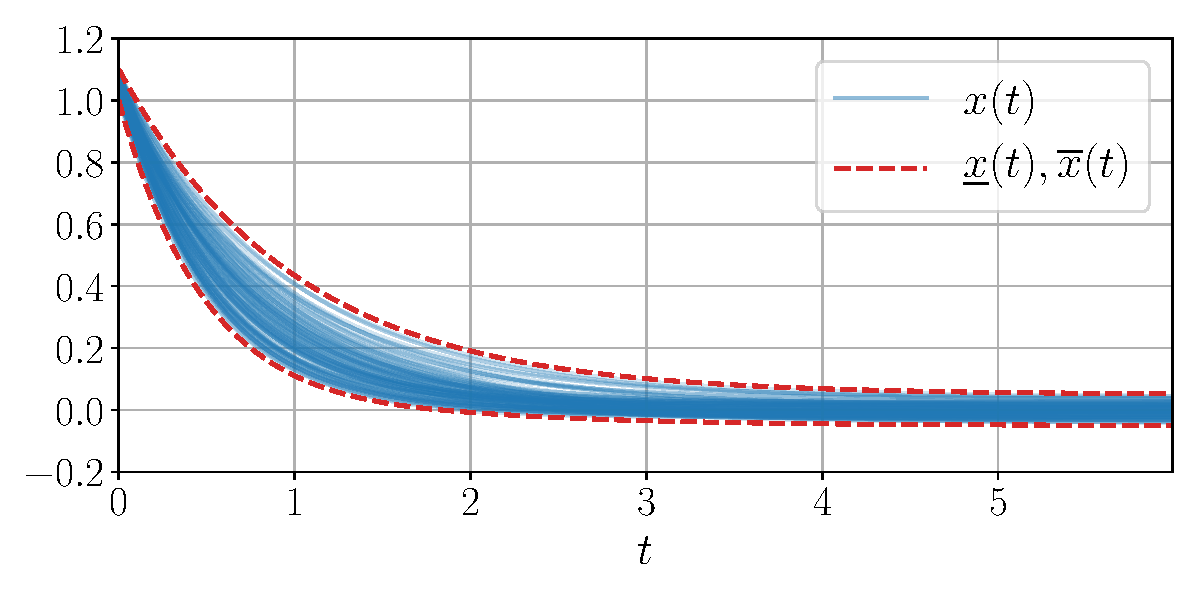
\includegraphics[width=0.8\linewidth]{img/predictor}
			\par\end{centering}
		\caption{\label{fig:IP_New} The results of prediction by \eqref{eq:interval-predictor}: the new predictor is stable and produces tight bounds.}
	\end{figure}
	Let us apply the predictor \eqref{eq:interval-predictor}
	to the motivating example:
	\begin{align*}
		\dot{\ux}(t) = {} & -\overline{\theta}\ux(t) - (\overline{\theta}-\underline{\theta})\ux^{-}(t) + \underline{\omega},\\
		\dot{\ox}(t) =  {} & -\overline{\theta}\ox(t) + (\overline{\theta}-\underline{\theta})\ox^{+}(t) + \overline{\omega},
	\end{align*}
	where $A_{0}=-\overline{\theta}$ is chosen, then $\Delta A_{+}=\overline{\theta}-\underline{\theta}$, $\Delta A_{-}=0$ and all conditions of \Cref{thm:interval-predictor-main} are verified. The results of simulation are shown in \Cref{fig:IP_New}. As we can see the new predictor generates very reasonable and bounded estimates. 
\end{example*}


\subsection{Frequency-based interval estimation}
\label{sec:Frequency}
The domain of convergence of the linear system \eqref{eq:linear-asympt}, and hence of \eqref{eq:interval-predictor}, can be tightened under an additional hypothesis that $\omega(t)$ has a known and bounded frequency spectrum.
Assume that there exist two signals $\underline{\omega},\overline{\omega}:\Real_{+}\to\Real^{r}$ and two vectors $\ux_{0},\ox_{0}\in\Real^{p}$ such that
\begin{gather*}
\underline{\omega}(t)\leq \omega(t)\leq\overline{\omega}(t),\quad\forall t\geq0,\\
\ux_{0}\leq x(0)\leq\ox_{0},
\end{gather*} and there is a matrix $L\in\Real^{p\times s}$ such that $A-LC$ is Hurwitz and Metzler, then an interval observer for the system \eqref{eq:LTI_syst} can be written as follows \citep{REZ11}:
\begin{align}
\label{eq:IO_LTI}
\begin{split}
\dot{\ux}(t) = {} & (A-LC)\ux(t)+Bu(t) +Ly(t)  +(D-LE)^{+}\underline{\omega}(t)-(D-LE)^{-}\overline{\omega}(t), \\
\dot{\ox}(t) = {} & (A-LC)\ox(t)+Bu(t) +Ly(t)  +(D-LE)^{+}\overline{\omega}(t)-(D-LE)^{-}\underline{\omega}(t), \\
 \text{with }\, & \ux(0)=\ux_{0},\;\ox(0)=\ox_{0}, 
\end{split}
\end{align}
guaranteeing the desired interval relations
\[
\ux(t)\leq x(t)\leq\ox(t),\quad\forall t\geq0.
\]
This solution uses only information about amplitude of the external input $\omega$, and its precision can be largely improved if we assume that there is also information about admissible frequency spectrum in $\omega$:
\begin{lemma}
	\label{lem:IntFreq}
	\begin{leftbar}[lemmabar]
	Let there exist $f_{1},f_{2}\in\Natural_{+}$ and $T,W>0$
	such that
	\[
	\omega(t)=a_{0}+\sum_{f=f_{1}}^{f_{2}}a_{f}\sin\left(\frac{2\pi f}{T}t+\phi_{s}\right),
	\]
	for some $a_{0},a_{f},\phi_{f}\in\Real$ with $f\in[f_{1},f_{2}]$ and $||d||\leq W$. Then for any $x(0)\in\Real^{n}$ in \eqref{eq:LTI_syst} and any $\epsilon>0$ there exists $\tau>0$ such that
	\[
	|x_{i}(t)|\leq\sup_{w\in[\frac{2\pi}{T}f_{1},\frac{2\pi}{T}f_{2}]}|e_{i}(jwI_{n}-A)^{-1}DE_{r}|W+\epsilon\quad\forall t\geq\tau,
	\]
	where $j$ corresponds to the imaginary unit, provided that the matrix $A$ is Hurwitz.
	\end{leftbar}
\end{lemma}
\begin{proof}
	The solution of the system \eqref{eq:LTI_syst} can be written as follows:
	\[
	x(t)=e^{At}x(0)+\int_{0}^{t}e^{A(t-\sigma)}(Bu(\sigma)+D\omega(\sigma))\dd\sigma,
	\]
	where the first term ($e^{At}x(0)$) is converging asymptotically to zero since the matrix $A$ is Hurwitz by hypothesis. And in order to estimate the second term, the Bode magnitude plot can be used, which provides the asymptotic amplitude of the state for the given frequency input. Under the introduced hypotheses, the frequency of the input lies in the interval $[\frac{2\pi}{T}f_{1},\frac{2\pi}{T}f_{2}]$ and the amplitude is upper-bounded by $W$, then there exist constants $\tau>0$ and $\epsilon>0$, related with $x(0)$, such that the claim of the lemma is true.
\end{proof}
The interval observer \eqref{eq:IO_LTI}, if we assume that $\overline{\omega}(t)=-\underline{\omega}(t)=WE_{r}$ and $L=0$, asymptotically will converge to the interval $[-|e_{i}A{}^{-1}BE_{r}|W,|e_{i}A{}^{-1}BE_{r}|W]$ (that corresponds to the result of \Cref{lem:IntFreq} with $f_{1}=f_{2}=0$), which is the estimate from Bode plot given for the frequency $0$, and it is a well-known fact that for many stable systems the Bode magnitude plot is a decreasing function of the frequency. Therefore, if the information about frequency spectrum is known and it is separated from zero, then the asymptotic interval accuracy can be significantly improved. Of course, \Cref{lem:IntFreq} can be applied iteratively for a decreasing sequence of $\epsilon>0$ and an increasing one in $\tau>0$.
\begin{example*}
	Let us illustrate these conclusions on a simple example:
	\begin{gather*}
	A=\left[\begin{array}{cc}
	-1 & 1\\
	0.1 & -1
	\end{array}\right],\;B=\left[\begin{array}{c}
	-2\\
	1
	\end{array}\right],\;L=0,\\
	\overline{\omega}(t)=-\underline{\omega}(t)=1,\\
	\ox_{0}=[2\;1]\tr,\;\ux_{0}=[-1\;-2]\tr.
	\end{gather*}
	And assume that
	$
	\omega(t)=d_0\sin(ft+\phi_0),\;f=7,
	$
	then the system trajectories and intervals are shown in \Cref{fig:IntFreq}. 
	\begin{figure}
		\begin{centering}
			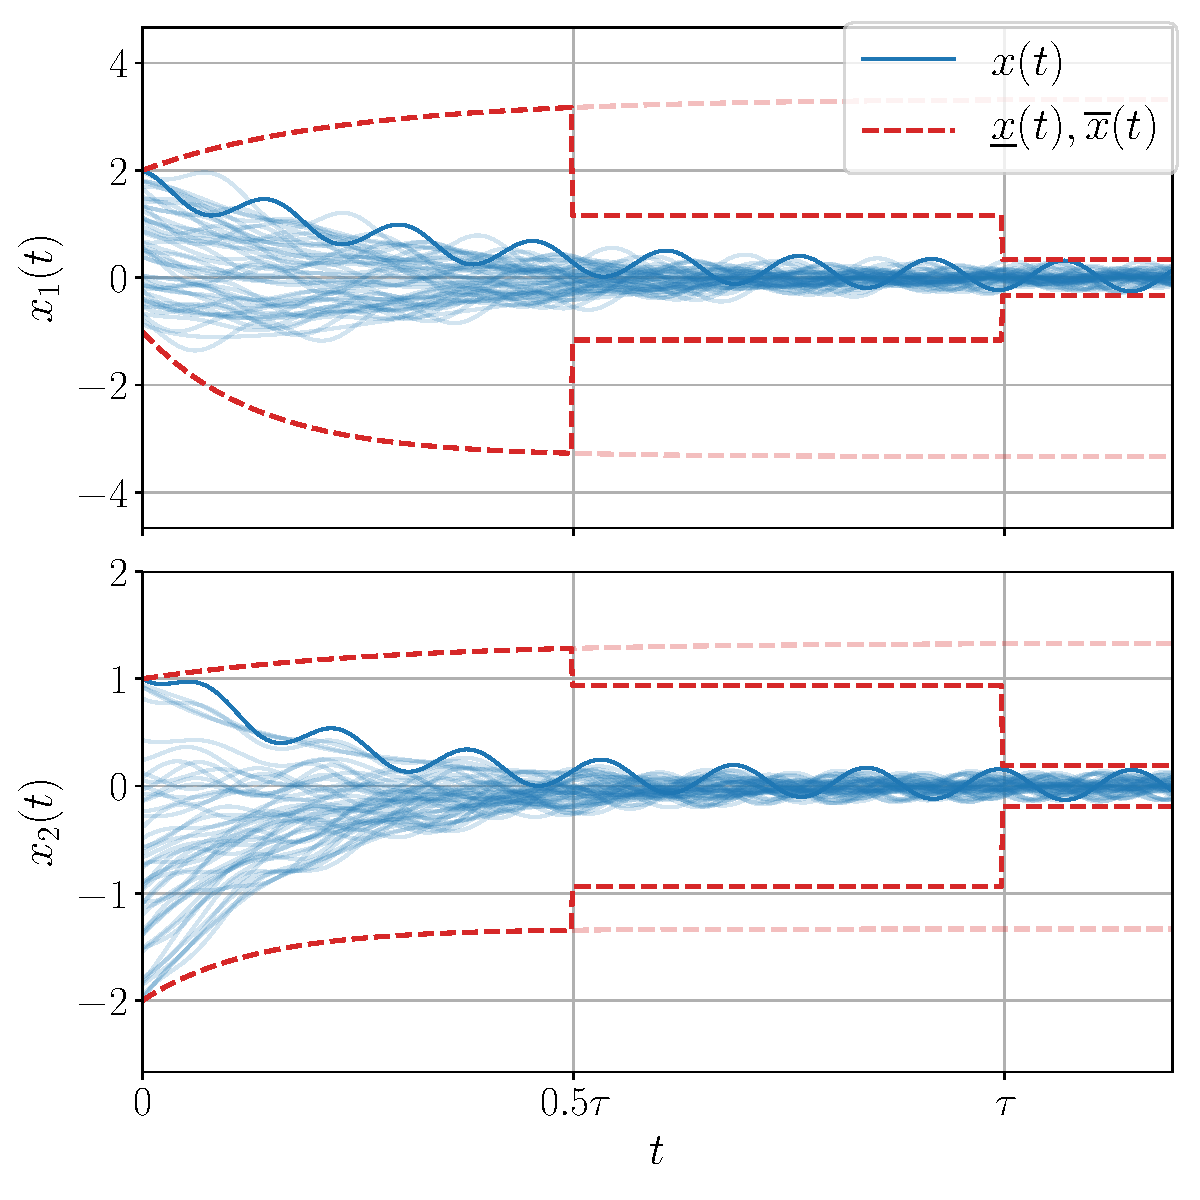
\includegraphics[width=0.8\linewidth]{img/asymptotic}
			\par\end{centering}
		\caption{\label{fig:IntFreq} The results of prediction for different values
			of the frequency. Taking $\tau=\frac{4}{\min_{i=\overline{1,n}}|\lambda_{i}(A)|}=5.85$ and $\epsilon=0.05,$ the trajectories of the interval observer \eqref{eq:IO_LTI} are presented for $t\leq0.5\tau$, and as we can conclude, these estimates are rather conservative. Next, for $t\in[0.5\tau,\tau]$ the estimates given in \Cref{lem:IntFreq} for the case $s_{1}=s_{2}=0$ are shown, which are already more accurate. Finally, for $t\geq\tau$ the estimates of \Cref{lem:IntFreq} are presented for $s_{1}=s_{2}=s$, which demonstrate a definite improvement. }
	\end{figure}
\end{example*}

\subsection{Prediction for a self-driving vehicle}
\label{sec:interval-prediction-experiments}
We consider the problem of safe decision-making for autonomous highway driving \citep{highway-env}\footnote{Videos and source code of all experiments are available at \href{https://eleurent.github.io/interval-prediction/}{https://eleurent.github.io/interval-prediction/}.}.

As described in \Cref{chapter:3}, an autonomous vehicle is driving on a highway populated with $N$ other agents, and uses \glsxtrlong{MPC} to plan a sequence of decisions. To that end, it relies on parametrized dynamical model for each agent to predict the future trajectory of each traffic participant: $$\dot{x}_i=f_i(x,\theta_i),\;i\in[N_v],$$ where $f_i$ are described in \Cref{chapter:3}, $x_i\in\Real^4$ is the state of a vehicle, $x = [x_1^\top,\dots,{x_{N_v}}^\top]^\top\in\Real^{4N_v}$ and $\theta_i\in\Real^5$ is the corresponding vector of unknown parameters. Crucially, this system describes the couplings and interactions between vehicles, so that the autonomous agent can properly anticipate their reactions. 
However, we assume that we do not have access to the true values of the behavioural parameters $\theta=[\theta_1,\dots,\theta_{N_v}]^\top$; instead, we merely know that these parameters lie in a set of admissible values $\Theta\subset\Real^{5N_v}$. In order to act safely in the face of uncertainty, the agent must consider all possible vehicle trajectories in order to take its decisions. In this section, we focus on how to compute these trajectory enclosures through interval prediction.

\subsubsection{\gls{LPV} formulation}

The system presented in \Cref{chapter:3} is non-linear and must be cast into the \gls{LPV} form. We approximate the non-linearities induced by the trigonometric operators through equilibrium linearisation around $y_i=y_{L_i}$ and $\psi_i=\psi_{L_i}$.

This yields the following longitudinal dynamics:
\begin{align*}
\dot{p}^x_i &= v_i,\\
\dot v_i &= \theta_{i,1} (v_0 - v_i) + \theta_{i,2} (v_{f_i} - v_i) + \theta_{i,3}(p^x_{f_i} - p^x_i - d_0 - v_i T),
\end{align*}
where $\theta_{i,2}$ and $\theta_{i,3}$ are set to $0$ whenever the corresponding features are not active.

It can be rewritten in the form $$\dot{x} = \structureddynamics(x-x_c) + d.$$ For example, in the case of two vehicles only,
\begin{equation*}
x = \begin{bmatrix}
p^x_i \\
p^x_{f_i} \\
v_i \\
v_{f_i} \\
\end{bmatrix}
,\quad
x_c = \begin{bmatrix}
-d_0-v_0 T \\
0 \\
v_0\\
v_0 \\
\end{bmatrix}
,\quad
d = \begin{bmatrix}
v_0 \\
v_0 \\
0\\
0\\
\end{bmatrix}
\end{equation*}

\begin{equation*}
\structureddynamics
=
\begin{blockarray}{ccccc}
& i & f_i & i & f_i \\
\begin{block}{c[cccc]}
i & 0 & 0 & 1 & 0 \\
f_i & 0 & 0 & 0 & 1 \\
i & -\theta_{i,3} & \theta_{i,3} & -\theta_{i,1}-\theta_{i,2}-\theta_{i,3} & \theta_{i,2} \\
f_i & 0 & 0 & 0 & -\theta_{f_i,1} \\
\end{block}
\end{blockarray}
\end{equation*}

The lateral dynamics are in a similar form:
\begin{equation*}
\begin{bmatrix}
\dot{p}^y_i \\
\dot{\psi}_i \\
\end{bmatrix}
=
\begin{bmatrix}
0 & v_i \\
-\frac{\theta_{i,4} \theta_{i,5}}{v_i} & -\theta_{i,5}
\end{bmatrix}
\begin{bmatrix}
p^y_i - p^y_{L_i} \\
\psi_i - \psi_{L_i}
\end{bmatrix}
+
\begin{bmatrix}
v_i\psi_{L_i} \\
0
\end{bmatrix}
\end{equation*}
Here, the dependency in $v_i$ is seen as an uncertain parametric dependency, \ie $\theta_{i,6}=v_i$, with constant bounds assumed for $v_i$ using an overset of the longitudinal interval predictor.

\subsubsection{Change of coordinates}
In both cases, the obtained polytope centre $A_0$ is non-Metzler.
We use \Cref{lem:l2,lem:l3} to compute a similarity transformation of coordinates. Precisely, we ensure that the polytope is chosen so that its centre $A_0$ is diagonalisable having real eigenvalues, and perform an eigendecomposition to compute its change of basis matrix $S$. The transformed system $x'=S^{-1}(x-x_c)$ verifies \Cref{assumpt:polytope} as required to apply the interval predictor of \Cref{thm:interval-predictor-main}. Finally, the obtained predictor is transformed back to the original coordinates $x$ by using the interval arithmetic of \Cref{lem:interval}.

\subsubsection{Results}

\begin{figure}
	\begin{center}
	\begin{subfigure}[b]{0.75\linewidth}
		\centering
		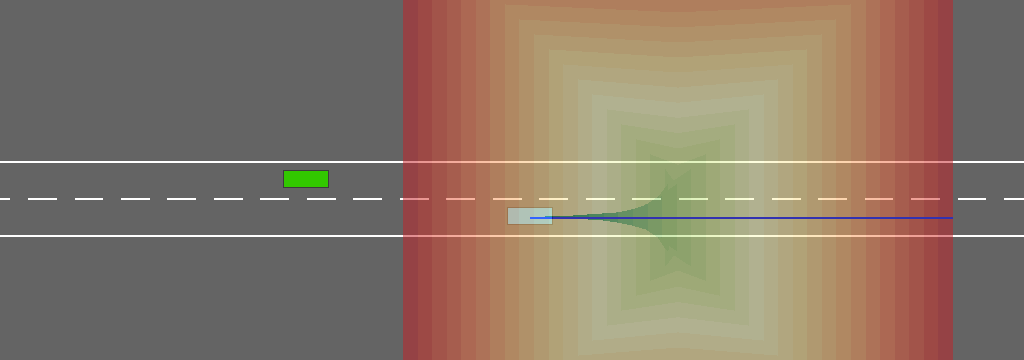
\includegraphics[width=\textwidth]{img/driving_observer.png}
		\caption{The naive predictor \eqref{eq:predictor-naive} quickly diverges}
		\label{sub:hw-a}
	\end{subfigure}
	\begin{subfigure}[b]{0.75\linewidth}
		\centering
		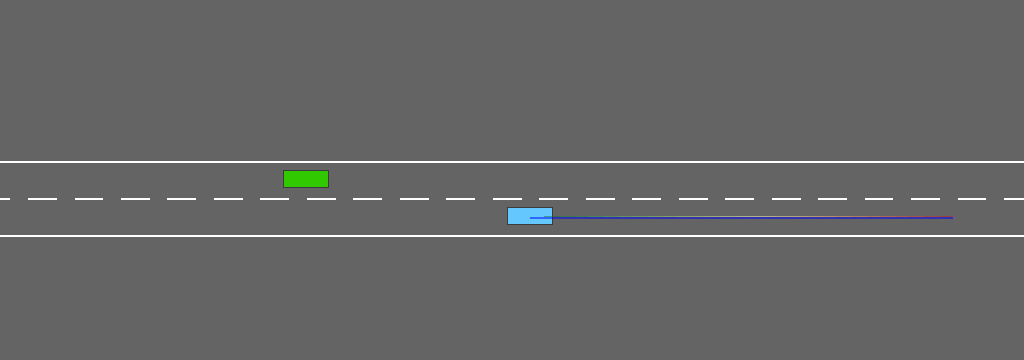
\includegraphics[width=\textwidth]{img/driving_predictor.png}
		\caption{The proposed predictor \eqref{eq:interval-predictor} remains stable}
		\label{sub:hw-b}
	\end{subfigure}
	\begin{subfigure}[b]{0.75\linewidth}
		\centering
		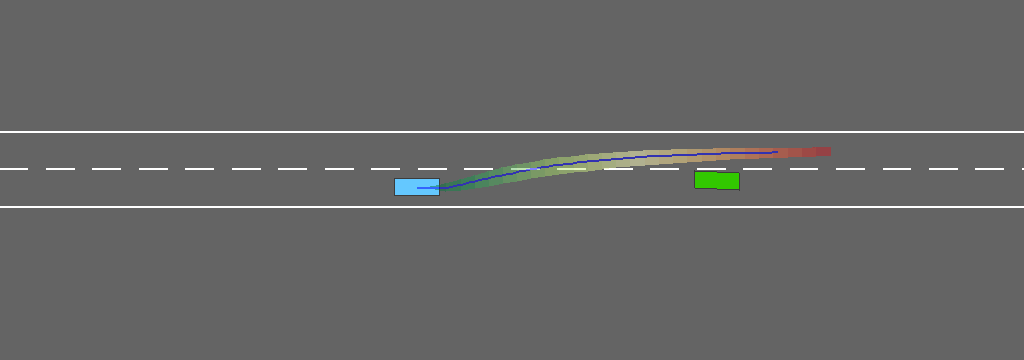
\includegraphics[width=\textwidth]{img/lane_change_predictor.png}
		\caption{Prediction during a lane change manoeuvre}
		\label{sub:hw-c}
	\end{subfigure}
	\begin{subfigure}[b]{0.75\linewidth}
		\centering
		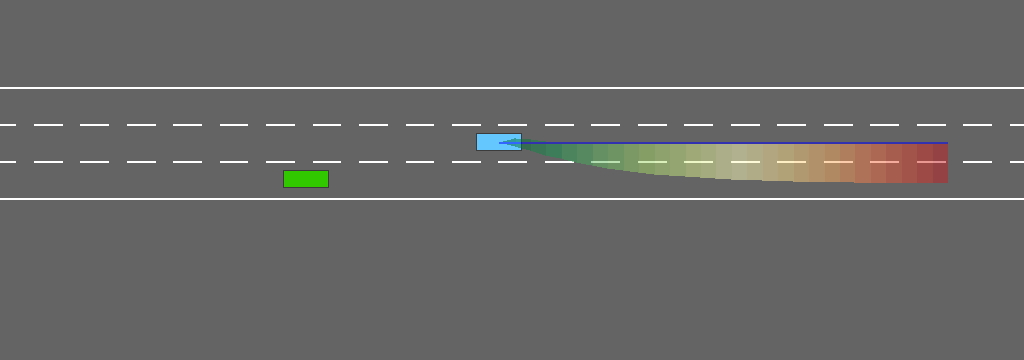
\includegraphics[width=\textwidth]{img/overtake.png}
		\caption{Prediction with uncertainty in the followed lane $L_i$}
		\label{sub:hw-d}
	\end{subfigure}
	\end{center}
	\caption{State intervals obtained by the two methods in different conditions.}
	\label{fig:highway}
\end{figure}


We show the resulting intervals in \Cref{fig:highway}. The target vehicle with uncertain behaviour is in blue, while the ego-vehicle is in green. Its trajectory interval is computed over a duration of two seconds and represented by an area filled with a colour gradient representing time. The ground-truth trajectory is shown in blue. In \Cref{sub:hw-a}, we observe that the direct predictor \eqref{eq:predictor-naive} is unstable and quickly diverges to cover the whole road, thus hindering any sensible decision-making. In prior work \citep{Leurent2018approximate}, we had to circumvent this issue by subdividing $\Theta$ and $[\ux, \ox]$ to reduce the initial overestimations and merely delay the divergence \citep{Adrot2003}, at the price of a heavy computational load. In stark contrast, we see in \Cref{sub:hw-b} that the novel predictor \eqref{eq:interval-predictor} is very stable even over long horizons, which allows the ego-vehicle to plan an overtaking manoeuvre. Until then, there was little uncertainty in the predicted trajectory for the target vehicle was isolated, but as the ego-vehicle cuts into its lane in \Cref{sub:hw-c}, we start seeing the effects of uncertain interactions between the two vehicles, in both longitudinal and lateral directions. Note that this formulation naturally exhibits socially aware predictions, and accounts for these interactions. Our framework is also quite flexible in representing different assumptions on the admissible behaviours. For instance, we show in \Cref{sub:hw-d} a simulation in which we model right-hand traffic where drivers are expected to keep to the rightmost lane. In such a situation, it is reasonable to assume that in the absence of any obstacle in front, a vehicle driving on the middle lane will either stay there or return to the right lane, but has no incentive to change to the left lane. This simple assumption on $L_i$ can easily be incorporated in the interval predictor, and enables the emergence of a realistic behaviour when running the robust decision-making procedure: the ego-vehicle cannot pass another vehicle by its right side, and can only overtake it by its left side. These behaviours displaying safe reasoning under uncertainty are showcased in the attached videos.

\subsection*{Section conclusion}

The prediction problem for uncertain \gls{LPV} systems is solved by designing an interval predictor, which is described by nonlinear differential equations, and whose stability is evaluated using a new Lyapunov function. The corresponding robust stability conditions are expressed in terms of \glspl{LMI}. An approach is presented to improve the asymptotic accuracy of interval estimation or prediction in \gls{LTI} systems provided that the exogenous inputs have a known spectrum of frequencies. The proficiency of the methods is demonstrated in application to a problem of safe motion planning for a self-driving car.



\section{Robust stabilisation and constraint satisfaction}
\label{sec:robust-stabilisation}

In this section, as a first application of the estimation and prediction tools introduced above, we set out to design a robust control $u(t)$ that stabilises \eqref{eq:dynamics}, \eqref{eq:outputs} at a vicinity of the origin under \Cref{assumpt:structure,assumpt:bounded-state,assumpt:bounded-noise}
such that
\begin{equation}
x(t)\in\safestates,\;u(t)\in\safecontrols\quad\forall t\geq0,\tag{\ref{eq:constraints}}
\end{equation}
where $[\ux_{0},\ox_{0}]\subset\safestates\subset\Real^{p}$ and $\safecontrols\subset\Real^{q}$ are given bounded constraint sets for the state and the control, respectively.

\subsection{Stabilising control for \eqref{eq:predictor-naive} and \eqref{eq:interval-predictor}}

Note that both interval predictors, \eqref{eq:predictor-naive} and
\eqref{eq:interval-predictor}, admit a representation in the form
\begin{equation}
\dot{\xi}(t)=\cA_{0}\xi(t)+\cA_{1}\xi^{+}(t)+\cA_{2}\xi^{-}(t)+\cB u(t)+\confidence(t),\label{eq:predictor}
\end{equation}
where $\xi(t)=[\ux^{\top}(t)\;\ox^{\top}(t)]^{\top}\in\Real^{2p}$
is the extended state vector of the predictors,
\[
\confidence(t)=\left[\begin{array}{cc}
D^{+} & -D^{-}\\
-D^{-} & D^{+}
\end{array}\right]\left[\begin{array}{c}
\underline{\omega}(t)\\
\overline{\omega}(t)
\end{array}\right]\in\Real^{2p}
\]
is the external known input, $\cB=[B^{\top}\;B^{\top}]^{\top}$, 
\[
\cA_{0}=\left[\begin{array}{cc}
0 & 0\\
0 & 0
\end{array}\right],\;\cA_{1}=\left[\begin{array}{cc}
\underline{A}^{+} & -\underline{A}^{-}\\
-\overline{A}^{-} & \overline{A}^{+}
\end{array}\right],\;\cA_{2}=\left[\begin{array}{cc}
-\overline{A}^{+} & \overline{A}^{-}\\
\underline{A}^{-} & -\underline{A}^{+}
\end{array}\right]
\quad \text{for \eqref{eq:predictor-naive},}
\]
 and
\[
\cA_{0}=\left[\begin{array}{cc}
A_{0} & 0\\
0 & A_{0}
\end{array}\right],\;\cA_{1}=\left[\begin{array}{cc}
0 & -\Delta A_{-}\\
0 & \Delta A_{+}
\end{array}\right],\;\cA_{2}=\left[\begin{array}{cc}
-\Delta A_{+} & 0\\
\Delta A_{-} & 0
\end{array}\right]
\quad \text{for \eqref{eq:interval-predictor}.}
\]
Note that \eqref{eq:predictor} is a nonlinear system due to the presence of globally Lipschitz nonlinearities $\xi^{+}(t)$ and $\xi^{-}(t)$. 

Due to the inclusion property \eqref{eq:inclusion-property}, the boundedness of $\xi(t)$
implies the same property of $x(t)$. Therefore, in order to regulate
\eqref{eq:dynamics} it is required to design a state feedback $u(t)$
minimizing the asymptotic amplitude of the state $\xi(t)$ for given
input $\confidence(t)$ \citep{Efimov_tac2013}. In other words, it is necessary
to design a control $u(t)$ that input-to-state stabilises \eqref{eq:predictor}.
It is proposed to look for such a control in the form
\begin{equation}
u(t)=K_{0}\xi(t)+K_{1}\xi^{+}(t)+K_{2}\xi^{-}(t)+S\confidence(t),\label{eq:control_pr}
\end{equation}
where $K_{0},K_{1},K_{2}\in\Real^{q\times2p}$ and $S\in\Real^{q\times2p}$
are the gains to be designed (\eqref{eq:control_pr} contains a nonlinear
feedback). The selection of $S$ is simple, it has to minimise the
norm of $\cB S+I_{2p}$, and it can be made independently of $K_{0},K_{1},K_{2}$.
Therefore, denoting $\tilde{\confidence}(t)=(\cB S+I_{2p})\confidence(t)$ the
closed-loop system \eqref{eq:predictor}, \eqref{eq:control_pr} takes
the form:
\begin{equation}
\dot{\xi}(t)=\cD_{0}\xi(t)+\cD_{1}\xi^{+}(t)+\cD_{2}\xi^{-}(t)+\tilde{\confidence}(t),\label{eq:closed-loop_pr}
\end{equation}
where $\cD_{i}=\cA_{i}+\cB K_{i}$ for $i\in[3]$, and the restrictions,
which the gains $K_{0},K_{1},K_{2}$ have to respect, are given below:
\begin{theorem}
	\begin{leftbar}[theorembar]
	\label{thm:ISS_pr} If there exist diagonal matrices $P$, $Q$, $Q_{+}$,
	$Q_{-}$, $Z_{+}$, $Z_{-}$, $\Psi_{+}$, $\Psi_{-}$, $\Psi$, $\Gamma\in\Real^{2p\times2p}$
	such that the following linear matrix inequalities are satisfied:
	\begin{gather*}
	P+\min\{Z_{+},Z_{-}\}>0,\;\Upsilon\preceq0,\;\Gamma>0,\\
	Q+\min\{Q_{+},Q_{-}\}+2\min\{\Psi_{+},\Psi_{-}\}>0,
	\end{gather*}
	where
	\begin{gather*}
	\Upsilon=\left[\begin{array}{cccc}
	\Upsilon_{11} & \Upsilon_{12} & \Upsilon_{13} & P\\
	\Upsilon_{12}^{\top} & \Upsilon_{22} & \Upsilon_{23} & Z_{+}\\
	\Upsilon_{13}^{\top} & \Upsilon_{23}^{\top} & \Upsilon_{33} & -Z_{-}\\
	P & Z_{+} & -Z_{-} & -\Gamma
	\end{array}\right],\\
	\Upsilon_{11}=\cD_{0}^{\top}P+P\cD_{0}+Q,\;\Upsilon_{12}=\cD_{0}^{\top}Z_{+}+P\cD_{1}+\Psi_{+},\\
	\Upsilon_{13}=P\cD_{2}-\cD_{0}^{\top}Z_{-}-\Psi_{-},\;\Upsilon_{22}=Z_{+}\cD_{1}+\cD_{1}^{\top}Z_{+}+Q_{+},\\
	\Upsilon_{23}=Z_{+}\cD_{2}-\cD_{1}^{\top}Z_{-}+\Psi,\;\Upsilon_{33}=-Z_{-}\cD_{2}-\cD_{2}^{\top}Z_{-}+Q_{-},
	\end{gather*}
	then \eqref{eq:closed-loop_pr} is input-to-state stable with respect
	to $\underline{\omega},\overline{\omega}$.
	\end{leftbar}
\end{theorem}
Note that the requirement that the matrix $P$ has to be diagonal is not
restrictive, since for a Metzler matrix $\cD_{0}$ (the case of \eqref{eq:predictor-naive}
and \eqref{eq:interval-predictor}), its stability is equivalent to
existence of a diagonal solution $P$ of the Lyapunov equation $\cD_{0}^{\top}P+P\cD_{0}\prec0$
\citep{FarinaRinaldi2000}.
\begin{proof}
	Consider a candidate Lyapunov function
	\begin{gather*}
	V(\xi)=\xi^{\top}P\xi+\xi{}^{\top}Z_{+}\xi^{+}-\xi^{\top}Z_{-}\xi^{-}\\
	=\sum_{k=1}^{2p}P_{k,k}\xi_{k}^{2}+(Z_{+})_{k,k}\xi_{k}\xi_{k}^{+}-(Z_{-})_{k,k}\xi_{k}\xi_{k}^{-}\\
	=\sum_{k=1}^{2p}P_{k,k}\xi_{k}^{2}+(Z_{+})_{k,k}|\xi_{k}|\xi_{k}^{+}+(Z_{-})_{k,k}|\xi_{k}|\xi_{k}^{-},
	\end{gather*}
	which is positive definite provided that
	\[
	P+\min\{Z_{+},Z_{-}\}>0
	\]
	since all terms in $V$ are quadratic-like, and whose derivative for
	the system \eqref{eq:closed-loop_pr} dynamics takes the form
	\begin{gather*}
	\dot{V}=2\dot{\xi}^{\top}P\xi+2\dot{\xi}^{\top}Z_{+}\xi^{+}-2\dot{\xi}^{\top}Z_{-}\xi^{-}\\
	=\left[\begin{array}{c}
	\xi\\
	\xi^{+}\\
	\xi^{-}\\
	\tilde{\confidence}
	\end{array}\right]^{\top}\Upsilon\left[\begin{array}{c}
	\xi\\
	\xi^{+}\\
	\xi^{-}\\
	\tilde{\confidence}
	\end{array}\right]-\xi^{\top}Q\xi-(\xi^{+})^{\top}Q_{+}\xi^{+}\\
	-(\xi^{-})^{\top}Q_{-}\xi^{-}-2(\xi^{+})^{\top}\Psi\xi^{-}-2(\xi^{+})^{\top}\Psi_{+}\xi\\
	-2(-\xi^{-})^{\top}\Psi_{-}\xi+\tilde{\confidence}^{\top}\Gamma\tilde{\confidence}.
	\end{gather*}
	Note that
	\begin{gather*}
	(\xi^{+})^{\top}\Psi\xi^{-}=0,\\
	(\xi^{+})^{\top}\Psi_{+}\xi\geq0,\;(-\xi^{-})^{\top}\Psi_{-}\xi\geq0
	\end{gather*}
	for any diagonal matrix $\Psi$ and $\Psi_{+}\geq0$, $\Psi_{-}\geq0$.
	Hence, if $\Upsilon\preceq0$, as it is assumed in the theorem, we
	obtain that
	\begin{align*}
		\dot{V}  \leq {} & -\xi^{\top}Q\xi-(\xi^{+})^{\top}Q_{+}\xi^{+}-(\xi^{-})^{\top}Q_{-}\xi^{-}\\
		 & -2(\xi^{+})^{\top}\Psi_{+}\xi-2(-\xi^{-})^{\top}\Psi_{-}\xi+\tilde{\confidence}^{\top}\Gamma\tilde{\confidence}\\
		 \leq {} & -\xi^{\top}\Omega\xi+\tilde{\confidence}^{\top}\Gamma\tilde{\confidence},
	\end{align*}
	where
	\[
	\Omega=Q+\min\{Q_{+},Q_{-}\}+2\min\{\Psi_{+},\Psi_{-}\}>0,
	\]
	is a diagonal matrix. The substantiated properties of $V$ and its
	derivative imply that \eqref{eq:closed-loop_pr} is input-to-state
	stable \citep{Sontag:01:Springer,Dashkovskiy:11:AiT} with respect
	to the input $\tilde{\confidence}$ (or, by its definition, with respect
	to $(\underline{\omega},\overline{\omega})$).
\end{proof}
Following the proof of \Cref{thm:ISS_pr}, for all $\xi\in\Real^{2p}$,
\[
\xi^{\top}(P+\min\{Z_{+},Z_{-}\})\xi\leq V(\xi)\leq\xi^{\top}(P+Z_{+}^{+}+Z_{-}^{+})\xi,
\]
then
\[
\dot{V}\leq-\alpha V+\tilde{\confidence}^{\top}\Gamma\tilde{\confidence}
\]
for all $\xi,\tilde{\confidence}\in\Real^{2p}$, where
\[
\alpha=\min_{i\in[2p]}\lambda_{i}\left(\Omega(P+Z_{+}^{+}+Z_{-}^{+})^{-1}\right),
\]
and we can define the set (recall that the signal $\tilde{\confidence}(t)$
is known for all $t\geq0$)
\begin{equation}
\safestates_{f}=\{\xi\in\Real^{2p}:V(\xi)\leq\alpha^{-1}\sup_{t\geq0}|\tilde{\confidence}^{\top}(t)\Gamma\tilde{\confidence}(t)|\},\label{eq:X_f}
\end{equation}
as the set that asymptotically attracts all trajectories in \eqref{eq:closed-loop_pr}.

The conditions of \Cref{thm:ISS_pr} assume that the control
gains $K_{0},K_{1},K_{2}$ are given, let us find these gains as solutions
of linear matrix inequalities:
\begin{corollary}
	\begin{leftbar}[corollarybar]
	If there exist diagonal matrices $P$, $\tilde{Q}$, $\tilde{Q}_{+}$,
	$\tilde{Q}_{-}$, $Z_{+}$, $Z_{-}$, $\tilde{\Psi}_{+}$, $\tilde{\Psi}_{-}$,
	$\tilde{\Psi}$, $\Gamma\in\Real^{2p\times2p}$ and matrices $U_{0},U_{1},U_{2}\in\Real^{q\times2p}$
	such that the following linear matrix inequalities are satisfied:
	\begin{gather*}
	P>0,\;Z_{+}>0,\;Z_{-}>0,\;\Pi\preceq0,\;\Gamma>0,\\
	\tilde{Q}+\min\{\tilde{Q}_{+},\tilde{Q}_{-}\}+2\min\{\tilde{\Psi}_{+},\tilde{\Psi}_{-}\}>0,
	\end{gather*}
	where
	\begin{gather*}
	\Pi=\left[\begin{array}{cccc}
	\Pi_{11} & \Pi_{12} & \Pi_{13} & I\\
	\Pi_{12}^{\top} & \Pi_{22} & \Pi_{23} & I\\
	\Pi_{13}^{\top} & \Pi_{23}^{\top} & \Pi_{33} & -I\\
	I & I & -I & -\Gamma
	\end{array}\right],\\
	\Pi_{11}=P^{-1}\cA_{0}^{\top}+\cA_{0}P^{-1}+U_{0}^{\top}\cB^{\top}+\cB U_{0}+\tilde{Q},\\
	\Pi_{12}=\cA_{1}Z_{+}^{-1}+\cB U_{1}+P^{-1}\cA_{0}^{\top}+U_{0}^{\top}\cB^{\top}+\tilde{\Psi}_{+},\\
	\Pi_{13}=\cA_{2}Z_{-}^{-1}+\cB U_{2}-P^{-1}\cA_{0}^{\top}-U_{0}^{\top}\cB^{\top}-\tilde{\Psi}_{-},\\
	\Pi_{22}=Z_{+}^{-1}\cA_{1}^{\top}+\cA_{1}Z_{+}^{-1}+U_{1}^{\top}\cB^{\top}+\cB U_{1}+\tilde{Q}_{+},\\
	\Pi_{23}=\cA_{2}Z_{-}^{-1}+\cB U_{2}-Z_{+}^{-1}\cA_{1}^{\top}-U_{1}^{\top}\cB^{\top}+\tilde{\Psi},\\
	\Pi_{33}=\tilde{Q}_{-}-Z_{-}^{-1}\cA_{2}^{\top}-\cA_{2}Z_{-}^{-1}-U_{2}^{\top}\cB^{\top}-\cB U_{2},
	\end{gather*}
	then \eqref{eq:closed-loop_pr} for $K_{0}=U_{0}P$, $K_{1}=U_{1}Z_{+}$
	and $K_{2}=U_{2}Z_{-}$ is input-to-state stable with respect to the
	inputs $\underline{\omega},\overline{\omega}$.
	\end{leftbar}
\end{corollary}
\begin{proof}
	Note that the conditions $P>0$, $Z_{+}>0$, $Z_{-}>0$ imply $P+\min\{Z_{+},Z_{-}\}>0$,
	and 
	\[
	\Upsilon=\left[\begin{array}{cccc}
	P & 0 & 0 & 0\\
	0 & Z_{+} & 0 & 0\\
	0 & 0 & Z_{-} & 0\\
	0 & 0 & 0 & I_{2p}
	\end{array}\right]\Pi\left[\begin{array}{cccc}
	P & 0 & 0 & 0\\
	0 & Z_{+} & 0 & 0\\
	0 & 0 & Z_{-} & 0\\
	0 & 0 & 0 & I_{2p}
	\end{array}\right]
	\]
	under substitution $U_{0}=K_{0}P^{-1}$, $U_{1}=K_{1}Z_{+}^{-1}$,
	$U_{2}=K_{2}Z_{-}^{-1}$, $\tilde{Q}=P^{-1}QP^{-1}$, $\tilde{Q}_{+}=Z_{+}^{-1}Q_{+}Z_{+}^{-1}$,
	$\tilde{Q}_{-}=Z_{-}^{-1}Q_{-}Z_{-}^{-1}$, $\tilde{\Psi}=Z_{-}^{-1}\Psi Z_{+}^{-1}$,
	$\tilde{\Psi}_{+}=P^{-1}\Psi_{+}Z_{+}^{-1}$ and $\tilde{\Psi}_{-}=P^{-1}\Psi_{-}Z_{-}^{-1}$.
	Hence, $\Upsilon\preceq0$ provided that $\Pi\preceq0$. The inequalities
	$\tilde{Q}+\min\{\tilde{Q}_{+},\tilde{Q}_{-}\}+2\min\{\tilde{\Psi}_{+},\tilde{\Psi}_{-}\}>0$
	and $Q+\min\{Q_{+},Q_{-}\}+2\min\{\Psi_{+},\Psi_{-}\}>0$ are equivalent
	due to the diagonal structure of all matrices. Therefore, under introduced
	restrictions all conditions of \Cref{thm:ISS_pr} are verified
	for $K_{0}=U_{0}P$, $K_{1}=U_{1}Z_{+}$ and $K_{2}=U_{2}Z_{-}$.
\end{proof}
The requirements imposed on $P,Z_{+},Z_{-}$ in this corollary are
more restrictive than the conditions of \Cref{thm:ISS_pr},
but it allows the gains $K_{0},K_{1},K_{2}$ to be efficiently calculated.

Under conditions of \Cref{thm:ISS_pr}, the control \eqref{eq:control_pr} ensures stabilisation of the predictor \eqref{eq:predictor} (\ie \eqref{eq:predictor-naive} or \eqref{eq:interval-predictor}) in a vicinity $\safestates_{f}$ of the origin. The size of the vicinity is proportional to the system \eqref{eq:dynamics} uncertainty (it can be optimized by the choice of $K_{0},K_{1},K_{2}$), and due to \eqref{eq:inclusion-property}, it implies that the system \eqref{eq:dynamics} also will reach a neighbourhood of the origin under the control \eqref{eq:control_pr}. Hence, the posed control problem would be solved provided that \eqref{eq:constraints} holds. In order to ensure the robust constraint satisfaction we consider an \gls{MPC} design in the next section.

\subsection{Robust constraint satisfaction}
\label{sec:stab-robust-control}

For brevity, the results of this section are given for the predictor
\eqref{eq:interval-predictor} only (and the case of \eqref{eq:predictor-naive}
can be considered by skipping \Cref{assumpt:metzler} in the
formulation). We need the following hypothesis in this section:
\begin{assumption}
	\begin{leftbar}[assumptionbar]
	\label{assumpt:feasible-constr} There exist $K_{0},K_{1},K_{2}\in\Real^{q\times2p}$	satisfying the conditions of \Cref{thm:ISS_pr} for the matrices $A_{0}$ and $\Delta A_{i}$ with $i\in[M]$ calculated in \eqref{eq:polytope}	for $\confidenceset=\Theta$, and
	\[
	\safestates_{f}\subset\safestates^{2},
	\]
	where the corresponding set $\safestates_{f}$ is given in \eqref{eq:X_f}, and
	\[
	K_{0}\xi+K_{1}\xi^{+}+K_{2}\xi^{-}+S\confidence(t)\in\safecontrols
	\]
	for any $\xi\in\safestates_{f}$ and $t\geq0$.
	\end{leftbar}
\end{assumption}
These properties guarantee that there exists a control \eqref{eq:control_pr} that can be always applied to stabilise the predictor \eqref{eq:interval-predictor}
(the worst-case estimate set $\Theta$ is used to calculate the system matrices) and into the set $\safestates_{f}$ the restrictions \eqref{eq:constraints} also hold for such a control. Recall that we denote $\timestep>0$ the time step and $t_{n}=n\timestep$ for $n\in\Natural_{+}$, and define $T>\timestep $ as the \gls{MPC} prediction horizon, \ie at each $t_n\geq0$, to design
the input $u(t)$, an optimal control problem is solved on the interval $[t_n,t_n+T]$, and this optimal control problem is resolved again after $\timestep$ units of time (on the interval $[t_n,t_{n+1} = t_n+\timestep)$ the obtained
optimal control is applied). Then the developed \gls{MPC} algorithm can be formalized as follows for
any $t_{n}\geq0$:

\begin{enumerate}
	\item Take the confidence region $\confidenceset$ from \eqref{eq:confidence-ellipsoid} and calculate the matrices $A_{0}$ and $\Delta A_{i}$ with $i\in[2^d]$ for \eqref{eq:polytope}.
	\item Find
	\begin{equation}
	\label{eq:OCP}
	\cU=\argmin_{u:[t_{n},t_{n}+T]\to\Real^{q}}\xi(t_{n}+T)^{\top}W_{1}\xi(t_{n}+T)
	+\int_{t_{n}}^{t_{n}+T}\xi^{\top}(s)W_{2}\xi(s)+u(s)^{\top}W_{3}u(s)\dd s, 
	\end{equation}
	where $W_{i}\in\Real^{2p\times2p}$ are given positive definite symmetric
	matrices, such that the following constraints are satisfied: 
	\begin{enumerate}
		\item $\xi:[t_{n},t_{n}+T]\to\Real^{2p}$ is a solution of \eqref{eq:interval-predictor}
		with $t=t_{n}$.
		\item $\xi(s)\in\safestates^{2}$ and $u(s)\in\safecontrols$ for $s\in[t_{n},t_{n}+T]$; 
		\item $\xi(t_{n}+T)\in\safestates_{f}$.
	\end{enumerate}
	\item For $t\in[t_{n},t_{n+1})$ select
	\begin{equation}
	u(t)=\begin{cases}
	\cU(t) & \xi(t_{n})\notin\safestates_{f}\\
	\eqref{eq:control_pr} & \xi(t_{n})\in\safestates_{f}
	\end{cases},\label{eq:control}
	\end{equation}
	where $K_{0},K_{1},K_{2}$ are taken from \Cref{assumpt:feasible-constr}.
\end{enumerate}
As we can conclude, the idea of the proposed dual \gls{MPC} scheme \citep[see also][]{Michalska1993,Mayne2000,Mayne2009} is to use an open-loop optimal control to reach a neighbourhood of the origin $\safestates_{f}$ ensuring a robust constraint satisfaction \eqref{eq:constraints}, where a closed-loop control \eqref{eq:control_pr} can be applied, which provides asymptotic performances (stability and robustness, also with constraint satisfaction due to \Cref{assumpt:feasible-constr} and the definition of the terminal set \eqref{eq:X_f}). 

%The proposed rule of the initial condition setup for prediction \eqref{eq:update} is chosen in a way to use all available information about the state: at $t_{0}=0$ it is intersection of the measured interval $[y_{1}(t_{n})-\underline{\nu}_{1}(t_{n}),y_{1}(t_{n})+\overline{\nu}_{1}(t_{n})]$ and the set $[\ux_{0},\ox_{0}]$ (since we assume that initially the state is in this set by  \Cref{assumpt:bounded-state}), and at $t_{n}$ with $n\geq1$, we again take the measured information and project it into the interval $[\ux(t_{n-1}+\timestep),\ox(t_{n-1}+\timestep)]$, which is the predicted set of admissible values of $x(t_{i})$ at $t_{i-1}$ with the selected optimal control \eqref{eq:control}. Due to the inclusion property \eqref{eq:inclusion-property}, which is always satisfied for the predictor \eqref{eq:interval-predictor} (or \eqref{eq:predictor-naive}) by construction, the intersection of $[y_{1}(t_{n})-\underline{\nu}_{1}(t_{n}),y_{1}(t_{n})+\overline{\nu}_{1}(t_{n})]$ (measured currently) with $[\ux(t_{n-1}+\timestep),\ox(t_{n-1}+\timestep)]$ (predicted $\timestep$ units of time ago) may help in reducing the influence of the measurement noise $\nu_{1}(t)$.

The main result of the section is as follows:
\begin{theorem}
	\begin{leftbar}[theorembar]
	\label{thm:robust-constraint-sat}
	Let $\ux_{0},\ox_{0}\in\safestates$, and \Cref{assumpt:structure,assumpt:bounded-noise,assumpt:bounded-state,assumpt:metzler,assumpt:feasible-constr} hold with $\overline{\omega},\overline{\omega}-\underline{\omega}$ being non-increasing functions of $t\geq0$. Then the closed-loop system given by \eqref{eq:dynamics}, \eqref{eq:outputs}, \eqref{eq:interval-predictor} and \eqref{eq:control} has the following properties:
	\begin{enumerate}
		\item Input-to-state stability for $\ux,\;\ox$ and practical input-to-state stability for $x$ with respect to $\underline{\omega},\overline{\omega}$ in the terminal set $\safestates_{f}$; 
		\item Recursive feasibility with reaching $\safestates_{f}$ in a finite time; 
		\item Constraint satisfaction \eqref{eq:constraints}.
	\end{enumerate}
\end{leftbar}
\end{theorem}
\begin{proof}
	Recall that $\theta\in\confidenceset$ for all $t_N\geq 0$ due to the
	result of \Cref{thm:confidence_ellipsoid}, and we can enforce that the size of the set $\confidenceset$
	does not grow with time by iteratively taking the intersection: $\confidenceset \eqdef ``\confidenceset\text{ from \eqref{eq:confidence-ellipsoid}}" \cap \cC_{[N-1],\confidence}$.
	
	Note that if for some $t_{n}\geq0$ the initial conditions $(\ux^{\top}(t_{n}),\ox^{\top}(t_{n}))^{\top}\in\safestates_{f}\subset\safestates^{2}$,
	then the control \eqref{eq:control} equals to \eqref{eq:control_pr}.
	According to the definition \eqref{eq:X_f} of $\safestates_{f}$ and \Cref{assumpt:feasible-constr}, $\xi(t)\in\safestates_{f}$ and $u(t)\in\safecontrols$ for all $t\geq t_{n}$,
	and the system is input-to-state stable with respect to $\xi(t)=[\ux^{\top}(t)\;\ox^{\top}(t)]^{\top}$
	due to the result of \Cref{thm:ISS_pr}. Since $|x(t)|\leq|\xi(t)|$
	under \eqref{eq:inclusion-property} for $t\geq t_{n}$ and $|\xi(t_{n})|\leq|x(t_{n})|+\zeta$
	with $\zeta>0$ (that is well defined for all initial conditions in
	$\safestates_{f}$), the practical input-to-state stability for the variable
	$x(t)$ follows. The point \emph{1.} is proven.
	
	Now, let $(\ux^{\top}(0),\ox^{\top}(0))^{\top}\in\safestates^{2}\setminus\safestates_{f}$
	and assume that there is a solution of the optimal control problem
	\eqref{eq:OCP}. Applying such a control through \eqref{eq:control}
	for $t\in[0,\timestep)$, we have that $\xi(t)\in\safestates$ and $u(t)\in\safecontrols$
	on this time interval. At $t=t_{1}=\timestep$, if again $(\ux^{\top}(t_{1}),\ox^{\top}(t_{1}))^{\top}\in\safestates^{2}\setminus\safestates_{f}$
	%(where $\ux(t_{1}),\ox(t_{1})$ are calculated as in \eqref{eq:update})
	, then it recursively exists a solution to
	\eqref{eq:OCP} since the set $\confidenceset$ is shrinking by its
	design and the signals $\overline{\omega}(t),\overline{\omega}(t)-\underline{\omega}(t)$
	are non-increasing by hypotheses of the theorem (\emph{i.e}., the
	solution obtained at $t_{n}$ is a sub-optimal branch of the solution
	calculated at $t_{n-1}$ for all $n\geq1$). Thus, recursive feasibility
	follows. Note that $\safestates_{f}$ is a neighbourhood of the origin, and
	the given in \eqref{eq:OCP} cost with positive definite matrices
	$W_{1}$, $W_{2}$ and $W_{3}$ is minimized inside $\safestates_{f}$. Using
	this and sub-optimality arguments, since $\xi(t_{n}+T)\in\safestates_{f}$
	in \eqref{eq:OCP} (provided that the optimal control $\cU$ is applied)
	and $[\ux(t_{n}),\ox(t_{n})]\subset[\ux(t_{n-1}+\timestep),\ox(t_{n-1}+\timestep)]$
	for all $n\geq1$, there is a finite time instant $t_{k}\geq T$ such
	that $(\ux^{\top}(t_{k}),\ox^{\top}(t_{k}))^{\top}\in\safestates_{f}$,
	and the system further stays there. The point \emph{2.} is substantiated.
	
	The point \emph{3.} is a consequence of the previous analysis: under
	the control \eqref{eq:control} the constrains \eqref{eq:constraints}
	are always satisfied.
\end{proof}
\begin{remark}
	\begin{leftbar}[remarkbar]
	At each $t_{N}$, $N\in\Natural_{+}$, the gains $K_{0},K_{1},K_{2}$
	can be recalculated for the currently estimated set $\confidenceset$.
	If next, the obtained in \eqref{eq:X_f} set $\safestates_{f}$ satisfies 
	$
	\safestates_{f}\subset\safestates^{2},
	$
	and
	$
	K_{0}\xi+K_{1}\xi^{+}+K_{2}\xi^{-}+S\confidence(t)\in\safecontrols
	$
	for any $\xi\in\safestates_{f}$ and $t\geq0$, as in \Cref{assumpt:feasible-constr},
	then the new set $\safestates_{f}$ and these updated gains $K_{0},K_{1},K_{2}$
	can be used in \eqref{eq:control}.
	\end{leftbar}
\end{remark}

We illustrate the efficiency of the proposed \gls{MPC} approach by numerical
experiments.

\subsection{Numerical experiment}


\begin{figure}[ht]
	\centering
	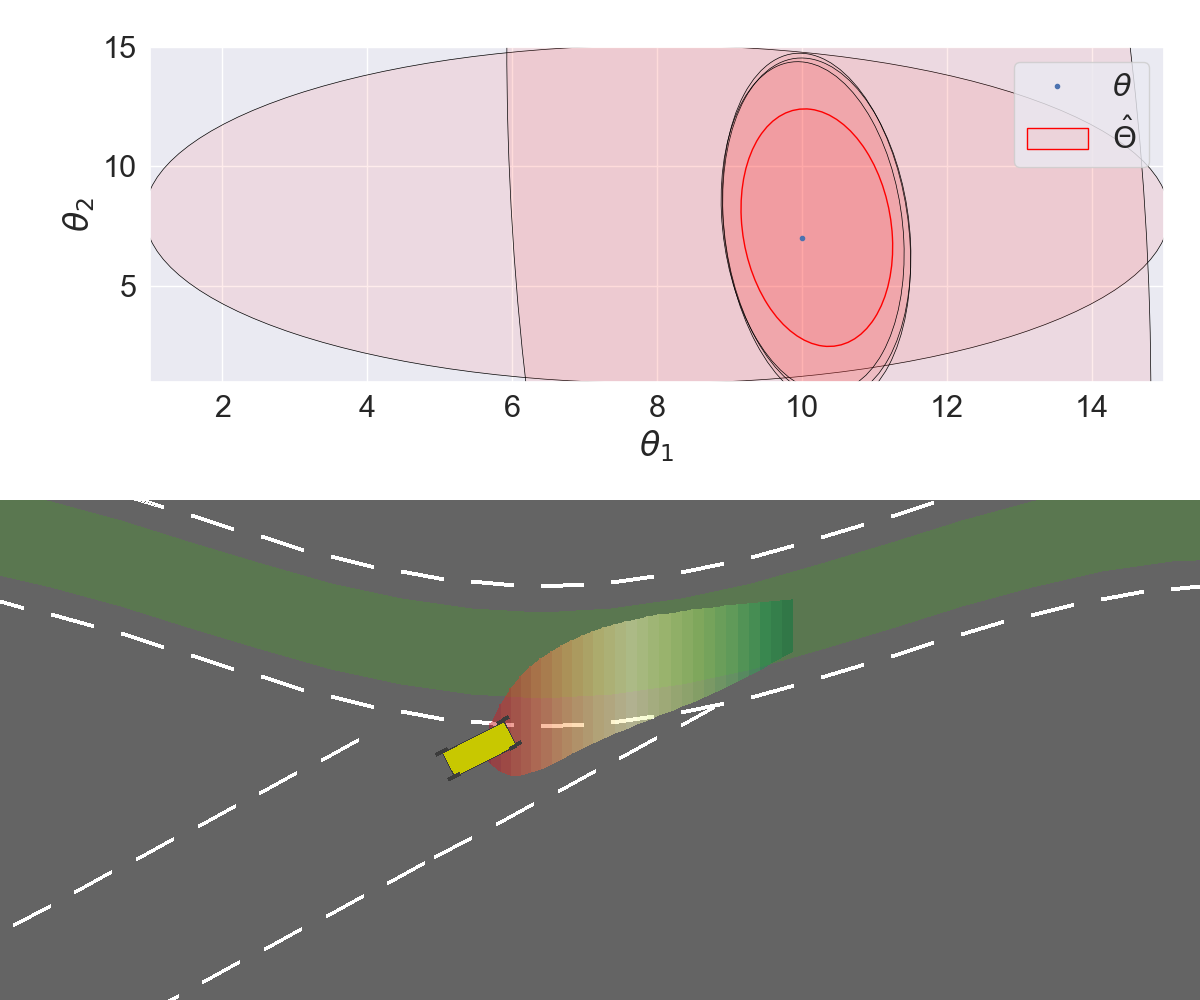
\includegraphics[width=0.9\linewidth]{img/lane-keeping.png}
	\caption{\textbf{Top}: the model estimation showing the confidence region $\confidenceset$ from \eqref{eq:predictor} at different times $t_N$. \textbf{Bottom}: a lane keeping application, where a car must follow a lane-center curve under unknown friction and perturbations. $X_f$ is shown in green, and $\xi(t)$ as an area with a color gradient.}
	\label{fig:lane-keeping}
\end{figure}

We tackle the problem of the robust adaptive lateral control of an autonomous vehicle for a lane-keeping application, implemented in \highwayenv. In contrast with \Cref{chapter:3} where we adopted a kinematic standpoint and simply assumed that the vehicle acceleration could be controlled directly, we dive deeper into a dynamical description subjected to \emph{unknown} tire friction forces. We still represent the state of a rigid vehicle by its position $(p_x, p_y)$, its yaw angle $\psi$, its velocity $(v_x, v_y)$ in the body frame and yaw rate $r$, and additionally denote its mass as $m$, its moment of inertia as $I_z$, and its front and rear axle positions as $a,b$. We consider the Dynamical Bicycle Model described in \citep[, Chapter 3.2]{awan2014compensation}: the vehicle is moving at constant longitudinal speed $u$, and the lateral force $F_y$ of a tire with slip angle $\alpha$ is assumed to be linear with an unknown friction coefficient $C_\alpha$: $F_y = C_\alpha \alpha$. The slip angle of the front and rear tires are respectively denoted as $\alpha_f, \alpha_r$, along with the corresponding friction coefficients.
Under a small angle approximation for $\psi, \alpha_f, \alpha_r$, Newton's second law of motion yields the linear dynamics \eqref{eq:dynamics} with
% \begin{align*}
% \dot{v_y} &= \frac{-2(C_{\alpha_f} + C_{\alpha_r})}{m v_x} v_y + \frac{2(C_{\alpha_r}b - C_{\alpha_f}a)}{m v_x} r - v_x r + \frac{2}{m}u, \\
% \dot{r} &= \frac{2(C_{\alpha_r}b - C_{\alpha_f}a)}{I_z v_x} v_y + \frac{-2(C_{\alpha_f}a^2 + C_{\alpha_r}b^2)}{I_z v_x} r + \frac{a}{I_z} u.
% \end{align*}
% We can rewrite them as

\[
x = \begin{bmatrix} {p_y} \\ {\psi} \\ {v_y} \\ {r} \end{bmatrix},\quad
\theta = \begin{bmatrix} C_{\alpha_f} \\ C_{\alpha_r}\end{bmatrix},\quad
A = \begin{bmatrix}
0 & v_x & 1 & 0 \\
0 & 0 & 0 & 1 \\
0 & 0 & 0 & - v_x \\
0 & 0 & 0 & 0
\end{bmatrix},\quad
B =
\begin{bmatrix}
0 \\
0 \\
\frac{2}{m} \\
\frac{a}{I_z}
\end{bmatrix},
\]

\[
\phi_1 = \frac{-2}{m v_x I_z}\begin{bmatrix}
0 & 0 & 0 & 0 \\
0 & 0 & 0 & 0 \\
0 & 0 & I_z & a I_z \\
0 & 0 & a m & a^2 m \\
\end{bmatrix},
\quad
\phi_2 = \frac{-2}{m v_x I_z}\begin{bmatrix}
0 & 0 & 0 & 0 \\
0 & 0 & 0 & 0 \\
0 & 0 & I_z & -b I_z \\
0 & 0 & - bm & b^2 m \\
\end{bmatrix}.
\]

\noindent Instead of simply stabilising the vehicle state $x$, we track the lateral position $y_r(t)$ of the lane centre. However, we do not have access to a full state reference $x_r(t) = [y_r(t), \psi_r(t), v_{y,r}(t), r_r(t)]^\transp$ consistent with the dynamics \eqref{eq:dynamics}. Thus, we define the state $\tilde{x} = x - [y_r(t), 0, 0, 0]^\transp$ and consider the remaining unknown terms $[0, \psi_r(t), v_{y,r}(t), r_r(t)]$ and $u_r(t)$ as perturbations $\omega(t)$, bounded since $x_r,\,u_r$ are assumed to belong to $\safestates = \pm[3, 2, 6, 6]^\transp$ and $\safecontrols=\pm[10]$.

The \Cref{fig:lane-keeping} depicts our approach. The confidence region $\confidenceset$ from \eqref{eq:confidence-ellipsoid} is shown in the top graph, and shrinks with time. To simplify verification of \Cref{assumpt:metzler} for this example, an auxiliary preliminary feedback has been applied shifting the eigenvalues of the closed-loop system. The robust stability of this feedback is assessed with the \gls{LMI} of \Cref{thm:ISS_pr}, and we compute the corresponding basin of attraction $X_f$ from \eqref{eq:X_f}, represented in green in the bottom subfigure. Then, we use a sampling-based \gls{MPC} scheme \citep{HomemDeMello2014} to solve \eqref{eq:OCP} and bring $\xi(t)$ into $X_f$ in $T=\SI{3}{\second}$.  The associated interval prediction $\xi(t)$ from \eqref{eq:predictor} is represented with a colour gradient from $t=t_n$ (red) to $t=t_n+T$ (green). Once the vehicles enters $X_f$, we finally switch to the closed-loop feedback \eqref{eq:control_pr} following \eqref{eq:control} for the rest of the simulation\footnote{A video is available at \href{https://youtu.be/axurBzHRLGY}{https://youtu.be/axurBzHRLGY}}.

\FloatBarrier
\section{Minimax control with generic costs}
\label{sec:control}

As we discussed in \Cref{sec:robust-motivation}, the ability to stabilise a system in the neighbourhood of the origin is not sufficient to tackle many tasks for which there exist no clear notion of equilibrium, and where the system must continually and dynamically adapt to its surroundings. This especially includes tasks akin to obstacle avoidance, which constitutes a substantial part of motion planning.

Therefore, in this section and as a second application of the tools introduced in \Cref{sec:estimation,sec:prediction}, we tackle the arguably more expressive objective of minimax control \eqref{eq:minimax-obj} of an arbitrary bounded reward function $\reward:\Real^p\to[0, 1]$, recalled here:
\begin{equation}
\hlg{\sup_{bu\in{(\Real^q)}^\Natural}} \hlr{\inf_{\substack{\theta \in \confidenceset \\ \bom\in[\underline{\bom},\overline{\bom}]^\Natural}}} \left[\sum_{n=N+1}^\infty \gamma^n R(x_n(\bu,\bom))\right]. \tag{\ref{eq:minimax-obj}}
\end{equation}

\paragraph{Evaluation} In order to evaluate this robust objective $V^r$, we approximate it thanks to the interval prediction $[\ux(t), \ox(t)]$ of \Cref{sec:prediction}.

\begin{definition}[Surrogate objective]
	\begin{leftbar}[defnbar]
	Let
	\begin{align}
	\label{eq:surrogate_objective} 
	\hat{V}^r(\bu) &\eqdef \sum_{n=N+1}^\infty \discount^n \pessimisticreward_n(\bu),\\ 
	\text{where}\quad\pessimisticreward_n(\bu) &\eqdef \min_{x\in[\ux_n(\bu), \ox_n(\bu)]}  \R(x), \label{eq:pessimistic-rewards}
	\end{align}
	and $\ux_n(\bu), \ox_n(\bu)$ follow the dynamics defined in \eqref{eq:interval-predictor}.
	\end{leftbar}
\end{definition}

This amounts to changing the reward function, except that the worst case is assessed over the whole past trajectory, which makes this pessimistic reward $\pessimisticreward_n$ \emph{not Markovian}.

\begin{proposition}[Lower bound]
	\label{prop:lower-bound}
	\begin{leftbar}[propositionbar]
	The surrogate objective  \eqref{eq:surrogate_objective} is a lower bound of the true objective  \eqref{eq:minimax-obj}: 
	\begin{equation*}
	\hat{V}^r(\bu) \leq V^r(\bu)
	\end{equation*}
	\end{leftbar}
\end{proposition}
A direct consequence is that since all our approximations are conservative, if we manage to find a control sequence such that no \emph{\enquote{bad event}} (\eg a collision) happens according to the surrogate objective $\hat{V}^r$, then we are guaranteed that they will not happen either when the controls are executed on the true system.
\begin{proof}
	We provide a proof in \Cref{sec:proof-lower-bound}.
\end{proof}

\paragraph{Planning}

\begin{algorithm}[t]
	\DontPrintSemicolon
	\caption{Integrated framework for confident estimation, interval prediction and minimax control}
	\label{alg:full}
	
	\KwData{confidence level $\confidence$, structure $(A,\phi)$, reward $R$, $\cD_{[0]}\gets\emptyset,\, \ba_1\gets\emptyset$}
	\For{$N = 0,1,2,\dots$}{
		$\confidenceset \gets$\textsc{Model Estimation}$(\cD_{[N]})$. \eqref{eq:confidence-ellipsoid}\;
		\For{each planning step $k\in\{N,\dots,N+K\}=N+[K]$}{
			$[\ux_{k+1}, \ox_{k+1}]\gets$ \textsc{Interval Prediction}($\confidenceset, \ba_kb$) for each action $b\in \cA$. \eqref{eq:interval-predictor}\;
			$\ba_{k+1}$ $\gets$\textsc{Pessimistic Planning}$(\underline{R_{k+1}}([\ux_{k+1}, \ox_{k+1}]))$.  \eqref{eq:opd}\;
		}
		Execute the recommended control $u_{N+1}$, and add the transition $(x_{N+1}, y_{N+1}, u_{N+1})$ to $\cD_{[N+1]}$.\;
	}
	
\end{algorithm}

To optimise $\hat{V}^r$ \eqref{eq:surrogate_objective}, we cannot use Dynamic Programming algorithms since the state space is continuous and the pessimistic rewards are non-Markovian. Instead, as we did in \Cref{chapter:6}, we turn to tree-based planning algorithms, which optimise a sequence of actions based on the corresponding sequence of rewards, without requiring Markovity nor state enumeration.

Though there exist works addressing continuous action spaces \citep{Busoniu2018,Weinstein2012}, we resort to a first approximation and discretise the continuous decision space $\Real^q$ by adopting a hierarchical control architecture: at each time, the agent can select a high-level \emph{action} $a$ from a finite space $\cA$. Each action $a\in\cA$ corresponds to the selection of a low-level controller $\pi_a$, that we take affine: $u(t) = \pi_a(x(t)) \eqdef -K_a x(t) + u_a.$ For instance, a tracking a subgoal $x_g$ can be achieved with $\pi_g = K(x_g - x)$. This discretisation induces a suboptimality, but it can be mitigated by diversifying the controller basis.
The robust objective \eqref{eq:minimax-obj} becomes
\[\sup_{\ba\in{\cA}^\Natural} V^r(\ba),\]
where $x_n(\ba, \bom)$ stems from \eqref{eq:dynamics} with $u_n = \pi_{a_n}(x_n)$.

This enables us to consider the \OPD algorithm \citep{Hren2008} tailored for the case when the relationship between actions and rewards is deterministic. Indeed, the stochasticity of perturbations and measurements is encased in $\hat{V}^r$: given the observations up to time $N$, both the predictor dynamics \eqref{eq:interval-predictor} and the pessimistic rewards \eqref{eq:pessimistic-rewards} are deterministic.

At each planning iteration $k\in[K]$, \OPD progressively builds a tree $\cT_{k+1}$ by forming upper-bounds $U_a(k)$ over the value of sequences of actions $a$, and expanding\footnote{The expansion of a leaf node $a$ refers to the simulation of its children transitions $a\cA = \{ab, b\in \cA\}$} the leaf $a_k$ with highest upper-bound:
\begin{equation}
\label{eq:opd}
a_k = \argmax_{a\in\cL_k} U_a(k), \quad U_a(k) = \sum_{n=0}^{h(a)-1} \pessimisticreward_n(a) + \frac{\discount^{h(a)}}{1-\discount}
\end{equation}
where $\cL_k$ is the set of leaves of $\cT_k$, $h(a)$ is the length of the sequence $a$, and $\pessimisticreward_n(a)$ the pessimistic reward \eqref{eq:pessimistic-rewards} obtained at time $n$ by following the controls $u_n = \pi_{a_n}(x_n)$.

\Cref{alg:full} shows the full integration of the three procedures of estimation, prediction and control. 

\begin{theorem}[Planning performance of \citealp{Hren2008}]
	\label{theorem:opd-regret}
	\begin{leftbar}[theorembar]
	The simple regret of the \OPD algorithm \eqref{eq:opd} applied to the surrogate objective \eqref{eq:surrogate_objective} after $K$ planning iterations is
	\begin{align*}
	\text{if } \kappa>1,\quad& 
	\hat{V}^r(a^{\star}) - \hat{V}^r({a_K}) = \cO\left(K^{-\frac{\log 1/\discount}{\log \kappa}}\right);\\
	\text{if }\kappa=1,\quad&
	\hat{V}^r(a^{\star}) - \hat{V}^r({a_K}) = \cO\left(\discount^{{(1-\discount)^{\log_\discount (\kappa/|\cA|)}}K/{c}}\right)
	\end{align*}
	where $\kappa$ is a problem-dependent measure of the proportion of near-optimal paths:
	\[
	\kappa = \limsup_{h\rightarrow\infty} \left|\left\{a\in A^h: \hat{V}^r(a)\geq \hat{V}^r(a^{\star}) - \frac{\discount^{h+1}}{1-\discount}\right\}\right|^{1/h}.
	\]
	\end{leftbar}
\end{theorem}
\begin{proof}
	We provide a proof in \Cref{sec:proof-regret-opd}.
\end{proof}

Hence, by using enough computational budget $K$ for planning we can get as close as we want to the optimal surrogate value $\hat{V}^r(a^{\star})$, at a polynomial rate. Unfortunately, there exists a gap between $\hat{V}^r$ and the true robust objective $V^r$, which stems from three approximations: (i) the true reachable set was approximated by an enclosing interval in \eqref{eq:inclusion-property}; (ii) the time-invariance of the dynamics uncertainty $\structureddynamics\in\confidenceset$ was handled by the interval predictor \eqref{eq:interval-predictor} as if it were a time-varying uncertainty $A(\theta(t))\in\confidenceset,\forall t$ ; and (iii) the lower-bound $\sum\min\leq \min\sum$ used to define the surrogate objective \eqref{eq:surrogate_objective} is not tight. However, this gap can be bounded with additional assumptions.

\begin{theorem}[Regret bound]
	\label{thm:minimax-regret-bound}
	\begin{leftbar}[theorembar]
	Under two conditions:
	\begin{enumerate}
		\item a Lipschitz regularity assumption for the reward $R$:
		\item a stability condition: there exist $P>0,Q_0\in\Real^{p\times p}$, $\rho>0$ such that
		$$\begin{bmatrix}
		A_0^\transp P + P A_0^\transp + Q_0 & P|D|  \\
		|D|^\transp P & -\rho I_r \\
		\end{bmatrix}< 0;$$
	\end{enumerate}
	we can bound the suboptimality of \Cref{alg:full} with planning budget $K$ as:
	\begin{equation*}
	\hat{V}^r(a_K) \leq {V}^r(a^\star) \leq V(a^\star) \leq \hat{V}^r(a_K) + \hlr{\underbrace{\Delta_\omega}_{\substack{\text{robustness to}\\ \text{perturbations}}}} + \hlb{\underbrace{\cO\left(\frac{\beta_N(\delta)^2}{\lambda_{\min}(\gls{gramian})}\right)}_{\text{estimation error}}} + \hlg{\underbrace{\cO\left(K^{-\frac{\log 1/\discountfactor}{\log \kappa}}\right)}_{\text{planning error}}}
	\end{equation*}
	with probability at least $1-\confidence$, where $\hlr{\Delta_\omega}$ is a constant which corresponds to an irreducible suboptimality suffered from being robust to instantaneous perturbations $\omega(t)$.
	\end{leftbar}
\end{theorem}
\begin{proof}
	We provide a proof in \Cref{sec:proof-minimax-regret-bound}.
\end{proof}

This bound contains an input-dependent estimation error term, which can be further bounded under an additional assumption that the features are sufficiently excited. 

\begin{corollary}[Persistent excitation]
	\label{cor:pe}
	\begin{leftbar}[corollarybar]
	Under an additional persistent excitation (PE) assumption
	\begin{align*}
	\exists \underline{\phi},\overline{\phi}>0: \forall n\geq n_0,\quad \underline{\phi}^2 \leq \lambda_{\min}(\Phi_{n}^\transp\Sigma_{p}^{-1}\Phi_{n}) \leq \overline{\phi}^2,
	\end{align*}
	the result of \Cref{thm:minimax-regret-bound} takes the more explicit form:
	\begin{equation*}
	\hat{V}^r(a_K) \leq {V}^r(a^\star) \leq V(a^\star) \leq \hat{V}^r(a_K) + \hlr{\underbrace{\Delta_\omega}_{\substack{\text{robustness to}\\ \text{perturbations}}}} + \hlb{\underbrace{\cO\left(\frac{\log\left(N^{d/2}/\confidence\right)}{N}\right)}_{\text{estimation error}}} + \hlg{\underbrace{\cO\left(K^{-\frac{\log 1/\discountfactor}{\log \kappa}}\right)}_{\text{planning error}}}
	\end{equation*}
	which ensures asymptotic near-optimality when $N\to\infty$ and $K\to\infty$.
	\end{leftbar}
\end{corollary}
\begin{proof}
	We provide a proof in \Cref{sec:proof-pe}.
\end{proof}

\section{Multi-model selection}
\label{sec:multi-model}

The procedure we developed in \Cref{sec:estimation,sec:prediction,sec:control} relies on strong modelling assumptions, such as the dynamics structure in \Cref{assumpt:structure}. But what if they are wrong?

\paragraph{Model adequacy}

One of the major benefits of using the family of linear models, compared to richer model classes, is that they provide strict conditions allowing to quantify the adequacy of the modelling assumptions to the observations.

Given $N-1$ observations, \Cref{sec:estimation} provides a polytopic confidence region \eqref{eq:polytope} that contains $\structureddynamics$ with probability at least $1-\confidence$. Since the dynamics are linear, we can propagate this confidence region to the next observation: $y_{N}$ must belong to the Minkowski sum of a polytope representing model uncertainty $\cP(A_{0} x_N + Bu_N, \Delta A_{1}x_N,\dots, \Delta A_{2^d}x_N)$ and a polytope $\cP(0_p, \underline{\eta}, \overline{\eta})$ bounding the perturbation and measurement noises. \citet{delos2015} provide a way to test this membership in polynomial time using linear programming. Whenever it is not verified, we can confidently reject the $(A,\phi)$-modelling \Cref{assumpt:structure}. This enables us to consider a rich set of potential features $\left((A^1, \phi^1), \dots, (A^M, \phi^M)\right)$ rather than relying on a single assumption, and only retain those that are consistent with the observations so far. Then, every remaining hypothesis must be considered during planning.

\paragraph{Robust selection}

We temporarily ignore the parametric uncertainty on $\theta$ to simply consider several candidate dynamics models, which all correspond to different modelling assumptions. We also restrict to deterministic dynamics, which is the case of \eqref{eq:interval-predictor}.

\begin{assumption}[Multi-model ambiguity]
	\label{assumpt:multi-model-ambiguity}
	\begin{leftbar}[assumptionbar]
	The true dynamics $f$ lies within a finite set of candidate models $f^1, \dots, f^M$.
	\begin{equation*}
	\exists m\in[M]: \dot{x}(t) = f^m(x(t), u(t)), \forall t\geq 0
	\end{equation*}
	\end{leftbar}
\end{assumption}
We want to adapt our planning algorithm in order to balance these concurrent hypotheses in a robust fashion, \ie maximise a robust objective with discrete ambiguity
\begin{equation}
\label{eq:robust-objective-discrete}
\hlg{\sup_{a\in\cA^\Natural}}\underbrace{\hlr{\min_{m\in[M]}} \sum_{n=N+1}^\infty \discount^n R_n^m}_{V^r(a)}
\end{equation}
where $R_n^m$ is the reward obtain by following the action sequence $a$ up to step $n$ under the dynamics $f^m$.
This objective could be optimised in the same way as in \Cref{sec:control}, but this would result in a coarse and lossy approximation. Instead, we exploit the finite uncertainty structure of \Cref{assumpt:multi-model-ambiguity} to asymptotically recover the true $V^r$ by modifying the \OPD algorithm in the following way:

\begin{definition}[Robust sequence upper bounds]
	\begin{leftbar}[defnbar]
	We replace the upper-bound \eqref{eq:opd} on sequence values in \OPD by
	\begin{equation}
	\label{eq:robust-b-values}
	U_a^r(k)  \eqdef \min_{m\in[M]} \sum_{n=0}^{h-1} \discount^n R_n^m  + \frac{\discount^h}{1-\discount}
	\end{equation}
	\end{leftbar}
\end{definition}
An illustration of the computation of the robust upper-bounds is presented in \Cref{fig:drop}. 
Note that it is not equivalent to solving each control problem independently and following the action with highest worst-case value:
\begin{remark}
	\label{sec:min-max-order}
	\begin{leftbar}[remarkbar]
	In the definition of $U_{a}^{r}(k)$ \eqref{eq:br} and $L_{a}^{r}(k)$ \eqref{eq:ur} it is essential that the minimum over the models is only taken at the end of trajectories, in the same way as for the robust objective \eqref{eq:robust-objective-discrete} in which the worst-case dynamics is only determined after the action sequence has been fully specified. Assume that $L_{a}^{r}(k)$ is instead naively defined as
	\[
	L_{a}^{r}(k)=\min_{m\in[1,M]}L_{a}^{m}(k),
	\]
	
	This would not recover the robust policy, as we show in \Cref{fig:min-max-order} with a simple counter-example.
\end{leftbar}
	\begin{figure}[htp]
	\centering
	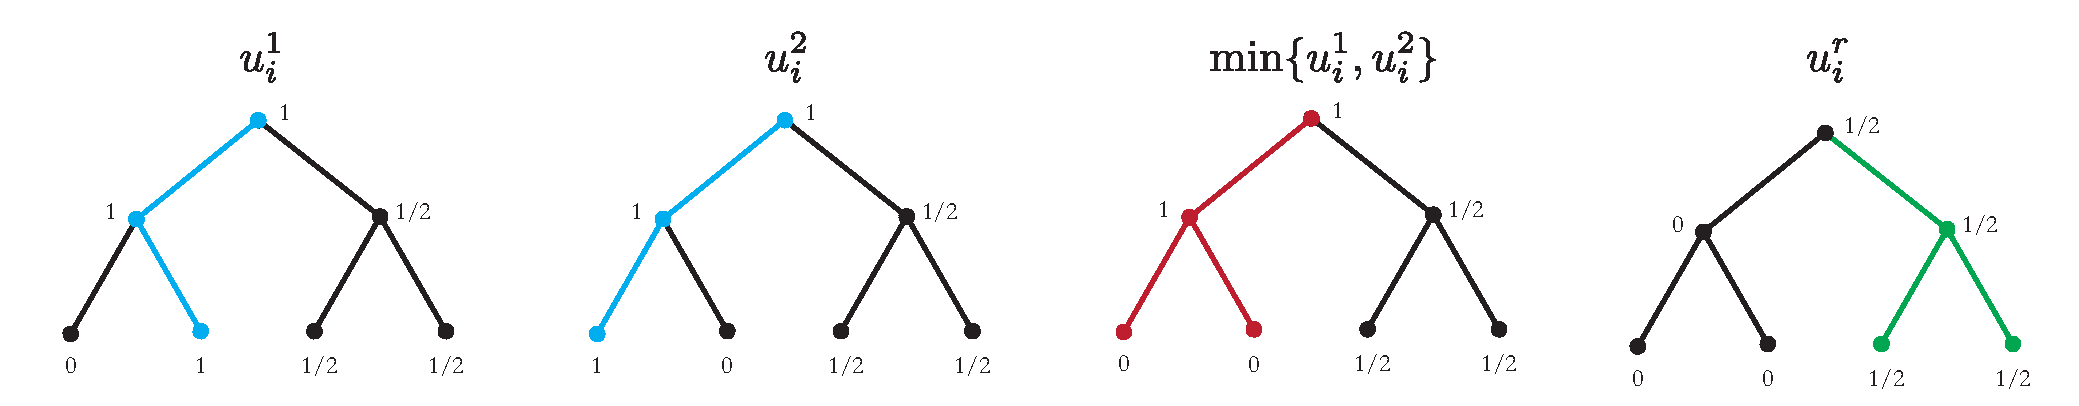
\includegraphics[width=\linewidth]{img/min-max-order}
	\caption{From left to right: two simple models and corresponding u-values with optimal sequences in blue; the naive version of the robust values returns sub-optimal paths in red; our robust U-value properly recovers the robust policy in green.}
	\label{fig:min-max-order}
	\end{figure}
\end{remark}

We analyse the sample complexity of the corresponding robust planning algorithm.

\begin{figure}
	\centering
	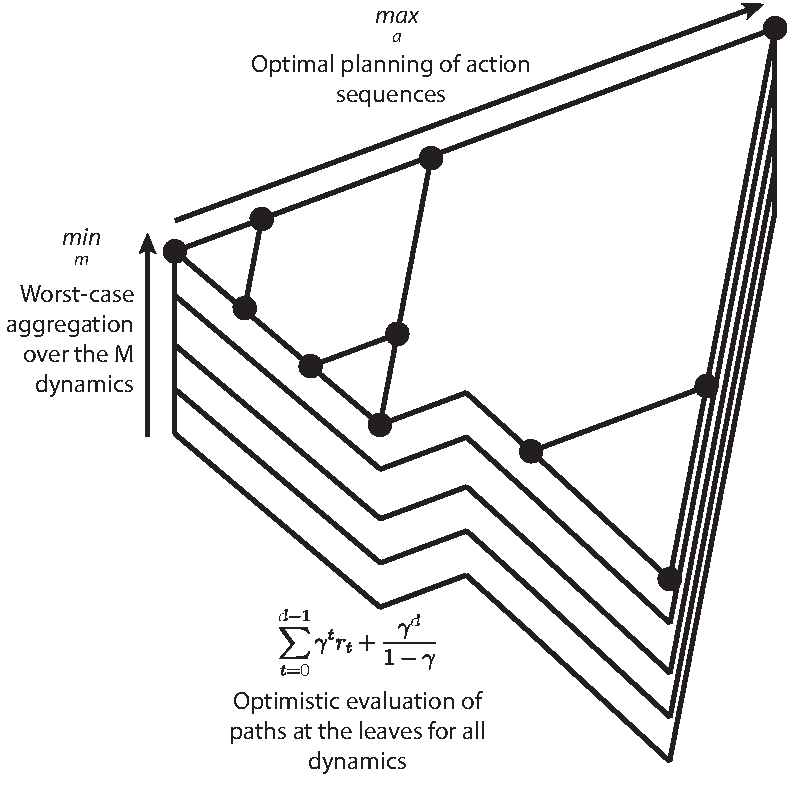
\includegraphics[width=0.45\linewidth]{img/robust-control-tree}
	\caption{The computation of robust U-values in \eqref{eq:robust-b-values}. The simulation of trajectories for every dynamics model $f^m$ is represented as stacked versions of the expanded tree $\mathcal{T}_k$.}
	\label{fig:drop}
\end{figure}

\begin{theorem}[Robust planning performance]
	\label{theorem:drop-regret}
	\begin{leftbar}[theorembar]
	The robust version of \OPD \eqref{eq:robust-b-values} enjoys the same regret bound as \OPD in \Cref{theorem:opd-regret}, with respect to the multi-model objective \eqref{eq:robust-objective-discrete}.
	\end{leftbar}
\end{theorem}
\begin{proof}
	We provide a proof in \Cref{sec:proof-drop-regret}.
\end{proof}

The regret depends on the number $K$ of node expansions, but each expansion now requires $M$ times more simulations than in the single-model setting. The solution of the robust objective \eqref{eq:robust-objective-discrete} with discrete ambiguity $f\in\{f^m\}_{m\in[M]}$ can be recovered exactly, asymptotically when the planning budget $K$ goes to infinity. This contrasts the results obtained in \Cref{sec:control} for the robust objective \eqref{eq:minimax-obj} with continuous ambiguity $\params\in\confidenceset$, for which \OPD only recovers the surrogate approximation $\hat{V}^r$, as discussed in \Cref{thm:minimax-regret-bound}. Finally, the two approaches of \Cref{sec:control,sec:multi-model} can be merged by using the pessimistic reward \eqref{eq:pessimistic-rewards} in \eqref{eq:robust-b-values}.

\section{Experiments}
\label{sec:interval-experiments}

\paragraph{Obstacle avoidance with unknown friction}
We first consider a simple illustrative example, shown in \Cref{fig:prediction}: the control of a 2D system with position $(p_x,p_y)$ and velocity $(v_x, v_y)$ moving by means of a force $(u_x, u_y)$ in an environment with unknown anisotropic friction.

\begin{equation*}
\begin{bmatrix}
\dot{p_x}\\
\dot{p_y}\\
\dot{v_x}\\
\dot{v_y}\\
\end{bmatrix} = 
\begin{bmatrix}
0 & 0 & 1 & 0 \\
0 & 0 & 0 & 1 \\
0 & 0 & -\theta_x & 0 \\
0 & 0 & 0 & -\theta_y
\end{bmatrix}
\begin{bmatrix}
{p_x}\\
{p_y}\\
{v_x}\\
{v_y}\\
\end{bmatrix}
+
\begin{bmatrix}
0\\
0\\
{u_x}\\
{u_y}\\
\end{bmatrix}
\end{equation*}

Note that the \Cref{assumpt:metzler} for $A_0$ is always verified. The reward is non-smooth and encodes the task of navigating to reach a goal state $x_g$ while avoiding collisions with obstacles: $\R(x) = \delta(x)/(1 + \|x - x_g\|_2)$  where $\delta(x)$ is $0$ whenever $x$ collides with an obstacle, $1$ otherwise. The actions $\cA$ are constant controls in the up, down, left and right directions. The environment is illustrated in \Cref{fig:obstacle-env}.

\begin{figure}[ht]
	\centering
	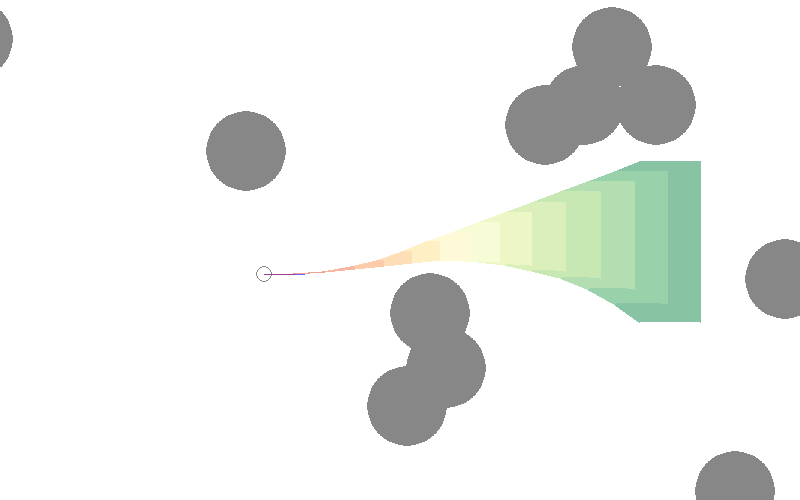
\includegraphics[width=0.7\linewidth]{img/obstacle_small}
	\caption{\Cref{alg:full} running on the obstacle avoidance environment: we show the predicted state interval at each prediction time step (from \hlr{red} to \hlg{green}).}
	\label{fig:obstacle-env}
\end{figure}

We run \Cref{alg:full} for 100 simulations, and compare in \Cref{tab:obstacle} its performances to that of the nominal agent, \ie the non-robust adaptive control approach that plans with the estimated dynamics $\theta_{[N],\lambda}$. We observe that though the robust agent performs worse than the nominal agent on average, it manages to ensure safety and attains a better worst-case performance, as intended. We also study the evolution of the simple regret $V(x_n) - J_n(x_n)$ with respect to the number of samples $N$, where $J_n(x_n) = \sum_{i > n} \discount^i R_i$ is the empirical return at state $x_n$ in a trajectory $x_0, R_0, x_1, R_1, \dots$, while $V(x_n)$ is the optimal value that the agent would get by acting optimally from $x_n$ with knowledge of the dynamics. The mean regret is shown in \Cref{fig:regret}, along with its \SI{95}{\percent} confidence interval. We see that \Cref{alg:full} has a regret $\hat{V}^r - V$ decreasing at least polynomially with $N$, as expected from \Cref{thm:minimax-regret-bound}. This shows that the agent gets more aggressive when it is more confident, as desired, while ensuring safety at all time. In contrast, the nominal agent has an even smaller regret but collided with obstacles in \SI{4}{\percent} of simulations\footnote{A video is available at \href{https://youtu.be/OY0yN3CuHFs}{https://youtu.be/OY0yN3CuHFs}. It compares trajectories of the oracle planner, nominal planner, and \Cref{alg:full}. The oracle planner has access to the true dynamics and follows aggressive trajectories that nearly saturate the collision constraints. The nominal planner trusts the estimated dynamics, which leads to collisions. In contrast, the \Cref{alg:full} produces more conservative trajectories. We show the confidence ellipsoid over $\theta = (\theta_x,\theta_y)$ in the right panel.}.

\begin{figure}[tp]
	\centering
	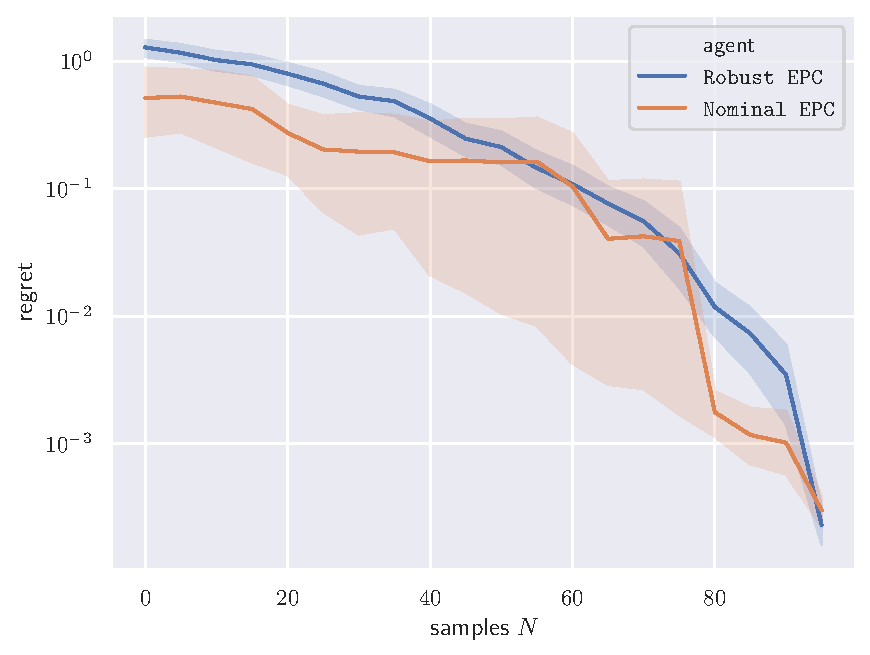
\includegraphics[width=0.8\linewidth]{img/regret.pdf}
	\caption{The mean regret along with its $95\%$ confidence interval with respect to $N$, for the robust and nominal agents.}
	\label{fig:regret}
\end{figure}

\begin{table}[tbp]
	\caption{Performances on the obstacle avoidance task}
	\label{tab:obstacle}
	\centering
	\begin{tabular}{lccc}
		\toprule
		Agent &
		failures &
		min return &
		mean return $\pm$ std  \\
		\midrule
		Oracle & 0\% & {11.6} & {$14.2 \pm 1.3$} \\
		\midrule
		{Nominal} & {4\%} & {2.8} & \textbf{$\mathbf{13.8} \pm 2.0$} \\
		\Cref{alg:full} & \textbf{0\%} & \textbf{10.4} & {$13.0 \pm 1.5$} \\
		\bottomrule
	\end{tabular}
\end{table}

\paragraph{Behavioural planning for an autonomous vehicle}
We consider the \href{https://github.com/eleurent/highway-env}{highway-env} environment \citep{highway-env} for simulated driving decision problems. An autonomous vehicle with state $x_0\in\Real^4$ is approaching an intersection among ${N_v}$ other vehicles with states $x_i\in\Real^4$, resulting in a joint traffic state $x = [x_0, \dots,x_{N_v}]^\top\in\Real^{4{N_v}+4}$. These vehicles follow parametrized behaviours $\dot{\chi}_i=f_i(x,\theta_i)$ with unknown parameters $\theta_i\in\Real^5$. We appreciate a first advantage of the structure imposed in \Cref{assumpt:structure}: the uncertainty space of $\theta$ is $\Real^{5{N_v}}$. In comparison, the traditional LQ setting where the whole state matrix $A$ is estimated would have resulted in a much larger parameter space $\theta\in\Real^{16{N_v}^2}$.
%This allows to scale to larger systems: in our experiments, we used a state space of dimension $44$ ($V=10$) where \eg \citep{Dean2018,abeille18a} reported numerical experiments with states of dimensions 3 and 4, respectively.
The system dynamics $f$, which describes the couplings and interactions between vehicles, can only be expressed in the form of \Cref{assumpt:structure} given the knowledge of the desired route for each vehicle, with features $\phi$ expressing deviations to the centerline of the followed lane. Since these intentions are unknown to the agent, we adopt the multi-model perspective of \Cref{sec:multi-model} and consider one model per possible route for every observed vehicle before an intersection. We compare \Cref{alg:full} to a nominal agent planning with the estimated parameter $\theta_{[N],\lambda}$, with two different modelling assumptions: we assume that Nominal 1 has access to the true followed route for each vehicle, while Nominal 2 does not and picks a model with minimal prediction error. Their performances are compared in \Cref{tab:driving}. Again, the robust approach is less efficient on average than planning with a nominal model, but it does better in terms of worst-case performance and manages to avoid collisions, contrary to the nominal baselines that suffer from model bias \footnote{A video is available at \href{https://youtu.be/0z65DCE1XWM}{https://youtu.be/0z65DCE1XWM}, comparing oracle and robust planners. We show the multi-model rejection and robust selection procedure through the display of several trajectory hulls for all possible destinations of the observed vehicles.}.

\begin{figure}[t]
	\centering
	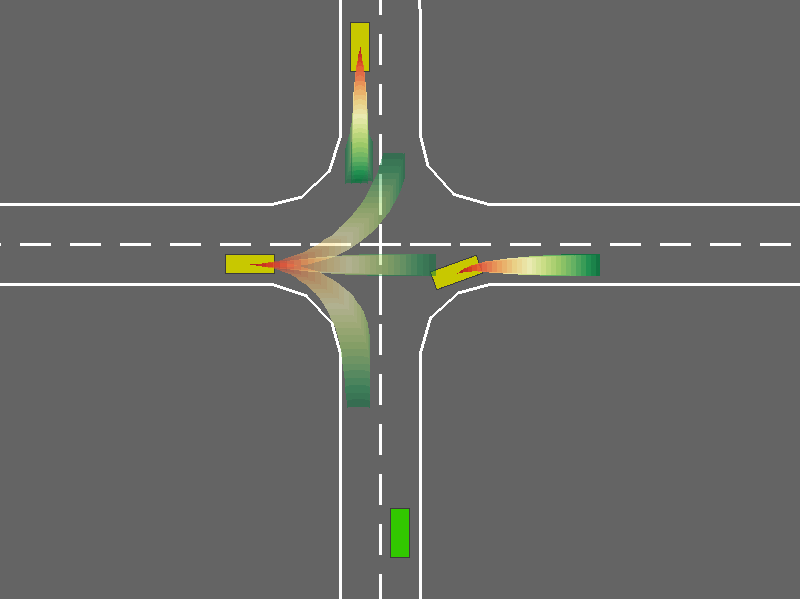
\includegraphics[width=0.7\linewidth]{img/highway-small}
	\caption{The intersection crossing task. We show the trajectory intervals corresponding to behavioural uncertainty for each observed vehicle, and the multi-model assumption over the followed route.}
\end{figure}

\begin{table}[t]
	\caption{Performances on the driving task}
	\label{tab:driving}
	\centering
	\begin{tabular}{lccc}
		\toprule
		Agent &
		failures &
		min return &
		mean return $\pm$ std  \\
		\midrule
		Oracle & 0\% & {6.9} & $7.4 \pm 0.5$ \\
		\midrule
		{Nominal 1} & 4\% & {5.2} & $\mathbf{7.3} \pm 1.5$ \\
		{Nominal 2} & 33\% & {3.5} & $6.4 \pm 0.26$ \\
		\Cref{alg:full} & \textbf{0\%} & \textbf{6.8} & $7.1 \pm 0.29$ \\
		\bottomrule
	\end{tabular}
\end{table}

\section*{Chapter conclusion}

We propose a framework for the robust estimation, prediction and control of a partially known linear system. After deriving a confidence region for the state matrix through non-asymptotic linear regression, we design an interval predictor guaranteed to contain the induced trajectory, and whose stability is guaranteed upon satisfaction of an \gls{LMI}. We leverage these tools in two applications. First, the robust stabilisation of the system at the origin under state and control constraints, that we achieve with a dual \gls{MPC} and feedback that both exploit the predicted intervals. Second, the minimax control of a generic (non-quadratic) cost function, for which we provide a tree-based planning algorithm whose predicted performance is guaranteed and whose regret is bounded. The applicability of the method is further improved by a multi-model extension and demonstrated on several simulated driving applications, namely: socially-aware trajectory prediction for an observed vehicle, steering control under unknown tire friction, and safe intersection crossing among drivers with uncertain destination and driving styles.

%\begin{subappendices}
%%!TEX root = ../../PhD_thesis__Edouard_Leurent.tex
\graphicspath{{2-Chapters/7-Chapter/}}
	
\chapter{Complements on \Cref{chapter:7}}
	\section{Proofs}
	
	\subsection{Proof of \Cref{prop:regularized_solution}}
	\label{sec:proof-regularized_solution}
	
	\begin{proof}
		We differentiate $J(\theta) = \sum_{n=1}^N \|y_n -\Phi_n\theta\|_{\Sigma_p^{-1}}^2 + \lambda\|\theta\|_{}^2$ as in  \eqref{eq:regression_min} with respect to $\theta$:
		
		\begin{align*}
		\nabla_{\theta} J(\theta) &= \sum_{n=1}^N\nabla_{\theta} (y_n - \Phi_n\theta)^\transp\Sigma_p^{-1}(y_n - \Phi_n\theta) + \nabla_{\theta} \lambda\|\theta\|_{}^2\\
		&= -2\sum_{n=1}^N y_n^\transp\Sigma_p^{-1}\Phi_n + 2\sum_{n=1}^N\theta^\transp(\Phi_n^\transp\Sigma^{-1}\Phi_n) +  2 \lambda \theta^\transp
		\end{align*}
		
		Hence,
		\begin{align*}
		\nabla_{\theta} J(\theta) = 0 \iff \left(\sum_{n=1}^N\Phi_n^\transp\Sigma_p^{-1}\Phi_n + I_d\right)\theta = \sum_{n=1}^N y_n^\transp\Sigma_p^{-1}\Phi_n
		\end{align*}
	\end{proof}
	
	\subsection{Proof of \Cref{thm:confidence_ellipsoid}}
	\label{sec:proof-confidence_ellipsoid}
	
	We start by showing a preliminary proposition:
	\newpage
	
	\begin{proposition}[Matrix version of Theorem 1 of \citealp{Abbasi2011}]
		\label{prop:concentration}
		\begin{leftbar}[propositionbar]
		Let $\{F_n\}_{n=0}$ be a filtration.
		Let $\{\eta_n\}_{n=1}^\infty$ be a $\Real^p$-valued stochastic process such that $\eta_n$ is $F_n$-measurable and $\expectedvalue\left[\eta_n\condbar F_{n-1}\right]$ is $\Sigma_p$-sub-Gaussian.
		
		Let $\{\Phi_n\}_{n=1}^\infty$ be an $\Real^{p\times d}$-valued stochastic process such that $\Phi_n$ is $F_n$-measurable. Assume that $G$ is a $d\times d$ positive definite matrix.
		For any $n\geq 0$, define
		\begin{equation*}
		\overline{G}_n = G + \sum_{s=1}^n \Phi_s^\transp \Sigma_p^{-1} \Phi_s \in \Real^{d\times d} \quad S_n = \sum_{s=1}^n \Phi_s^\transp\Sigma_p^{-1}\eta_s \in \Real^{d}.
		\end{equation*}
		Then, for any $\confidence>0$, with probability at least $1-\confidence$, for all $n\geq0$,
		\begin{align*}
		\| S_n \|_{\overline{G}_n^{-1}} \leq \sqrt{2\log \left(\frac{\det\left(\overline{G}_n\right)^{1/2}}{\confidence\det(G)^{1/2}}\right)}.
		\end{align*}
		\end{leftbar}
	\end{proposition}
	\begin{proof}
		Let 
		\begin{equation*}
		G_t = \sum_{s=1}^t \Phi_s^\transp \Sigma_p^{-1} \Phi_s \in \Real^{d\times d}
		\end{equation*}
		And for any $z\in\Real^d$,
		\begin{equation*}
		M_t^z = \exp{\left(\inp{z}{S_t} - \frac{1}{2}\|z\|_{G_t}\right)}
		\end{equation*}
		\begin{equation*}
		D_t^z = \exp{\left(\inp{\Phi_t z}{\eta_t}_{\Sigma_p^{-1}} - \frac{1}{2}\|\Phi_t z\|_{\Sigma_p^{-1}}\right)}
		\end{equation*}
		Then,
		\begin{align*}
		M_t^z &= \exp{\left(\sum_{s=1}^t z^\transp \Phi_s^\transp \Sigma_p^{-1} \eta_s - \frac{1}{2} (\Phi_s z)^\transp\Sigma_p^{-1}(\Phi_s z) \right)} \\
		&= \prod_{s=1}^{t} D_s^z
		\end{align*}
		and using the sub-Gaussianity of $\eta_t$
		\begin{align*}
		\expectedvalue\left[D_t^z \condbar F_{t-1}\right] = {}& \exp{\left(- \frac{1}{2}\|\Phi_t z\|_{\Sigma_p^{-1}}\right)}\\ &\expectedvalue\left[\exp{\left(\inp{\Phi_t z}{\eta_t}_{\Sigma_p^{-1}}\right)} \condbar F_{t-1}\right]  \\
		\leq {} & \exp{\left(- \frac{1}{2}\|\Phi_t z\|_{\Sigma_p^{-1}}\right)}\\
		&\exp{\left((z^\transp \Phi_t^\transp \Sigma_p^{-1})\Sigma_p(\Sigma_p^{-1} \Phi_t z)\right)}\\
		&= 1
		\end{align*}
		\begin{align*}
		\expectedvalue\left[M_t^z \condbar F_{t-1}\right] = \left(\prod_{s=1}^{t-1} D_s^z\right) \expectedvalue\left[D_t^z \condbar F_{t-1}\right] \leq M_{t-1}^z
		\end{align*}
		Showing that $(M_t^z)_{t=1}^\infty$ is indeed a supermartingale and in fact $\expectedvalue[M_t^z]\leq 1$.
		It then follows by Doob's upcrossing lemma for supermartingale that $M_\infty^z = \lim_{t\to\infty} M_t^z$ is almost surely well-defined, and so is $M_\tau^z$ for any random stopping time $\tau$.
		
		Next, we consider the stopped martingale $M_{\min(\tau,t)}^z$. Since 
		$(M_t^z)_{t=1}^\infty$ is a non-negative supermartingale and $\tau$ is a random stopping time, we deduce by Doob's decomposition that
		\begin{align*}
		\expectedvalue[M_{\min(\tau,t)}^z] &= \expectedvalue[M_0^z] + \expectedvalue[\sum_{s=0}^{t-1} (M_{s+1}^z-M_s^z) \mathbb{I}\{\tau>s\}]\\
		&\leq 1 + \expectedvalue[\sum_{s=0}^{t-1} \expectedvalue[M_{s+1}^z-M_s^z|F_{s}] \mathbb{I}\{\tau>s\}]\\
		&\leq 1
		\end{align*}
		Finally, an application of Fatou's lemma show that 
		$$\expectedvalue[M_\tau^z] = \expectedvalue[\liminf_{t\to\infty} M_{\min(\tau,t)}^z] \leq \liminf_{t\to\infty} \expectedvalue[M_{\min(\tau,t)}^z] \leq 1.$$
		
		This results allows to apply a result from \citep{pena2008self}.
		\begin{lemma}[Theorem 14.7 of \citealp{pena2008self}]
			\begin{leftbar}[lemmabar]
			If $Z$ is a random vector and $B$ is a symmetric positive definite matrix such that
			\[\forall \discount\in\Real^d, \log \expectedvalue \exp \left(\discount^\transp Z -\frac{1}{2} \discount^\transp B \discount \right)\leq 0,\]
			then for any positive definite non-random matrix C, it holds
			\[\expectedvalue\left[ \sqrt{\frac{\det(C)}{\det(B+C)} } \exp\left( \frac{1}{2}\|Z\|^2_{(B+C)^{-1}}\right)\right]\leq 1. \] 
			In particular, by Markov inequality, for all $\confidence\in(0,1)$, 
			\[\probability{\|Z\|_{(B+C)^{-1}} \geq \sqrt{2\log \left(\frac{\det \left((B+C)^{1/2}\right)}{\confidence\det(C)^{1/2}}\right)}}\leq \confidence.\]
			\end{leftbar}
		\end{lemma}
		
		Here, by using $Z = \sum_{s=1}^t\Phi_s\Sigma_p^{-1}\eta_s$, $B=G_t$, $C=G$,
		
		\[
		\probability{\| S_t \|_{(G_t+G)^{-1}} \geq \sqrt{2\log \left(\frac{\det(G_t+G)^{1/2}}{\confidence\det(G)^{1/2}}\right)}} \leq \confidence
		\]
		
	\end{proof}
	
	Having shown this preliminary result, we move on to the proof of \Cref{thm:confidence_ellipsoid}.
	
	\begin{proof}
		For all $x\in\Real^d$, \eqref{eq:vector_rls} gives
		\begin{align*}
		x^\transp\theta_{N,\lambda}  -x^\transp\theta &= x^\transp G_{N, \lambda}^{-1}\sum_{n=1}^N \Phi_n^\transp \Sigma_p^{-1}\eta_n
		- \lambda x^\transp G_{N, \lambda}^{-1}\theta\\
		&= \inp{x}{\sum_{n=1}^N \Phi_n^\transp \Sigma_p^{-1}\eta_n}_{G_{N, \lambda}^{-1}} - \lambda\inp{x}{\theta}_{G_{N, \lambda}^{-1}}
		\end{align*}
		
		Using the Cauchy-Schwartz inequality, we get
		\begin{align*}
		|x^\transp\theta_{N,\lambda}  -x^\transp\theta| \leq \|x\|_{G_{N, \lambda}^{-1}}\left(\left\|\sum_{n=1}^N \Phi_n^\transp \Sigma_p^{-1}\eta_n\right\|_{G_{N, \lambda}^{-1}} + \lambda\|\theta\|_{G_{N, \lambda}^{-1}}\right)
		\end{align*}
		
		In particular, for $x = G_{N,\lambda}(\theta_{N,\lambda} - \theta)$, we get after simplifying with $\| \theta_{N,\lambda}  - \theta\|_{G_{N,\lambda}}$,
		\begin{align*}
		\| \theta_{N,\lambda}  - \theta\|_{G_{N,\lambda}} &\leq \left\|\sum_{n=1}^N \Phi_n^\transp \Sigma_p^{-1}\eta_n\right\|_{G_{N, \lambda}^{-1}} + \lambda\|\theta\|_{G_{N, \lambda}^{-1}}
		\end{align*}
		
		By applying \Cref{prop:concentration} with $G=\lambda I_d$, we obtain that with probability at least $1-\confidence$,
		\begin{align*}
		\| \theta_{N,\lambda}  - \theta\|_{G_{N,\lambda}} &\leq \sqrt{2\log \left(\frac{\det(G_{N,\lambda})^{1/2}}{\confidence\det(\lambda I_d)^{1/2}}\right)}
		+ \lambda\|\theta\|_{G_{N, \lambda}^{-1}}
		\end{align*}
		And since $\|\theta\|_{G_{N, \lambda}^{-1}}^2 \leq 1/\lambda_{\min}(G_{N,\lambda})\|\theta\|_2^2 \leq 1/\lambda \|\theta\|_2^2$ and $\|\theta\|_2^2 \leq d\|\theta\|_\infty^2\leq d S^2$,
		\begin{align*}
		\| \theta_{N,\lambda}  - \theta\|_{G_{N,\lambda}} &\leq \sqrt{2\log \left(\frac{\det(G_{N,\lambda})^{1/2}}{\confidence\det(\lambda I_d)^{1/2}}\right)}
		+ (\lambda d)^{1/2}S
		\end{align*}
	\end{proof}
	
	
	\subsection{Proof of \Cref{prop:lower-bound}}
	\label{sec:proof-lower-bound}
	\begin{proof}
		The predictor designed in \Cref{sec:prediction} verifies the inclusion property \eqref{eq:inclusion-property}. Thus, for sequence of controls $\bu$, any dynamics $\structureddynamics\in C_{[N],\confidence}$, and perturbations $\underline{\bom} \leq \bom \leq \overline{\bom}$, the corresponding state at time $t_n$ is bounded by $\underline{x}_n \leq x_n \leq \overline{x}_n$, which implies that $R(x_n) \geq \min_{x\in[\underline{x}_n(\bu), \overline{x}_n(\bu)]}  R(x) = \pessimisticreward_n(\bu)$.
		
		Thus, by taking the min over $C_{[N],\confidence}$ and $[\underline{\bom}, \overline{\bom}]$, we also have for any sequence of controls $\bu$,
		\begin{align*}
		V^r(\bu) &= \min_{\substack{\structureddynamics\in C_{[N],\confidence}\\ \underline{\bom} \leq \bom \leq \overline{\bom}}} \sum_{n=N+1}^\infty \discount^n R(x_n)\\
		&\geq \sum_{n=N+1}^\infty \discount^n \pessimisticreward_n(\bu)\\
		&= \hat{V}^r(\bu)
		\end{align*}
	\end{proof}
	
	\subsection{Proof of \Cref{thm:minimax-regret-bound}}
	\label{sec:proof-minimax-regret-bound}
	We first bound the model estimation error.
	\begin{lemma}
	\label{lem:dynamics-est-bound}
	\begin{leftbar}[lemmabar]
		\[\|\structureddynamics - A(\theta_{[N],\lambda})\|_2 = \cO\left(\sqrt{ {\frac{\beta_N(\delta)^2}{\lambda_{\min}(\gramian)}}}\right) \]
	\end{leftbar}
	\end{lemma}
	\begin{proof}
		We have 
		\begin{align*}
		\|\theta - \theta_{[N],\lambda}\|_{G_{[N],\lambda}}^2 \geq \lambda_{\min}(\gramian)\|\theta - \theta_{[N],\lambda}\|_{2}^2
		\end{align*}
		And \eqref{eq:confidence-ellipsoid} gives
		\[\|\theta - \theta_{[N],\lambda}\|_{G_{[N],\lambda}}^2 = \cO(\beta_N(\delta)^2) \]
		
		Moreover, $\structureddynamics$ belongs to a linear image of this $L^2$-ball. By writing a the $j^{th}$ column of a matrix $M$ as $M_j$, and its coefficient $i,j$ as $M_{i,j}$,
		\begin{align*}
		((\structureddynamics&-A(\theta_{[N],\lambda}))^\transp (\structureddynamics - A(\theta_{[N],\lambda})))_{i,j}\\
		%&= (\phi_i(\theta-\theta_{[N],\lambda}))^\transp \phi_j(\theta-\theta_{[N],\lambda}) \\
		&= (\theta-\theta_{[N],\lambda})^\transp\phi_{i}^{\transp}\phi_j(\theta-\theta_{[N],\lambda}) \\
		&\leq \lambda_{\max}(\phi_{i}^{\transp}\phi_j) \|\theta - \theta_{[N],\lambda}\|_{2}^2 = \cO\left( {\frac{\beta_N(\delta)^2}{\lambda_{\min}(\gramian)}}\right) 
		\end{align*}
		
	\end{proof}
	
	Then, we propagate this estimation error through the state prediction.
	
	\begin{lemma}
		\begin{leftbar}[lemmabar]
		If there exist $P>0,Q_0\in\Real^{p\times p}$, $\rho>0$ such that
		\begin{align*}
		\begin{bmatrix}
		A_0^\transp P + P A_0^\transp + Q_0 & P|D|  \\
		|D|^\transp P & -\rho I_r \\
		\end{bmatrix}< 0,
		\end{align*}
		then for all $t> t_N$,
		\[\|\ox(t) - \ux(t)\| \leq \left(C_0 + \cO\left({\frac{\beta_N(\delta)^2}{\lambda_{\min}(\gramian)}} \right)\right)C_\omega(t), \]
		where $$C_0 = \sqrt{\frac{2\rho\lambda_{\max}(P)}{\lambda_{\min}(P)\lambda_{\min}(Q_0)}},$$ and $$C_\omega(t) = \sup_{\tau\in[t_N,t]} \|\overline{\omega}(\tau) - \underline{\omega}(\tau)\|_2^2.$$
		\end{leftbar}
	\end{lemma}
	\begin{proof}
		Let $e = \ox - \ux$. \eqref{eq:interval-predictor} gives the dynamics
		\begin{align*}
		\dot{e} = A_0e + |\Delta A|(\ox^+ + \ux^-) + |D|(\overline{\omega} - \underline{\omega})
		\end{align*}
		where recall that $|M| = M^+ + M^-$ for any matrix $M\in\Real^{p\times p}$.
		
		We define the Lyapunov function $V = e^\transp P e$, which is non-negative definite provided that
		$
		P>0,
		$ and compute its derivative
		\begin{align*}
		\dot{V} ={}& X^\transp
		\begin{bmatrix}
		A_0^\transp P + P A_0^\transp + Q & P|D| & P|\Delta A| \\
		|D|^\transp P & -\rho I_r & 0\\
		|\Delta A|^\transp P & 0 & -\alpha I_p
		\end{bmatrix}
		X\\
		& - e^\transp Q e + \alpha |\ux^+ + \ox^-|^2 + \rho |\overline{\omega} - \underline{\omega}|^2
		\end{align*}
		with $X=\begin{bmatrix}
		e & \overline{\omega} - \underline{\omega} &  \ux^+ + \ox^-
		\end{bmatrix}^\transp$, for any $Q\in\Real^{p\times p}$, $\rho,\alpha\in\Real$ . 
		
		Moreover, it holds that $-\ux^+ -\ox^- \leq e \leq \ox^+ + \ux^-$, which implies $|\ux^+ + \ox^-| \leq 2 |e|$. Hence,
		\begin{align*}
		\dot{V} \leq {}& X^\transp
		\underbrace{
			\left[
			\begin{array}{cc|c}
			A_0^\transp P + P A_0^\transp + Q + 4\alpha I_p & P|D| & P|\Delta A| \\
			|D|^\transp P & -\rho I_r & 0\\
			\hline
			|\Delta A|^\transp P & 0 & -\alpha I_p
			\end{array}
			\right]}_{\Upsilon}
		X\\
		& - e^\transp Q e + \rho \|\overline{\omega} - \underline{\omega}\|_2^2
		\end{align*}
		
		Thus, if we had $\Upsilon \leq 0$, $Q>0$, $\rho > 0$, then we would have
		\[
		\dot{V} \leq -\mu V + \rho \|\overline{\omega} - \underline{\omega}\|_2^2
		\]
		with $\mu = \frac{\lambda_{\min}(Q)}{\lambda_{\max}(P)}$. Since $V(t_N) = 0$, this further implies that for all $t>t_N$, 
		\begin{equation}
		\label{eq:lyap-bound}
		V(t) \leq \frac{\rho}{\mu} C_\omega(t)
		\end{equation}
		
		We now examine the condition $\Upsilon \leq 0$.
		We resort to its Schur complement: given $\alpha > 0$, $\Upsilon \leq 0$ if and only if $R \geq S$, where $S= \alpha^{-1}\begin{bmatrix}|\Delta A|^\transp P & 0\end{bmatrix}^\transp \begin{bmatrix}|\Delta A|^\transp P & 0\end{bmatrix}$ and $R$ is the top-left block of $-\Upsilon$:
		\[R = \begin{bmatrix}
		-A_0^\transp P - P A_0^\transp - Q - 4\alpha I_p & -P|D|\\
		-|D|^\transp P & \rho I_r\\
		\end{bmatrix}\]
		
		Choose $Q = \frac{1}{2}Q_0-4\alpha I_p$.
		Assume that $P$ is fixed and satisfies the conditions of the lemma. We have $$\lambda_{\max}(S) \leq \alpha^{-1}\lambda_{\max}(|\Delta A|)^2\lambda_{\max}(P)^2.$$
		
		Thus, by taking $\alpha = \frac{\lambda_{\max}(|\Delta A|)^2\lambda_{\max}(P)^2}{2\lambda_{\min}(Q_0)} = \cO({\frac{\beta_N(\delta)^2}{\lambda_{\min}(\gramian)}})$, we can obtain that $S \leq \begin{bmatrix}
		\frac{1}{2}Q_0 & 0\\0 & 0
		\end{bmatrix}$. Thus,
		\[R-S \geq \begin{bmatrix}
		-A_0^\transp P - P A_0^\transp - Q_0 & -P|D|\\
		-|D|^\transp P & \rho I_r\\
		\end{bmatrix} > 0 \]
		as it is assumed in the conditions of the lemma. Hence, under such a choice of $\alpha$ and $Q$, we recover $\Upsilon\leq 0$. \eqref{eq:lyap-bound} follows with $\mu = \frac{\lambda_{\min}(Q)}{\lambda_{\max}(P)} = \frac{\frac{1}{2}\lambda_{\min}(Q_0) - 4\alpha}{\lambda_{\max}(P)}$.
		Finally, we obtain
		\begin{align*}
		\|e(t)\|_2^2 &\leq \lambda_{\min}(P)^{-1} V(t)\\
		& \leq \frac{2\rho\lambda_{\max}(P)/\lambda_{\min}(P)}{\lambda_{\min}(Q_0) - 8\alpha} C_\omega(t)\\
		\end{align*}
		Developing at the first order in $\alpha$ gives
		\begin{align*}
		\|e(t)\|_2 &\leq C_0\left(1 + \frac{4\alpha}{\lambda_{\min}(Q_0)} + \cO(\alpha^2)\right)C_\omega(t)\\
		&\leq \left(C_0 + \cO\left({\frac{\beta_N(\delta)^2}{\lambda_{\min}(\gramian)}}\right)\right)C_\omega(t)
		\end{align*}
	\end{proof}
	
	
	Finally, we propagate the state prediction error bound to the pessimistic rewards and surrogate objective to get our final result.
	\begin{proof}
		For any sequence of controls $\bu$, dynamical parameters $\theta\in \confidenceset$ and perturbations $\underline{\bom} \leq \bom \leq \overline{\bom}$, we clearly have 
		\[V(\bu)^r \leq V(\bu) = \expectedvalue_{\bom}\sum_n \discount^n \R(x_n)\]
		
		Moreover, by the inclusion property \eqref{eq:inclusion-property}, we have that $\underline{x}_n \leq x_n \leq \overline{x}_n$, which implies that $R(x_n) \leq \max_{x\in[\underline{x}_n(\bu), \overline{x}_n(\bu)]}  R(x)$. Assuming $R$ is $L$-lipschitz,
		\begin{align*}
		V(\bu) - \hat{V}^r(\bu) &\leq \sum_{n=N+1}^\infty \discount^n \underset{{x\in[\underline{x}_n(\bu), \overline{x}_n(\bu)]}}{(\max - \min)} R(x)\\
		&\leq \sum_{n=N+1}^\infty \discount^n L \left\|\underline{x}_n(\bu) - \overline{x}_n(\bu)\right\|_2\\
		&\leq L(C_0 + \cO\left({\frac{\beta_N(\delta)^2}{\lambda_{\min}(\gramian)}}\right) \sum_{n>N} \discount^n C_{\omega}(t_n)\\
		&= \Delta_\omega + \cO\left({\frac{\beta_N(\delta)^2}{\lambda_{\min}(\gramian)}}\right)
		\end{align*}
		with $\Delta_\omega = L C_0\sum_{n>N} \discount^n C_{\omega}(t_n)$.
		
		Note that $\Delta_\omega$ is finite, since $C_{\omega}(t_n)$ is in the order of $\underline{\omega}(t_n)$, $\overline{\omega}(t_n)$, and these are either bounded in the case of \Cref{assumpt:bounded-noise}, or in the case of \Cref{assumpt:gaussian-noise} in the order of $\sqrt{2\log n / \confidence_n}$, with $\confidence_n = \confidence/(n(n+1))$, which is dominated by $\discount^n$.
	\end{proof}
	
	\subsection{Proof of \Cref{cor:pe}}
	\label{sec:proof-pe}
	
	The proof is identical to that of \Cref{thm:minimax-regret-bound}, with the exception that the \Cref{lem:dynamics-est-bound} is replaced by the following lemma:
	
	\begin{lemma}
		\begin{leftbar}[lemmabar]
			If the features $\Phi_n$ are persistently exciting:
			\begin{align}
			\label{eq:excitation}
			\exists \underline{\phi},\overline{\phi}>0, n_0: \forall n\geq n_0,\nonumber\\ \underline{\phi}^2 \leq \lambda_{\min}(\Phi_{n}^\transp\Sigma_{p}^{-1}\Phi_{n}) \leq \overline{\phi}^2,
			\end{align}
			then,
			\[\|\structureddynamics - A(\theta_{[N],\lambda})\|_2 = \cO\left( \sqrt{\frac{\log (N^{d/2}/\delta)}{N}} \right) \]
		\end{leftbar}
	\end{lemma}
	\begin{proof}
		By \eqref{eq:g_n_lambda} and \eqref{eq:excitation}, we have $$\lambda_{\min}(G_{[N],\lambda}) \geq (N-n_0)\underline{\phi}^2 + \sum_{n<n_0}\Phi_{n}^\transp\Sigma_{p}^{-1}\Phi_{n}$$
		
		Hence, by \eqref{eq:confidence-ellipsoid} we have 
		\begin{align*}
		\|\theta - \theta_{[N],\lambda}\|_{G_{[N],\lambda}} \geq (\sqrt{N}\underline{\phi} + \cO(1))\|\theta - \theta_{[N],\lambda}\|_{2}
		\end{align*}
		and \eqref{eq:beta_n} gives
		
		\begin{align*}
		\beta_N(\confidence) &= \sqrt{2\log \left(\frac{\det(G_{N,\lambda})^{1/2}}{\confidence\det(\lambda I_d)^{1/2}}\right)}
		+ (\lambda d)^{1/2}S\\
		&\leq \sqrt{\log \left(N^{d/2}\overline{\phi}^d / (\delta\lambda^{d/2})\right)} + \cO(1)
		\end{align*}
		Thus,
		\[\|\theta - \theta_{[N],\lambda}\|_{2} = \cO\left(\sqrt{\frac{\log (N^{d/2}/\delta)}{N}} \right) \]
		
		And $\structureddynamics$ belongs to a linear image of this $L^2$-ball. By writing a the $j^{th}$ column of a matrix $M$ as $M_j$, and its coefficient $i,j$ as $M_{i,j}$,
		\begin{align*}
		((\structureddynamics&-A(\theta_{[N],\lambda}))^\transp (\structureddynamics - A(\theta_{[N],\lambda})))_{i,j}\\
		%&= (\phi_i(\theta-\theta_{[N],\lambda}))^\transp \phi_j(\theta-\theta_{[N],\lambda}) \\
		&= (\theta-\theta_{[N],\lambda})^\transp\phi_{i}^{\transp}\phi_j(\theta-\theta_{[N],\lambda}) \\
		&\leq \lambda_{\max}(\phi_{i}^{\transp}\phi_j) \|\theta - \theta_{[N],\lambda}\|_{2}^2 = \cO\left( \frac{\log (N^{d/2}/\delta)}{N} \right) 
		\end{align*}
		
	\end{proof}
	
	
	\subsection{Proof of \Cref{theorem:drop-regret}}
	\label{sec:proof-drop-regret}
		
	We start by showing the following lemma:
	
	\begin{lemma}[Robust values ordering]
		\label{lemma:uvb}
		\begin{leftbar}[lemmabar]
		In addition to the robust U-value defined in \eqref{eq:robust-b-values}, that we extend to inner nodes	
		\begin{equation}
		\label{eq:br}
		U_a^r(k)  \eqdef
		\begin{cases}
		\min_{m\in[M]} \sum_{n=0}^{h-1} \discount^n R_n^m  + \frac{\discount^h}{1-\discount}&\text{if } a \text{ is a leaf;}\\
		\max_{b\in\mathcal{A}} U_{ab}^r(k) & \text{else.}
		\end{cases},
		\end{equation}
		
		we also define the robust value of a sequence of actions $a$
		\begin{equation}
		\label{eq:max_vr}
		V_a^r \eqdef \max_{\bu \in a\mathcal{A^\infty}} \min_{m\in[M]} \sum_{n=h(a)+1}^\infty \discount^n R^m_n
		\end{equation}
		and the robust U-values of a sequence of action $a$
		\begin{equation}
		\label{eq:ur}
		L_a^r(K)  \eqdef
		\begin{cases}
		\min_{m\in[M]} \sum_{n=0}^{h-1} \discount^n R_n^m &\text{if } a \text{ is a leaf;}\\
		\max_{b\in\mathcal{A}} L_{ab}^r(n) & \text{else.}
		\end{cases}
		\end{equation}
		
		Then, the robust values, L-values and U-values exhibit similar properties as the optimal values, L-values and U-values, that is: for all $0 < k < K$ and $a\in\Tau$,
		\begin{equation}
		L^r_a(k) \leq L^r_a(K) \leq V^r_a \leq U^r_a(K) \leq U^r_a(k)
		\end{equation}
		\end{leftbar}
	\end{lemma}
	\begin{proof}
		By definition, when starting with sequence $a$, the value $L_a^m(k)$ represents the minimum admissible reward, while $U_a^m(k)$ corresponds to the best admissible reward achievable with respect to the the possible continuations of $a$. Thus, for all $a\in\mathcal{A}^{\star}$, $L_a^m(k)$ and $L_a^r(k)$ are non-decreasing functions of $k$ and $U_a^m(k)$ and $U_a^r(k)$ are a non-increasing functions of $k$, while $V_a^m$ and $V_a^r$ do not depend on $k$.
		
		Moreover, since the reward function $R$ is assumed be bounded in $[0, 1]$, the sum of discounted rewards from a node of depth $d$ is at most $\discount^d + \discount^{d+1}+\dots = \frac{\discount^d}{1-\discount}$. As a consequence, for all $k \geq 0$ , $a\in\mathcal{L}_k$ of depth $d$, and any sequence of rewards $(R_n)_{n\in\mathbb{N}}$ obtained from following a path in $a\mathcal{A}^\infty$ with any dynamics $m \in [M]$:
		\begin{equation*}
		U^m_a(k) = \sum_{n=0}^{d-1} \discount^n R_n^m \leq \sum_{n=0}^\infty \discount^n R_n^m \leq \sum_{n=0}^{d-1} \discount^n R_n^m + \frac{\discount^d}{1-\discount} = B^m_a(k) 
		\end{equation*}
		Hence,
		\begin{equation}
		\label{eq:min_m_values}
		\min_{m \in [M]} U^m_a(k) \leq \min_{m \in [M]} \sum_{n=0}^\infty \discount^n R_n \leq \min_{m \in [M]} B^m_a(k)
		\end{equation}
		And as the left-hand and right-hand sides of \eqref{eq:min_m_values} are independent of the particular path that was followed in $a\mathcal{A}^\infty$, it also holds for the robust path
		\begin{equation*}
		\min_{m \in [M]} U^m_i(k) \leq \max_{a'\in a\mathcal{A}^\infty} \min_{m \in [M]} \sum_{t=0}^\infty \discount^n R_n^m \leq \min_{m \in [M]} B^m_i(k)
		\end{equation*}
		that is,
		\begin{equation}
		\label{eq:urvrbr}
		L^r_a(k) \leq V^r_a  \leq U^r_a(k)
		\end{equation}
		
		Finally, \eqref{eq:urvrbr} is extended to the rest of $\mathcal{T}_k$ by recursive application of \eqref{eq:max_vr}, \eqref{eq:ur} and \eqref{eq:br}.
	\end{proof}
	
	We now turn to the proof of the theorem.
	
	\begin{proof}
		\citet{Hren2008} first show in Theorem 2 that the simple regret $r_K$ of their optimistic planner is bounded by $\frac{\discount^{d_K}}{1 - \discount}$ where $d_K$ is the depth of $\mathcal{T}_K$. This properties relies on the fact that the returned action belongs to the deepest explored branch, which we can show likewise by contradiction using \Cref{lemma:uvb}. This yields directly that the returned action $a = i_0$ where $i$ is some node of maximal depth $d_K$ expanded at round $k\leq K$, which by selection rule verifies $U_a^r(k) = U_i^r(k) = \max_{x\in\mathcal{A}} U_x^r(k)$ and
		\begin{align*}
		\label{eq:Rndn}
		V^r - V_a^r &= V_{a^{\star}}^r - V_a^r  \\
		&\leq U_{a^{\star}}^r(k) - V_a^r \\
		&\leq U_{a}^r(k) - L_a^r(k) \\
		&= U_{i}^r(k) - L_i^r(k) \\
		&= \frac{\discount^{d_K}}{1-\discount}.
		\end{align*}
		
		Secondly, they bound the depth $d_K$ of $\mathcal{T}_K$ with respect to $K$. To that end, they show that the expanded nodes always belong to the sub-tree $\mathcal{T}_\infty$ of all the nodes of depth $d$ that are $\frac{\discount^d}{1-\discount}$-optimal. Indeed, if a node $i$ of depth $d$ is expanded at round $k$, then $U_i^r(k) \geq U_j^r(k)$ for all $j\in \mathcal{L}_k$ by selection rule, thus the max-backups of \eqref{eq:robust-b-values} up to the root yield $U^r_i(k) = U_\emptyset^r(k)$. Moreover, by \Cref{lemma:uvb} we have that $U_\emptyset^r(k) \geq V_\emptyset^r = V^r$ and so $V_i^r \geq L_i^r(k) = U_i^r(k) - \frac{\discount^d}{1-\discount} \geq V^r - \frac{\discount^d}{1-\discount}$, thus $i \in \mathcal{T}_\infty$.
		
		Then from the definition of $\kappa$ applied to nodes in $\mathcal{T}_\infty$, there exists $d_0$ and $c$ such that the number $n_d$ of nodes of depth $d \geq d_0$ in $\mathcal{T}_\infty$ is bounded by $c\kappa^d$. As a consequence, 
		\begin{eqnarray*}
			K &= \sum_{d=0}^{d_K} n_d = n_0 + \sum_{d=d_0+1}^{d_K} n_d \leq n_0 + c\sum_{d={d_0+1}}^{d_K} \kappa^d.
		\end{eqnarray*}
		
		\begin{itemize}
			\item If $\kappa > 1$, then $K \leq n_0 + c\kappa^{d_0+1}\frac{\kappa^{d_K-d_0}-1}{\kappa-1}$ and thus $d_K \geq d_0 + \log_\kappa \frac{(K-n_0)(\kappa - 1)}{c\kappa^{d_0+1}}$.
			
			We conclude that $r_K \leq \frac{\discount^{d_K}}{1-\discount} = \frac{1}{1-\discount} \left( \frac{(K-n_0)(\kappa - 1)}{c\kappa^{d_0+1}} \right)^\frac{\log \discount}{\log \kappa} = \cO\left(K^{-\frac{\log 1/\discount}{\log \kappa}}\right)$.
			
			\item If $\kappa = 1$, then $K \leq n_0 + c(d_K-d_0)$, hence we have $r_K = O\left(\discount^{Kc}\right)$.
		\end{itemize}
	\end{proof}
	
%	\subsection{Description of attached files}
%	\label{sec:attachments}
%	
%	\paragraph{Videos}
% The \texttt{video} folder contains videos comparing trajectories of the oracle planner and \Cref{alg:full}. The oracle planner has access to the true dynamics and follows aggressive trajectories that nearly saturate the collision constraints. In contrast, the \Cref{alg:full} produces more conservative trajectories. In the obstacle experiment, we show the confidence ellipsoid over $\theta = (\theta_x,\theta_y)$ in the right panel. In the driving experiment, we show the multi-model rejection and robust selection procedure through the display of several trajectory hulls for all possible destinations of the observed vehicles.
%	
% \paragraph{Source code}
%	The attached \texttt{code} directory contains an implementation of \Cref{alg:full}. We relate the algorithmic steps of this chapter to their location in the source code.
%	\begin{enumerate}
%		\item The confidence ellipsoid \eqref{eq:confidence-ellipsoid} is implemented in the \texttt{ellipsoid()} method in \url{code/rl_agents/agents/tree_search/robust_epc.py}
%		\item The corresponding polytope \eqref{eq:polytope} is implemented in the \texttt{polytope()} method of \url{code/rl_agents/agents/tree_search/robust_epc.py}
%		\item The simple predictor of \eqref{eq:predictor-naive} is implemented in the \texttt{step\_simple\_predictor()} method of \url{code/rl_agents/agents/common/interval.py}
%		\item The enhanced predictor of \eqref{eq:interval-predictor} is implemented in the \texttt{step\_interval\_predictor()} method of \url{code/rl_agents/agents/common/interval.py}
%		\item The pessimistic reward of \eqref{eq:pessimistic-rewards} is implemented in the \texttt{pessimistic\_reward()} method of \url{code/obstacle_env/envs/obstacle.py} and the \texttt{check\_collision()} method of \url{code/highway_env/vehicle/uncertainty/prediction.py}
%		\item The robust upper-bound of \eqref{eq:robust-b-values} is implemented in the \texttt{RobustNode} class of \url{code/rl_agents/agents/tree_search/robust.py}
%	\end{enumerate}
%%	The experiments can be reproduced by running
%%	\lstset{language=bash}
%%	\begin{lstlisting}
%%	cd scripts
%%	python experiments.py configs/<env>/env.json configs/<env>/agents/<agent>.json
%%	\end{lstlisting}
%	
	
	\section{A tighter enclosing polytope}
	\label{sec:tight-polytope}
	
	\begin{figure}[ht]
		\centering
		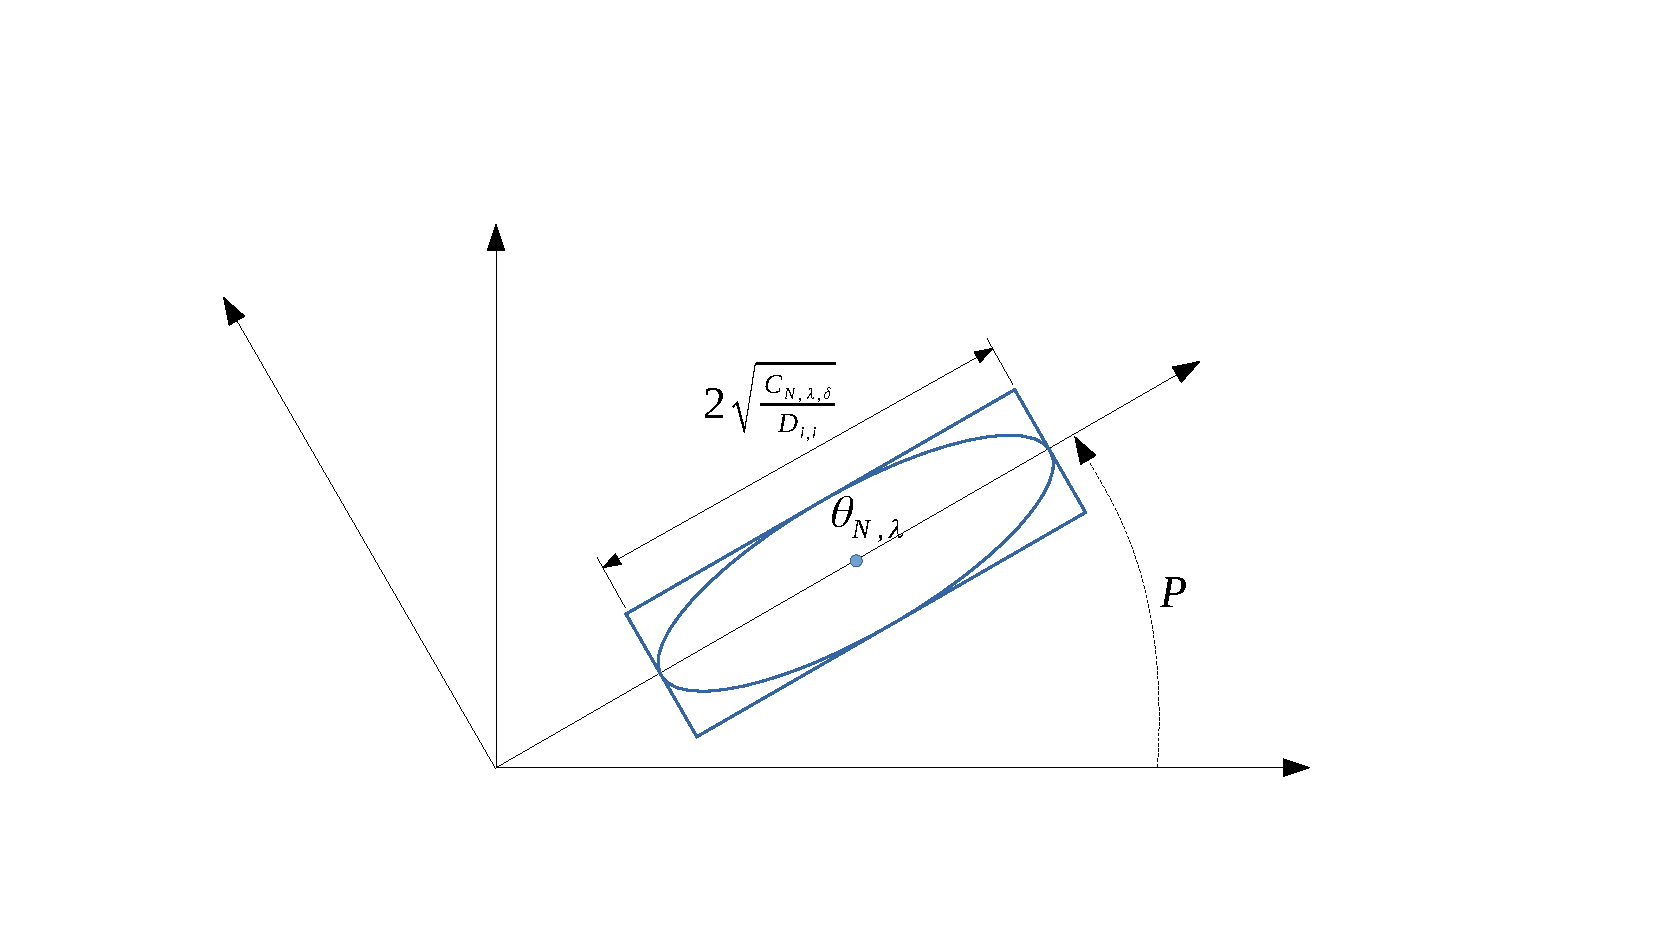
\includegraphics[trim={3.8cm, 2cm, 5cm, 3.8cm}, clip, width=0.7\linewidth]{img/ellipsoid_to_polytope}
		\caption{From the confidence ellipsoid $\cC_\confidence$ to its enclosing polytope $\cP_\confidence$}
		\label{fig:ellipsoid_to_polytope}
	\end{figure}
	
	\begin{lemma}[Confidence polytope]
		\label{lem:tight_polytope}
		\begin{leftbar}[lemmabar]
		We can enclose the confidence ellipsoid obtained in $\eqref{eq:confidence-ellipsoid}$ within a polytope
		\begin{equation}
		\cP = \left\{ A_{0}+\sum_{i=1}^{2^d}\lambda_{i}\Delta A_{i}: \lambda\in[0, 1]^{2^d},  \sum_{i=1}^{2^d}\lambda_{i}=1\right\}.
		\end{equation}
		with 
		\begin{align*}
		&h_k \text{ is the }k^\text{th}\text{ element of }\{-1,1\}^d\text{ for } k\in[2^d],\\
		&G_{N,\lambda} = PDP^{-1}, \quad \Delta\theta_k = \beta_{N}(\confidence)^{1/2} P^{-1}D^{-1/2} h_k, \\
		&A_0 = A + \theta_{N,\lambda}^\transp\phi, \quad \Delta A_k = \Delta\theta_k^\transp\phi.
		\end{align*}
		This conversion is illustrated in \Cref{fig:ellipsoid_to_polytope}.
		\end{leftbar}
	\end{lemma}

	\begin{proof}
		The ellipsoid in \eqref{eq:confidence-ellipsoid} is described by
		\begin{align*}
		\theta\in\confidenceset &\implies
		(\theta-\theta_{N,\lambda})^\transp G_{N,\lambda}(\theta-\theta_{N,\lambda}) \leq \beta_{N}(\confidence)\\
		&\implies (\theta'-\theta'_{N,\lambda})^\transp D (\theta'-\theta'_{N,\lambda}) \leq \beta_{N}(\confidence)\\
		&\implies \sum_{i=1}^d D_{i,i}(\theta'_i-\theta'_{N,\lambda,i})^2\leq \beta_{N}(\confidence)\\
		&\implies\forall i, |\theta'_i-\theta'_{N,\lambda,i}|\leq \beta_{N}(\confidence)^{1/2}D_{i,i}^{-1/2}
		\end{align*}
		This describes a $\Real^d$ box containing $\theta' = P\theta$, whose $k^\text{th}$ vertex is represented by $$\theta_{N,\lambda}' + \beta_{N}(\confidence)^{1/2}D^{-1/2} h_k.$$ We obtain the corresponding box on $\theta$ by transforming each vertex of the box with $P^{-1}$.
	\end{proof}

	
%		
%	\subsection{Experimental setting}
%	\label{sec:experimental-setting}
%	
%	In both experiments, we used $\discount=0.9$,  $\confidence=0.9$ and a planning budget $K=100$. The perturbations were sampled uniformly in $[-0.1, 0.1]^r$ while the measurements are Gaussian with covariance $\Sigma_r = 0.1 I_s$. 
%	
%	\subsection{Autonomous Driving}
%	
%	In the following, we describe the structure of the dynamical system $f$ representing the couplings and interactions between several vehicles.
%	
%	\paragraph{Kinematics}
%	
%	The kinematics of any vehicle $i\in[V]$ are represented by the Kinematic Bicycle Model:
%	\begin{align}
%	\dot{x}_i &= v_i\cos(\psi_i), \nonumber\\
%	\dot{y}_i &= v_i\sin(\psi_i), \nonumber\\
%	\dot{v}_i &= a_i, \nonumber\\
%	\dot{\psi}_i &= \frac{v_i}{l}tan(\beta_i), \nonumber
%	\end{align}
%	where $(x_i, y_i)$ is the vehicle position, $v_i$ is its forward velocity and $\psi_i$ is its heading, $l$ is the vehicle half-length, $a_i$ is the acceleration command and $\beta_i$ is the slip angle at the centre of gravity, used as a steering command.
%	
%	\paragraph{Longitudinal control}
%	Longitudinal behaviour is modelled by a linear controller using three features: a desired velocity, a braking term to drive slower than the front vehicle, and a braking term to respect a safe distance to the front vehicle.
%	
%	Denoting $f_i$ the index of the front vehicle preceding vehicle $i$, the acceleration command can be presented as follows:
%	\begin{equation*}
%	a_i = \begin{bmatrix}
%	\theta_{i,1} & \theta_{i,2} & \theta_{i,3}
%	\end{bmatrix} \begin{bmatrix}
%	v_0 - v_i \\
%	-(v_{f_i}-v_i)^- \\
%	-(x_{f_i} - x_i - (d_0 + v_iT))^- \\
%	\end{bmatrix},
%	\label{eq:theta_a}
%	\end{equation*}
%	where $v_0, d_0$ and $T$ respectively denote the speed limit, jam distance and time gap given by traffic rules.
%	
%	\paragraph{Lateral control}
%	
%	The lane $L_i$ with the lateral position $y_{L_i}$ and heading $\psi_{L_i}$ is tracked by a cascade controller of lateral position and heading $\beta_i$, which is selected in a way the closed-loop dynamics take the form
%	
%	\begin{align}
%	\label{eq:heading-command}
%	\dot{\psi}_i &= \theta_{i,5}\left(\psi_{L_i}+\sin^{-1}\left(\frac{\tilde{v}_{i,y}}{v_i}\right)-\psi_i\right),\\
%	\tilde{v}_{i,y} &= \theta_{i,4} (y_{L_i}-y_i). \nonumber
%	\end{align}
%	We assume that the drivers choose their steering command $\beta_i$ such that \eqref{eq:heading-command} is always achieved: $\beta_i = \tan^{-1}(\frac{l}{v_i}\dot{\psi}_i)$.
%	
%	\paragraph{LPV formulation}
%	
%	The system presented so far is non-linear and must be cast into the LPV form. We approximate the non-linearities induced by the trigonometric operators through equilibrium linearisation around $y_i=y_{L_i}$ and $\psi_i=\psi_{L_i}$.
%	
%	This yields the following longitudinal dynamics:
%	\begin{align*}
%	\dot{x}_i &= v_i,\\
%	\dot v_i &= \theta_{i,1} (v_0 - v_i) + \theta_{i,2} (v_{f_i} - v_i) + \theta_{i,3}(x_{f_i} - x_i - d_0 - v_i T),
%	\end{align*}
%	where $\theta_{i,2}$ and $\theta_{i,3}$ are set to $0$ whenever the corresponding features are not active.
%	
%	It can be rewritten in the form $$\dot{X} = \structureddynamics(X-X_c) + \omega.$$ For example, in the case of two vehicles only:
%	\begin{equation*}
%	X = \begin{bmatrix}
%	x_i \\
%	x_{f_i} \\
%	v_i \\
%	v_{f_i} \\
%	\end{bmatrix}
%	,\quad
%	X_c = \begin{bmatrix}
%	-d_0-v_0 T \\
%	0 \\
%	v_0\\
%	v_0 \\
%	\end{bmatrix}
%	,\quad
%	\omega = \begin{bmatrix}
%	v_0 \\
%	v_0 \\
%	0\\
%	0\\
%	\end{bmatrix}
%	\end{equation*}
%	
%	\begin{equation*}
%	\structureddynamics
%	=
%	\begin{blockarray}{ccccc}
%	& i & f_i & i & f_i \\
%	\begin{block}{c[cccc]}
%	i & 0 & 0 & 1 & 0 \\
%	f_i & 0 & 0 & 0 & 1 \\
%	i & -\theta_{i,3} & \theta_{i,3} & -\theta_{i,1}-\theta_{i,2}-\theta_{i,3} & \theta_{i,2} \\
%	f_i & 0 & 0 & 0 & -\theta_{f_i,1} \\
%	\end{block}
%	\end{blockarray}
%	\end{equation*}
%	
%	The lateral dynamics are in a similar form:
%	\begin{equation*}
%	\begin{bmatrix}
%	\dot{y}_i \\
%	\dot{\psi}_i \\
%	\end{bmatrix}
%	=
%	\begin{bmatrix}
%	0 & v_i \\
%	-\frac{\theta_{i,4} \theta_{i,5}}{v_i} & -\theta_{i,5}
%	\end{bmatrix}
%	\begin{bmatrix}
%	y_i - y_{L_i} \\
%	\psi_i - \psi_{L_i}
%	\end{bmatrix}
%	+
%	\begin{bmatrix}
%	v_i\psi_{L_i} \\
%	0
%	\end{bmatrix}
%	\end{equation*}
%	Here, the dependency in $v_i$ is seen as an uncertain parametric dependency, \ie $\theta_{i,6}=v_i$, with constant bounds assumed for $v_i$ using an overset of the longitudinal interval predictor.
%	
%	
%	\paragraph{Change of coordinates}
%	In both cases, the obtained polytope centre $A_0$ is non-Metzler.
%	We use the similarity transformation of coordinates of \citet{Efimov2013}. Precisely, we choose $\Theta$ such that for any $\theta\in\Theta$, $\structureddynamics$ is always diagonalisable with real eigenvalues, and perform an eigendecomposition to compute its change of basis matrix $Z$. The transformed system $X'=Z^{-1}(X-X_c)$ verifies \eqref{eq:confidence} with $A_0$ Metlzer as required to apply the interval predictor of \Cref{prop:predictor}. Finally, the obtained predictor is transformed back to the original coordinates $Z$ by using the following lemma:
%	\begin{lemma}[Interval arithmetic of \citealp{Efimov2012}]
%		\label{lem:interval} Let $x\in\mathbb{R}^{n}$ be a vector variable, $\underline{x}\le x\le\overline{x}$ for some $\underline{x},\overline{x}\in\mathbb{R}^{n}$. 
%		
%		\begin{enumerate}
%			\item If $A\in\Real^{m\times n}$ is a constant matrix, then
%			\begin{equation}
%			A^{+}\underline{x}-A^{-}\overline{x}\le Ax\le A^{+}\overline{x}-A^{-}\underline{x}.\label{eq:Interval1}
%			\end{equation}
%			\item If $A\in\Real^{m\times n}$ is a matrix variable and \textup{$\underline{A}\le A\le\overline{A}$} for some $\underline{A},\overline{A}\in\Real^{m\times n}$, then
%			\begin{gather}
%			\underline{A}^{+}\underline{x}^{+}-\overline{A}^{+}\underline{x}^{-}-\underline{A}^{-}\overline{x}^{+}+\overline{A}^{-}\overline{x}^{-}\leq Ax\label{eq:Interval2}\\
%			\leq\overline{A}^{+}\overline{x}^{+}-\underline{A}^{+}\overline{x}^{-}-\overline{A}^{-}\underline{x}^{+}+\underline{A}^{-}\underline{x}^{-}.\nonumber 
%			\end{gather}
%		\end{enumerate}
%	\end{lemma}
	
%	\paragraph{Actions}
%	
%	The action space $\cA$ is constituted of five actions: faster, slower, lane change to the right, lane change to the left, and no-op. They are implemented by a lateral linear controller that track a reference lateral position $y_L$, affected by the lane change actions, and a lateral longitudinal linear controller that tracks the desired velocity $v_0$, affected by the faster and slower actions.
%	
%	\paragraph{Reward}
%	
%	The reward function $R$ is the following:
%	\[
%	R(x) = 
%	\begin{cases}
%	1 & \text{if the ego-vehicle is at full velocity;}\\
%	0 & \text{if the ego-vehicle has collided with another vehicle;}\\
%	0.5 & \text{else.}
%	\end{cases}\]
	

%\end{subappendices}


\chapter*{Part Conclusion\\ {\LARGE Review of our Requirements}}
\mtcaddchapter[Part Conclusion]

Again, in \Cref{tab:part-3-conclusion} we discuss whether the methods developed in \Cref{part:3} address the challenges identified in \Cref{chapter:1}.

\begin{table}[H]
	\begin{tabularx}{\linewidth}{p{2.2cm}cX}
		\toprule
		Criterion & & Description \\
		\midrule
		\textbf{\makecell[l]{Social \\Awareness}} & {\Large $\hlgb{\checkmark}$} & In \Cref{chapter:6,chapter:7}, the planning algorithm relies on a predictive model $\dot{x_i} = f_i(x, u)$ in which the motion of a vehicle $i\in[N_v]$ is coupled to that of other vehicles $x = [x_0, x_1, \dots x_{N_v}]$ in the scene, to account for driving interactions. \\
		\textbf{\makecell[l]{Sample \\ Efficiency}} & {\Large $\hlgb{\checkmark}$} & For \emph{model estimation}, we rely in \Cref{chapter:7} on a structured parametrised model $\dot x = A(\theta)x + Bu$ which incorporates priors over car-like kinematics (non-holonomic) and human driving behaviours (lane following, cruise control). The \emph{planning} step can benefit from the contributions of \Cref{chapter:6} on optimistic tree-based planning, such as merging the states of overlapping sampled trajectories. \\
		\textbf{Safety} & {\Large $\hlgb{\checkmark}$} & Two other notions of risk were introduced in \Cref{chapter:7}: first as a hard constraint $x\in\safestates,\,u\in\safecontrols$ under bounded disturbances and parametric model uncertainty; and second, as a minimax objective that produces risk-averse behaviours by evaluating the worst possible outcome under said disturbances and model uncertainty. \\
		\textbf{Balance between safety and efficiency} & {\Large $\hlgb{\checkmark}$} & The conservativeness of the robust \gls{MPC} algorithms of \Cref{chapter:7} can be tuned by adjusting the confidence level $\confidence$ to trade-off the error probability with the size of the confidence region $\cC_{[N],\delta}$; or by considering additional modelling assumptions $(A, \phi)$ in the multi-model perspective, which will increase robustness at the expense of efficiency.\\
		\bottomrule
	\end{tabularx}
	\caption{Do the methods of \Cref{part:3} comply with the specifications of \Cref{chapter:1}?}
	\label{tab:part-3-conclusion}
\end{table}
